% Suggested LaTeX style template for Masters project report submitted at the
% Department of Computer Science and Technology
%
% Markus Kuhn, May 2022
% (borrowing elements from an earlier template by Steven Hand)

\documentclass[12pt,a4paper]{report}

\usepackage[top=20mm, bottom=20mm, left=25mm, right=25mm]{geometry}
% append option ",openright" after "twoside" if you prefer each chapter
% to start on a recto (odd-numbered) page in a double-sided printout

\usepackage[pdfborder={0 0 0}]{hyperref}  % turns references into hyperlinks
\usepackage[vmargin=20mm,hmargin=25mm]{geometry}  % adjust page margins
\usepackage{graphicx} % allows inclusion of PDF, PNG and JPG images
\usepackage{parskip}  % separate paragraphs with vertical space
                      % instead of indenting their first line
\usepackage{setspace} % for \onehalfspacing
\usepackage{refcount} % for counting pages
\usepackage{upquote}  % for correct quotation marks in verbatim text
\usepackage[numbers,compress,sort]{natbib}

\usepackage{algorithm}
\usepackage{algpseudocode}
\usepackage{booktabs}            % professional-quality tables
\usepackage{multirow}            % tabular cells spanning multiple rows
\usepackage{amsfonts}            % blackboard math symbols
\usepackage{graphicx}            % figures
\usepackage{duckuments}          % sample images
\usepackage{amssymb}
\usepackage{physics}
\usepackage{amsmath}
\usepackage{tikz}
\usepackage{mathdots}
\usepackage{yhmath}
\usepackage{cancel}
\usepackage{color}
\usepackage{siunitx}
\usepackage{array}
\usepackage{multirow}
\usepackage{amssymb}
\usepackage{gensymb}
\usepackage{tabularx}
\usepackage{extarrows}
\usepackage{booktabs}
\usetikzlibrary{fadings}
\usetikzlibrary{patterns}
\usetikzlibrary{shadows.blur}
\usetikzlibrary{shapes}
\usepackage{booktabs}
\usepackage{bbm}
\usepackage{subfigure}


\newif\ifsubmission % Boolean flag for distinguishing submitted/final version

% Change the following lines to your own project title, name, college, course
\title{Structure-informed protein engineering using equivariant graph neural networks}
\author{Antonia-Irina Boca}
\date{May 2023}
\newcommand{\candidatenumber}{2485A}
\newcommand{\college}{King's College}
\newcommand{\course}{Computer Science Tripos, Part III}
%\newcommand{\course}{Master of Philosophy in Advanced Computer Science}

% Select which version this is:
% For the (anonymous) submission (without your name or acknowledgements)
% uncomment the following line (or let the makefile do this for you)
\submissiontrue
% For the final version (with your name) leave the above commented.

 \clubpenalty = 10000
 \widowpenalty = 10000
 \displaywidowpenalty = 10000
 
\begin{document}
%TC:ignore

% \printlength\textwidth
\begin{sffamily} % use a sans-serif font for the pro-forma cover sheet

\begin{titlepage}
\makeatletter

% University logo with shield hanging in left margin
\hspace*{-14mm}
\includegraphics[width=65mm]{logo-dcst-colour}

\ifsubmission

% submission proforma cover page for blind marking
\begin{Large}
\vspace{20mm}
Research project report title page

\vspace{35mm}
Candidate \candidatenumber

\vspace{42mm}
\textsl{``\@title''}

\end{Large}

\else

% regular cover page
\begin{center}
\Huge
\vspace{\fill}

\@title
\vspace{\fill}

\@author
\vspace{10mm}

\Large
\college
\vspace{\fill}

\@date
\vspace{\fill}

\end{center}

\fi

\vspace{\fill}
\begin{center}
Submitted in partial fulfillment of the requirements for the\\
\course
\end{center}

\makeatother
\end{titlepage}

\newpage

Total page count: \pageref{lastpage}

% calculate number of pages from
% \label{firstcontentpage} to \label{lastcontentpage} inclusive
\makeatletter
\@tempcnta=\getpagerefnumber{lastcontentpage}\relax%
\advance\@tempcnta by -\getpagerefnumber{firstcontentpage}%
\advance\@tempcnta by 1%
\xdef\contentpages{\the\@tempcnta}%
\makeatother

Main chapters (excluding front-matter, references and appendix):
\contentpages~pages
(pp~\pageref{firstcontentpage}--\pageref{lastcontentpage})

Main chapters word count: 11664

Methodology used to generate that word count:

\begin{quote}
\begin{verbatim}
$ ./texcount.pl -inc -total -sum masters-report/report.tex

Total
Sum count: 11673
Words in text: 10450
Words in headers: 231
Words outside text (captions, etc.): 753
Number of headers: 87
Number of floats/tables/figures: 25
Number of math inlines: 201
Number of math displayed: 38
Files: 8
\end{verbatim}
\end{quote}

\end{sffamily}

\vspace{\fill}
\onehalfspacing
\ifsubmission\else\makeatletter
\textbf{\Huge Declaration}
\vspace{40pt}

I, \@author\ of \college, being a candidate for the \course, hereby
declare that this report and the work described in it are my own work,
unaided except as may be specified below, and that the report does not
contain material that has already been used to any substantial extent
for a comparable purpose.

% Add here things like: Figure X is the work of Y, etc.

\bigskip 
\textbf{Signed:} Antonia-Irina Boca

\bigskip
\textbf{Date:} \today
\vspace{\fill}
\makeatother\fi

\chapter*{Abstract}

Computational protein engineering plays a crucial role in advancing scientific research and technological applications in various fields, with pre-trained machine learning models being successful in many protein engineering tasks. 
Most notably, models trained on protein sequences have achieved state-of-the-art performance on protein fitness prediction while models trained on protein structures have been used experimentally to develop proteins with enhanced functions. 

Despite the experimental success of pre-trained structural methods for protein engineering \cite{torng20173d, Lu2022}, several crucial aspects remain unexplored. Firstly, these methods have not been systematically compared with sequence-based approaches using the same datasets. Secondly, their potential to augment assay labelled data, when available, has not been evaluated.

This project initially aimed to evaluate the performance of equivariant graph neural networks (EGNNs) in predicting amino acid residue identity based on local atomic environments, and I report a \textbf{new state-of-the-art} performance on this task. 

I extended the project's scope to utilise these trained models as structure-based models for proposing single-point mutations in proteins. By leveraging the inferred biophysical knowledge derived from pre-training on local atomic environments, these EGNN models can act as unsupervised predictors for the fitness of mutated proteins. I explore systematic approaches to extract candidate mutations based on the models' confidence when dealing with targeted positions. 

I find that structural models based on EGNNs have a competitive performance to sequence-based approaches, while being trained on \textbf{15,909x} fewer of molecules. Additionally, I show how the positional scores generated by these models can be used to augment linear models for protein fitness prediction, effectively operating in a low-data regime: ridge regression models augmented with scores from EGNNs can surpass the performance of pre-trained sequence models with as few as 100 data points.

This project has made significant strides in understanding EGNNs' potential to improve protein design and optimisation, with results indicating the efficacy and potential of structure-based models in addressing key challenges in protein engineering.

\ifsubmission\else
% not included in submission for blind marking:

\chapter*{Acknowledgements}

This project would not have been possible without the wonderful
support of Simon Mathis, whose invaluable guidance and expertise in the field of biology have been instrumental in shaping this dissertation. As a computer scientist with limited knowledge of biology, I was fortunate to have Simon as a mentor that patiently taught me the fundamental concepts and provided me with the necessary tools to navigate this interdisciplinary research project. 

\fi
\cleardoublepage % preserve page numbers after missing acknowledgements

\tableofcontents
\listoffigures
\listoftables
%TC:endignore
\chapter{Introduction}

\label{firstcontentpage} % start page count here
Proteins are complex macromolecules that lie the foundation for all living life on Earth. From providing structural support to cells and tissues through proteins like collagen and keratin, to acting as catalysts for chemical reactions such as the digestion of starch, proteins maintain the normal functioning of living organisms. Since they are fundamental to so many biological processes that make life possible, it is no wonder that the malfunction of proteins can have devastating effects on the health of individuals. To take one example, Parkinson's disease, a chronic degenerative disease that affects the motor system in humans, arises as a result of the aggregation of alpha-sinuclein protein in the brain, a molecule that regulates synaptic vesicle trafficking and subsequent neurotransmitter release.

\section{Computational protein engineering}
Protein engineering is a field of biotechnology that aims to artificially modify existing proteins in order to enhance their properties or create new functions. The field also looks at ways to cure diseases that are the result of malfunctioning biological processes and proteins. For example, as early as 1988, \citet{insulin} induced mutations into the insulin agents used to treat diabetes in order to make them easier to be absorbed by the body and better mimic the action of the naturally-produced insulin hormone. 

Albeit it is a promising field, protein engineering can be a costly, labour intensive process in which researchers have to first determine the mutations most likely to be successful for the task at hand and then experimentally validate them. Moreover, when the discovery process is done experimentally, it may not even be possible, in some cases, to determine the structure of certain unstable proteins. \textit{Computational protein engineering} aims to optimise this exploratory process by using computational methods to accelerate the generation of the most likely to be successful mutations. For example, the last few years have seen a major breakthrough in \textit{protein folding prediction} through the AlphaFold program developed by DeepMind \cite{alphafold}, that uses machine learning (ML) techniques to learn to predict protein structures from their associated sequences. Before AlphaFold, all protein structures would be discovered experimentally in the wet lab over the course of many hours of intensive and expensive labour. With this new computational method, however, researchers can now receive the highly accurate structure prediction of a protein sequence within seconds, thereby making the whole discovery part of the drug design process much faster and efficient. Therefore, computational methods can overcome the limitations of traditional ones by exploring protein structures that have not been experimentally observed yet. 

\section{Equivariant graph neural networks}
This project proposes a novel approach to mutation generation for proteins through the usage of graph neural networks (GNNs). Neural networks are computing systems with interconnected nodes that perform operations on the input data in order to solve a specific task. The nodes' coefficients (commonly called weights) are adjusted by \textit{learning} to approximate functions of the inputs using massive amounts of training examples. Neural networks have become the most widespread approach to machine learning, and are heavily integrated in the fabric of modern society - from content recommendation systems used on social media platforms to language translation and trading on the stock market, almost any digital app can nowadays be augmented with one of the available flavours of neural networks. 

Graph neural networks have gained popularity in the last couple of years and have become the most promising machine learning technique for processing graph information. All GNNs use some form of \textit{neural message passing}, where messages are exchanged between nodes and updated using a neural network \citep{gilmer2017neural}. Many GNNs operate on graphs that represent abstract collections of objects, such as social networks; many, if not all, of the original GNN structures that were proposed would only be able to process scalar features (e.g., in a social network these would be age, gender, social background, etc). However, many real-world graphs are inherently geometric, with nodes having positions in 3D space. To deal with these graphs, the message-passing paradigm was extended to include \textbf{Equivariant Graph Neural Networks} (EGNNs), a type of GNNs that can process information in such a way that preserves the structural properties of the nodes' features. The equivariance and invariance of neural networks, is not, however, a new concept: convolutional neural networks, regarded as the de-facto ML architecture to process image data, already respect the concept of translation equivariance and invariance, as illustrated in Figure \ref{cnn-invariance}. As one can see, a cat stays a cat no matter where it is translated within the picture. 
\begin{figure}
    \centering
    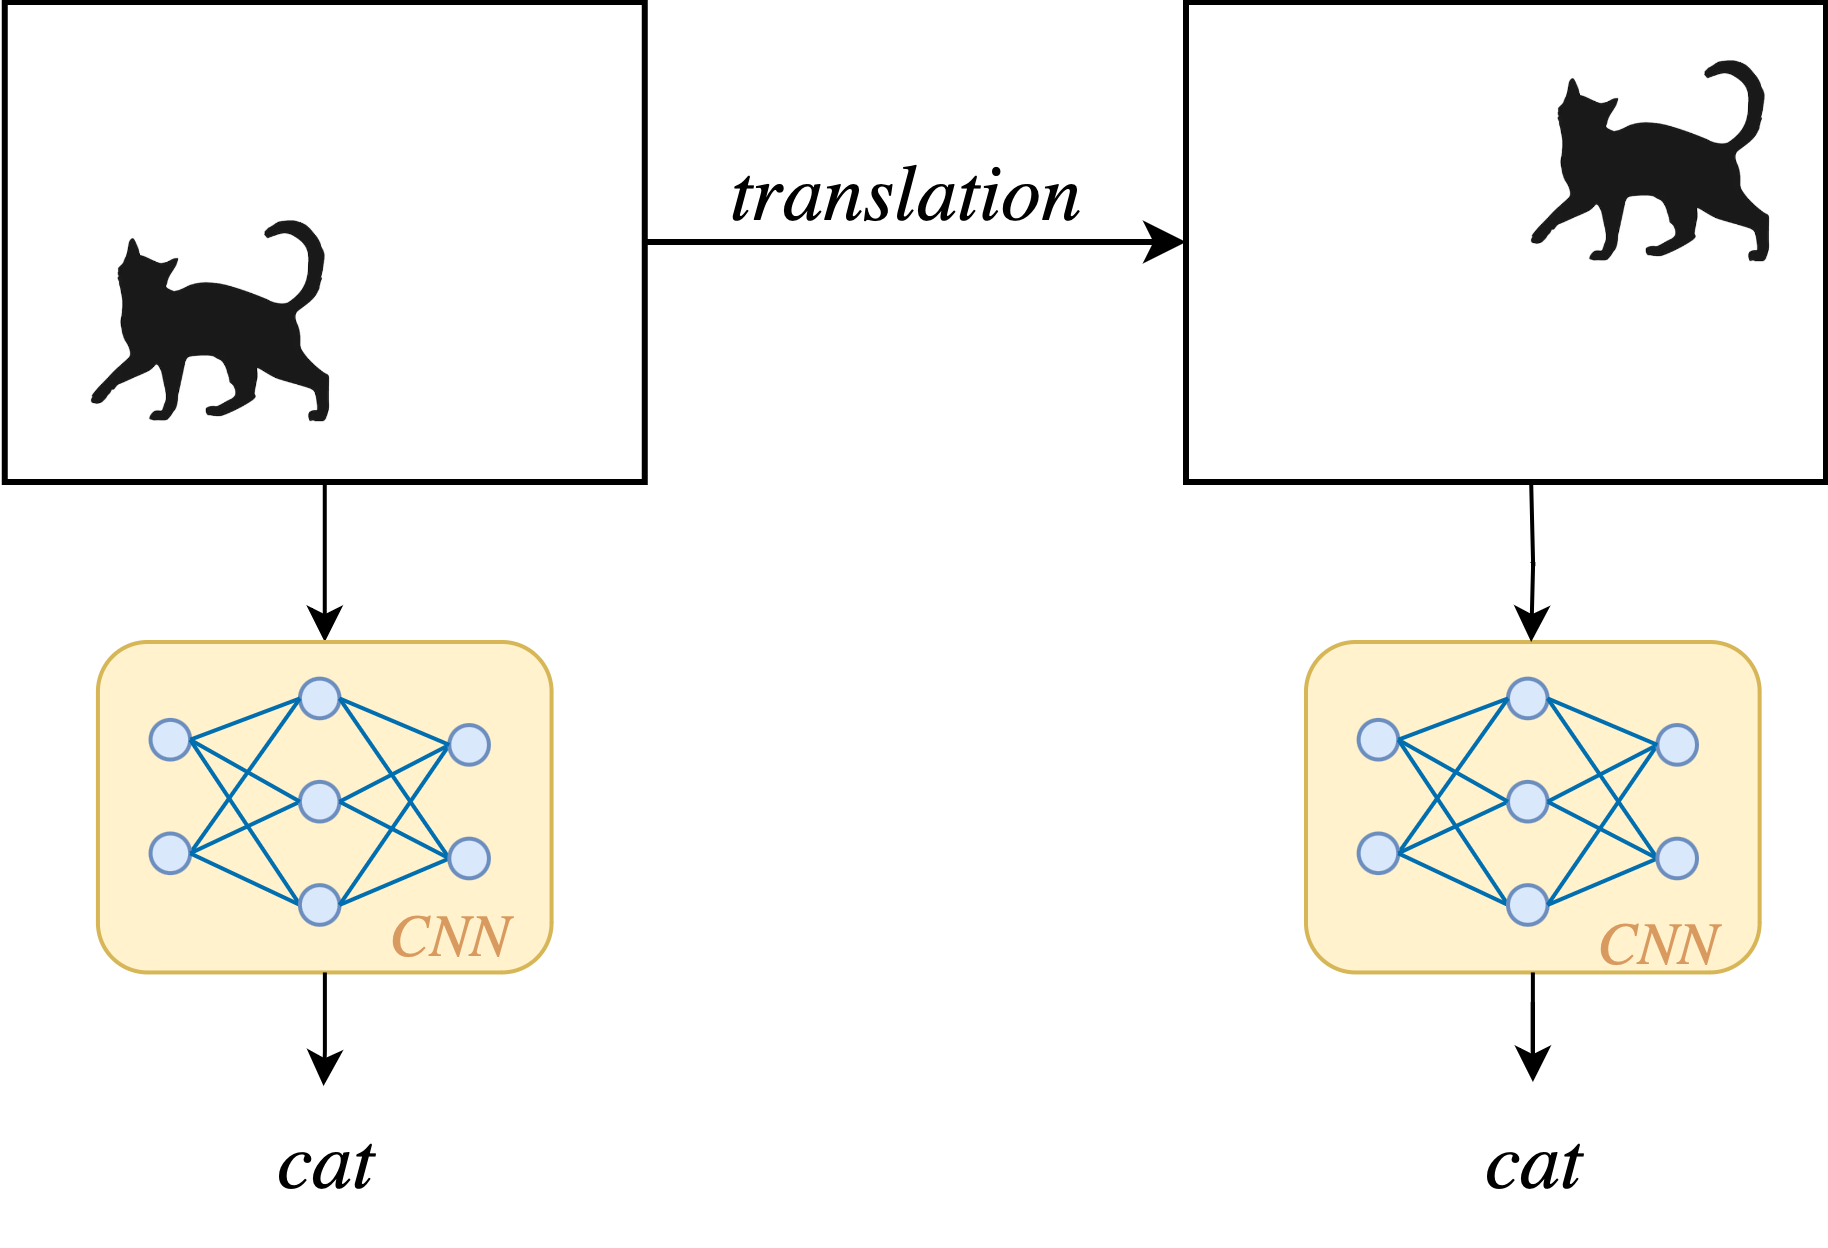
\includegraphics[scale=0.6]{masters-report/figures/cnn-invariance.png}
    \caption{Translation invariance in a CNN.}
    \label{cnn-invariance}
\end{figure}

Protein structures can be represented as graphs with nodes corresponding to atoms. Each atom's scalar feature is its atom type (e.g., Carbon, Nitrogen, Hidrogen, etc.) and its vector feature is the atom's position in 3D space. Using this representation, we can design and train GNNs that are  \textit{equivariant to 3D rotations and translations} to perform a range of molecular tasks. This has approach has already been proven successful on the scoring of protein-ligand complexes \cite{egnn-application-1} or model quality assessment (MQA) \cite{gvp1}.

\section{Unsupervised EGNNs for mutation generation}

The original aim of this project was to evaluate the performance of a handful of newly proposed EGNNs architectures to the molecular task of amino-acid residue identity prediction, also known as the RES task \cite{atom-3d}. This task involves training an ML model to predict the missing amino-acid in a protein given the surrounding atomic environment. 

\textbf{We extend} the original scope of the project to use these trained EGNN models to propose single-point mutations given a protein structure, thereby putting to use the biophysical knowledge that these models have inferred from training on the RES task. These models effectively act as \textbf{unsupervised} models for predicting the \textit{fitness} of a mutated protein, i.e., its ability to perform its biological function more effectively than the wildtype (the non-mutated protein). The idea behind our approach is to use the trained EGNN models to score the existence of a certain amino-acid at a target position in a protein sequence. Figure \ref{idea} illustrates this concept visually. 

\begin{figure}[!h]
    \centering
    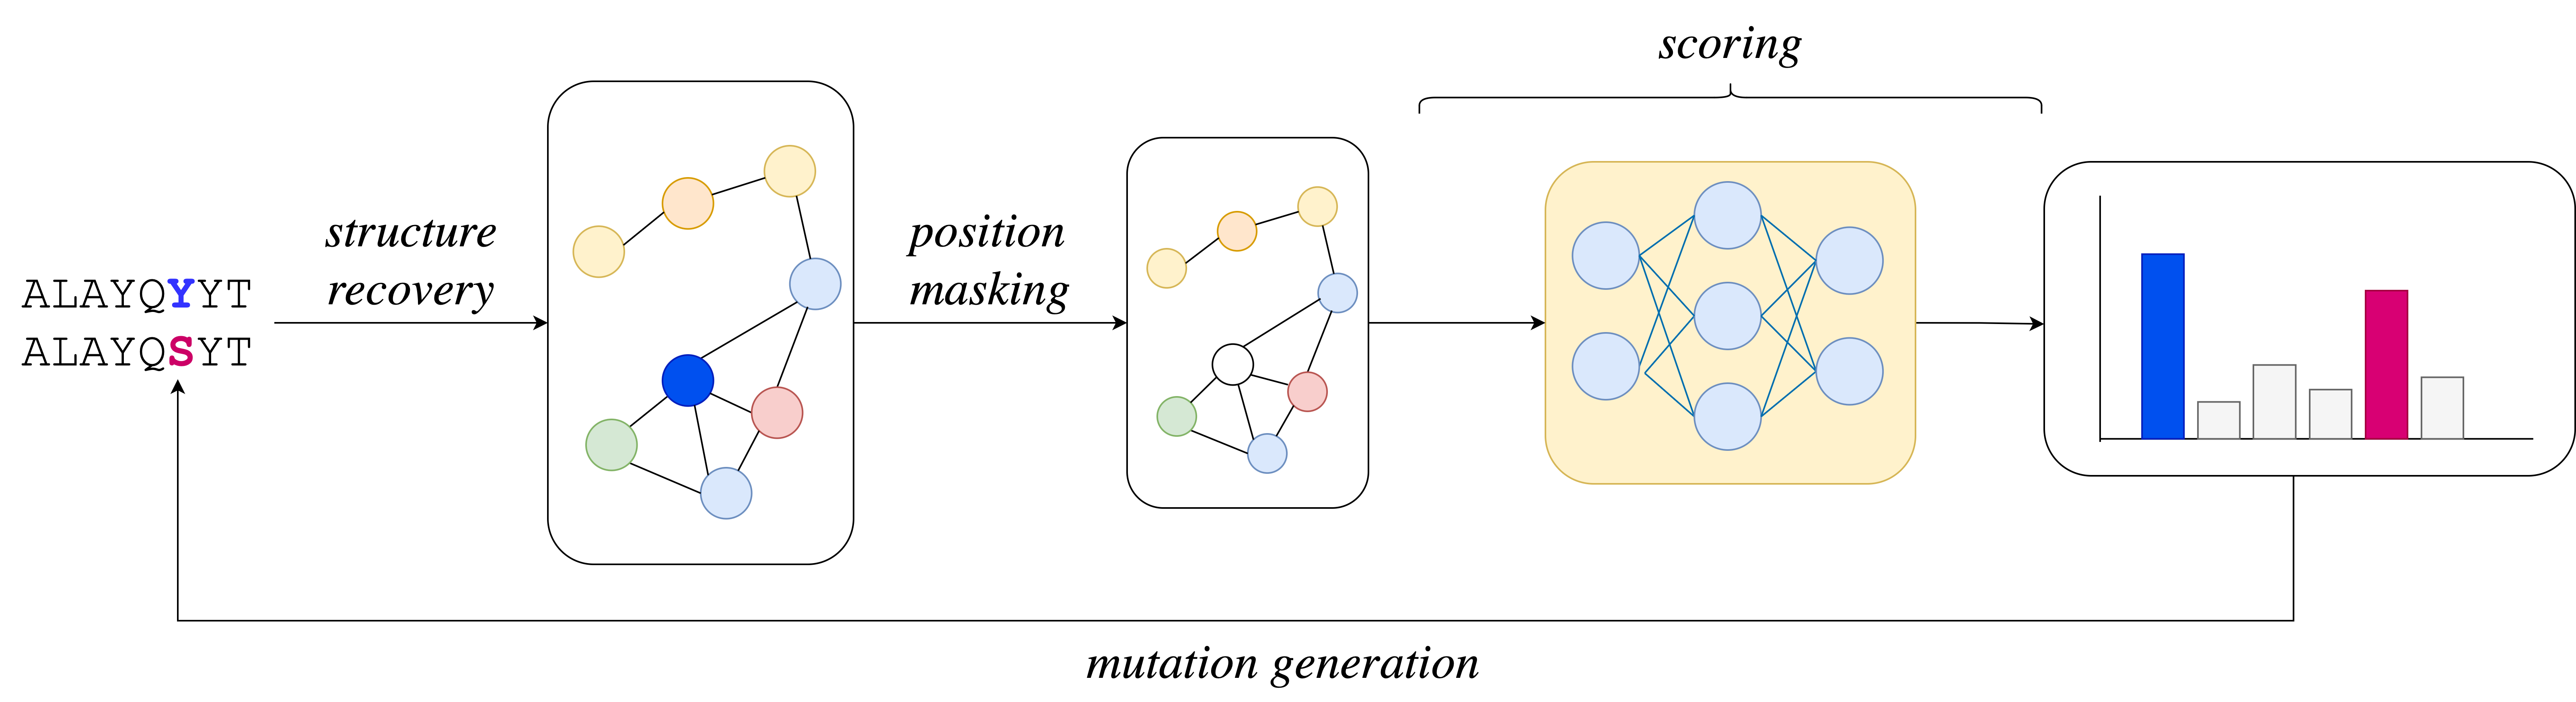
\includegraphics[width=\textwidth]{masters-report/figures/mutation_generation_2.png}
    \caption{The idea behind our mutation generation strategy.}
    \label{idea}
\end{figure}

By targeting each position of an amino-acid sequence in turn, we observe the positions at which the EGNN model is \textit{least confident}. This could be an indication that the position is a good candidate for mutations. Moreover, by looking the scores of all amino-acids at a certain position we can understand what the model thinks are the best matches for that position. The project will compare a couple of systematic approaches for extracting the candidate mutations by looking at both the models' confidence when dealing with amino-acids at targeted positions. 

\section{Augmented linear models for protein fitness prediction}

Having powerful, yet unsupervised models aids the exploratory process when dealing with new proteins – this project acts as a proof-of-concept to how EGNNs can become tools that help researchers accelerate the study of new proteins. Conversely, when data about a mutated sequence's fitness is already available to some extent, we can combine it with the EGNN models proposed in this project in order to create models that effectively operate in a \textbf{low-data regime} and take full advantage of both the latent knowledge of the unsupervised model and the task-specific information provided by the already existing, albeit limited, data. 

To this extent, we propose an \textbf{augmented} ridge regression model that learns to predict the protein fitness of single-point mutated sequences by combining the information about the amino-acid present at each position with the EGNN score for the specified mutation. Although the usage of regression models for fitness prediction was first studied by \citet{chloe-hsu}, we are the first to evaluate this approach using EGNNs and find that it outperforms state-of-the-art transformer models when predicting the fitness of better-than-wildtype sequences. 

\section{Contributions}

\chapter{Background}

{
    \color{red}
    \begin{enumerate}
        \item Biological background
        \begin{enumerate}
            \item residue identity prediction
            \item atomic environments 
            \item SMILES representation?
        \end{enumerate}
        \item Machine learning background
        \begin{enumerate}
            \item neural networks
            \item graph neural networks
            \item equivariant graph neural networks
            \item representing residues as graphs
        \end{enumerate}
    \end{enumerate}
}

\section{Biological background}
\subsection{Proteins}
\begin{figure}
    \centering
    \begin{tikzpicture}
    \node (acidone) {\chemfig{N(-[3]H)(-[5]H)-C(-[2]H)(-[6]R_1)-C(-[1]{\color{blue}OH})(=[7]O)}};
    \node[right of=acidone, xshift=5cm] (acidtwo) {\chemfig{N(-[3]H)(-[5]{\color{blue}H})-C(-[2]H)(-[6]R_2)-C(-[1]OH)(=[7]O)}};
    \draw[->,thick] ($(acidone.east)!0.5!(acidtwo.west)$) ++(0, -1.7cm) -- ++(0,-1cm) node[right] {};
    \node[below of=acidone, xshift=3cm, yshift=-4.2cm] (residue) 
        {\chemfig{N(-[3]H)(-[5]H)-C(-[2]H)(-[6]R_1)-C(=[7]O)-[1,,,,blue]N(-[3]H)-C(-[2]H)(-[6]R_2)-C(=[7]O)(-[1]OH)}};
    
    \node[below of=residue, yshift=-1.3cm, xshift=-1.8cm] (res1) {\textit{residue 1}};
    \node[below of=residue, yshift=-1.3cm, xshift=1.8cm] (res1) {\textit{residue 2}};
    \end{tikzpicture}
\end{figure}
\subsection{Residue identity prediction}

\section{Machine learning background}
\subsection{Graph Neural Networks}
\subsection{Equivariant Graph Neural Networks}
\subsection{Representing residues as graphs}


\chapter{Related work}

The field of protein engineering has witnessed many advancements in recent years, fueled by the growing demand for designing novel proteins with enhanced functionalities. In this context, machine learning techniques have emerged as powerful tools for analysing and manipulating proteins. 

Many state-of-the-art approaches that use machine learning focus on the sequence of a protein, rather than its structure, because protein sequences are more widely available. In this chapter, we explore the existing body of literature surrounding the most powerful techniques to assess the fitness of mutations, as well as discussing the emerging techniques that aim to take advantage of the structure of proteins by highlighting the key contributions, methodologies, and findings that have paved the way for this research area.

\section{Sequence-based protein engineering}

\subsection{Multiple sequence alignments}
Many approaches to protein engineering use multiple sequence alignments (MSAs) to study and propose mutations for each protein sequence. In bioinformatics, sequence alignment refers to arranging sequences of proteins to identify regions of similarity that may indicate evolutionary relationships, which provide insight into the function of the aligned proteins. By training machine learning models on MSAs, a coordinate system of the aligned sequences is developed, allowing the model to score amino acids at a given position and to compare them to the rest of the training set. This was the approach taken first by \citet{deepsequence}, who propose a Variational Autoencoder, DeepSequence, trained on protein-specific MSAs to understand the most likely amino acids to be present at certain positions in the sequence. This approach was later expanded by \citet{EVE}, who proposed EVE, a model that predicts the fitness of human variants in disease-related genes. 

\subsection{Large language models}
% The usage of MSAs, however, has some limitations. Most importantly, they cannot deal with non-alignable proteins; these are proteins have diverged significantly over evolutionary time and share very little sequence similarity with other proteins. In such cases, traditional sequence alignment methods may not be able to identify regions of similarity that help the models assess the quality of mutations. Due to this limitation, some researchers have started pursuing an alternative line of inquiry, in which models do not need MSAs.  This line of inquiry has taken advantage of the advances made in the Natural Language Processing field to understand sequences, with \citet{alley2019unified} and \citet{heinzinger2019modeling} each training Long Short-Term Memory Networks \cite{lstms} across many protein families.

% The rise of the Transformer architecture, first introduced by \citet{vaswani2017attention}, has resulted in significant performance improvements on sequence-based tasks. \citet{madani2020progen, nambiar2020transforming, rives2021biological} were the first to propose the usage of transformers to model protein sequences. In a line of research that combines both the usage of MSAs and the usage of large language models, \citet{Rao2020} introduced the MSA Transfomer, a model trained on a large collection of MSA families. In opposition, \citet{elnaggar2021prottrans} and \citet{meier2021language} developed transformers trained exclusively on non-aligned proteins from protein databases. In parallel, \citet{vig2020bertology} showed how the self-attention mechanism that is characteristic of the Transformer architecture actually captures the underlying structure of protein sequences and can build complex biophysical properties as the number of self-attention layers increases. 

While MSAs provide good evolutionary insights, they need to be re-trained for each protein of interest, and have difficulties dealing with non-alignable proteins that have diverged significantly over time. To address this, researchers have explored an alternative approach that leverages Natural Language Processing techniques. \citet{alley2019unified} and \citet{heinzinger2019modeling} trained Long Short-Term Memory Networks (LSTMs) to understand protein sequences across various families.

The Transformer architecture, introduced by \citet{vaswani2017attention}, has shown significant performance improvements for sequence-based tasks. \citet{madani2020progen, nambiar2020transforming, rives2021biological} proposed the use of transformers for modeling protein sequences. \citet{Rao2020} introduced the MSA Transformer, which combines MSAs and large language models. Conversely, \citet{elnaggar2021prottrans} and \citet{meier2021language} developed transformers exclusively trained on non-aligned proteins. Additionally, \citet{vig2020bertology} demonstrated how the self-attention mechanism in Transformers captures features that correlate with the structure of protein sequences and can model complex biophysical properties with increased self-attention layers.

Most recently, \citet{tranception} have proposed an auto-regressive transformer model, Tranception, that achieves state-of-the-art results on their newly compiled benchmark dataset, ProteinGym, that spans 87 DMS assays,\footnote{Deep mutational scanning is a high-throughput functional assay that measures the effect of every genetic change at every site in a protein.} containing the protein fitness of over 1.5M variants. However, as it will be shown in this project, while its performance ranks highest for predicting fitness across all variants, the method does not perform well on predicting fitness of variants that are \textit{better than the wildtype sequence}. In part, this can be explained by the fact that the vast majority of protein variants will perform worse than the wildtype protein, so even very powerful models trained on predicting protein fitness are more likely to see bad variants than good ones. 

Tranception is trained on UniRef100 \cite{uniref}, a database containing sequences in UniProt, a freely accessible knowledgebase of protein sequence and functional information. UniRef100 contains over 350 million sequences. In contrast, the structural approach taken in this project only uses local environments sampled from 22K molecules, thereby training models with similar performance on suggesting better than the wildtype mutations by using \textbf{15,909x} fewer data points. 

\section{Structure-based protein engineering}
Protein sequences are more readily available in large quantities than their associated structures. Up until 2 years ago, when \citet{alphafold} released the breakthrough AlphaFold2 machine learning model that can predict the structure of a protein given its sequence, it was estimated that we only have available structures for 17\% for all proteins found in humans, by some metrics \cite{portapardo2022structural} – highly confident predictions made by AlphaFold2 have increased this coverage to 50\%.   

Structure-informed protein engineering using deep learning techniques is, therefore, a young research field, with many more challenges other than the lack of available structures to train models on: even when structure datasets, like ATOM3D \cite{atom-3d}, are made available, the complex symmetries exhibited by proteins require specialised models that can process 3D Euclidean coordinates. A first strategy was proposed by \citet{torng20173d}, who use 3D-CNNs to process the structure of the protein. 
The approach they take is to discretise the protein into cubic grids of a fixed size and extracting the ``average'' atom features present in every cube, as shown in Figure \ref{3d-cnn}. The features are then processed in a similar manner to how image data is processed by 2D-CNNs. 
\begin{figure}[!htb]
    \centering
    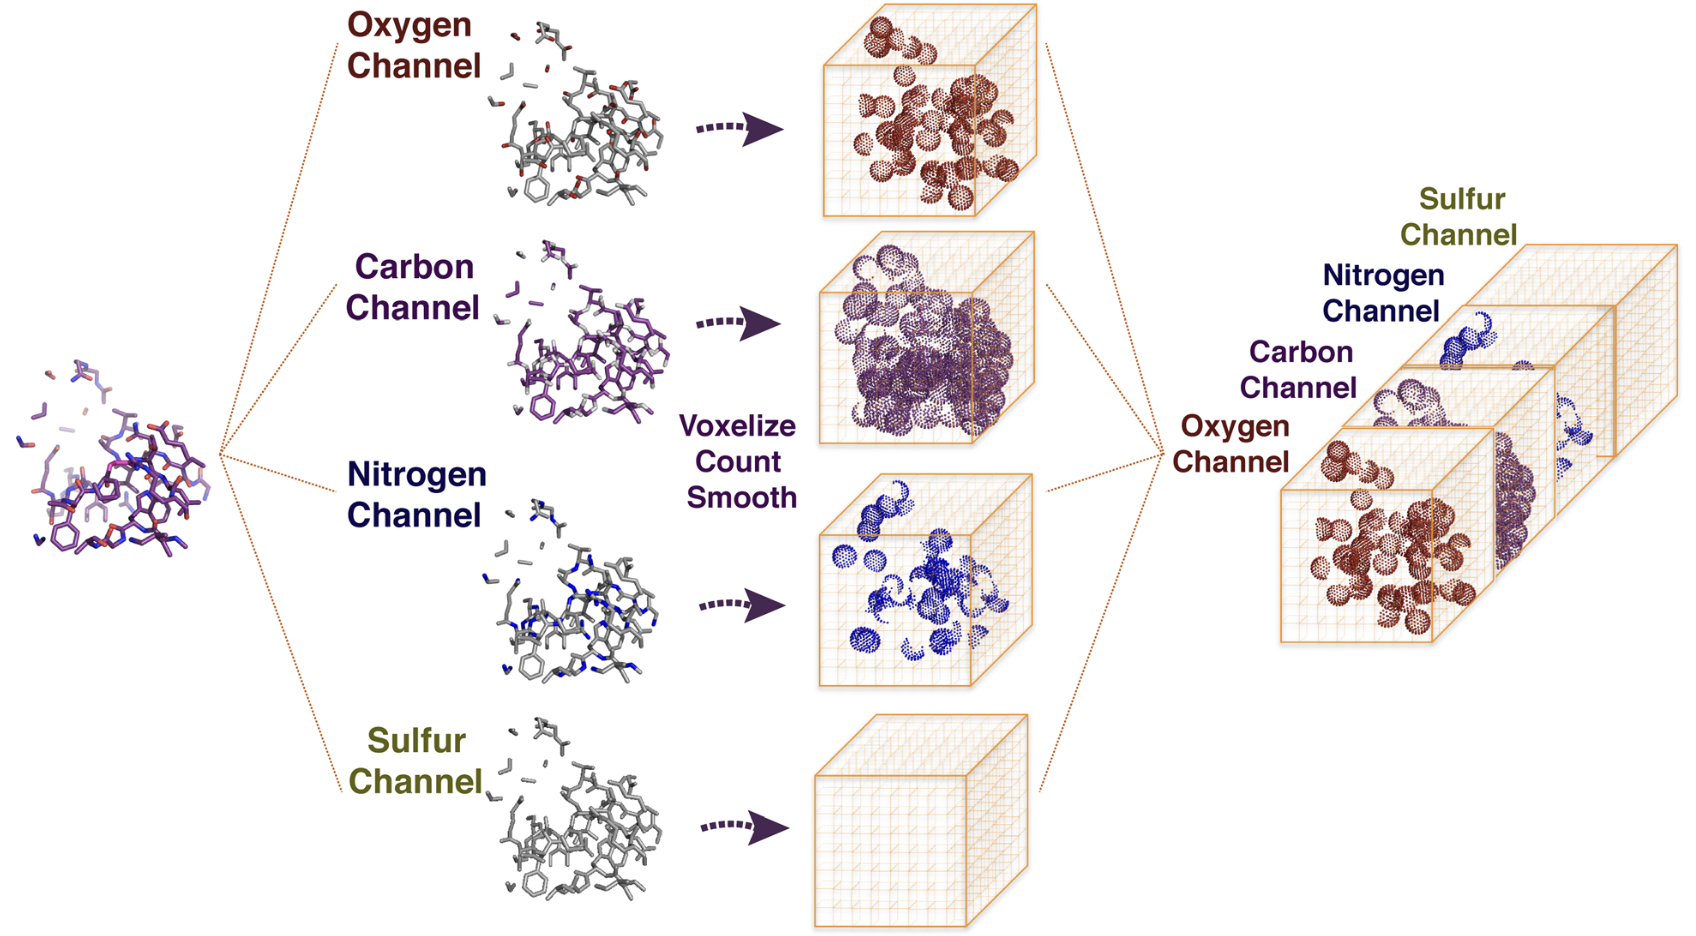
\includegraphics[width=0.7\textwidth]{masters-report/figures/3d-cnn.png}
    \caption{Local environment processing with 3D-CNNs. The local structure is first decomposed into separate atom channels. Each atom type channel is divided into 3D voxels, with each voxel recording the presence of that atom type within its boundaries. The decomposed approximation of the initial structure is then processed as it is usual with CNNs. Image taken from \cite{torng20173d}.}
    \label{3d-cnn}
\end{figure}

Based on this approach, \citet{mutcompute} introduce MutCompute, a model trained to predict the identity of an amino acid based on its local environment. \citet{mutcompute} use a different, proprietary dataset to the one used in this project. In a similar manner to the one we employ, the scores generated by the trained model are used for mutation generation across 3 proteins. More recently, \citet{Lu2022} also use MutCompute to engineer more thermally stable plastic degrading enzymes. 

In contrast to \citet{mutcompute} and \citet{Lu2022}, in this project we avoid the need of discretising the protein structure into cubic grids and therefore take full advantage of the structural properties of the atomic envrionment. To this extent, we employ equivariant graph neural networks (EGNNs), a type of GNNs that use specialised operations and architectures that preserve the structural properties of certain symmetry groups – in our case, the SE(3) group. 

\section{Equivariant graph neural networks}

Graph neural networks were proposed as a solution to dealing with graph-based data through the message-passing framework. One of the first successful architectures was the GCN, proposed by \citet{gcn}. 
Traditional GNNs operate on graphs that represent abstract collections of objects, such as social networks. To deal with geometric graphs, the message-passing paradigm was extended to include \textbf{equivariant graph neural networks} (EGNNs), a type of GNNs that can transform \textit{vector features} under some group action.

One line of research into EGNNs achieves equivariance in the E(3) and SE(3) spaces by using irreducible representations to create equivariant operations through Spherical Harmonics and Clebsch-Gordan coefficients \cite{thomas2018tensor, anderson2019cormorant, batatia2022design, fuchs2020se}. More recently, \citet{mace} use this approach to create higher-order tensor features that can more expressively model atomic environments, while \citet{liao2023equiformer} combine the Transformer architecture with the message-passing framework to include equivariant features for atom graphs. The architectures of \citet{mace} and \citet{liao2023equiformer} were both candidates for this project; however, since these approaches construct higher-order tensors, they proved to be too costly in terms of memory and training time to be applied to the large number of molecular graphs present in the ATOM3D dataset. 

The second line of research alleviates the memory cost imposed by modelling equivariant function spaces by implementing equivariant operations directly in the original Cartesian coordinates. The first model of this kind was the E$(n)$-GNN, proposed by \citet{satorras2021n}, followed by PaiNN \cite{schutt2021equivariant}. In this project, we use the GVP architecture \cite{gvp1, gvp2} and the EQGAT architecture \cite{eqgat, eqgat2}. Both implement equivariant transformations in the original Cartesian space, and have achieved state-of-the-art performance on several molecular tasks, including residue identity prediction.





\chapter{Design and implementation}

The overall design of this project can be split into three phases:

\begin{enumerate}
    \item Pre-training: in this phase, I train two equivariant GNN models on the RES task, using the ATOM 3D dataset \cite{atom-3d} (Section \ref{phase1-res-task}).
    \item Mutation generation: in this phase, I repurpose the models trained in Phase 1 to generate possible amino acid mutations for a subset of proteins from the ProteinGym dataset \cite{tranception} (Section \ref{sec:mutation-generation}); I then evaluate how much better these mutations are than the wildtype\footnote{The wildtype is the non-mutated protein.} in Chapter \ref{results}.
    \item Protein fitness prediction: in the last phase, I use the models trained in Phase 1 to generate position scores for every possible amino acid in a sequence. I use these scores as features in a ridge regression model in order to predict the fitness of each single-point mutation in the ProteinGym dataset \cite{tranception} (Section \ref{protein-fitness-prediction}).
\end{enumerate}

\section{Pre-training: residue identity prediction}
\label{phase1-res-task}

I use the ATOM3D dataset \cite{atom-3d}, comprising of atomic environments extracted from non-redundant structures in the Protein Data Bank (PDB). This dataset serves as the foundation for formulating the RES task as a classification problem. The rest of this section will outline the details of the dataset used (Section \ref{res-dataset}), an overview of the training pipeline (Section \ref{training-overview}), and the two equivariant models trained on the RES task (Sections \ref{the-gvp-math} and Sections \ref{eqgat-math}). 

\subsection{Dataset details}
\label{res-dataset}
The dataset contains a number of high-resolution molecules from the PDB. 
For each molecule, the creators provide samples of local atomic environments. 
Each local environment is composed of all atoms within a 10 \AA ~radius of the $\text{C}_{\beta}$ atom of the masked amino acid.
The sample contains the indices of the atoms to remove from the original PDB file, as well as the target amino acid.
We use these samples to generate masked local environments to feed into the ML model. These environments are atom graphs; edges are drawn between any two nodes that are \textbf{less that 4.5\AA ~apart}. Figure \ref{protein_pipeline} illustrates this pipeline. 

\begin{figure}
    \centering
    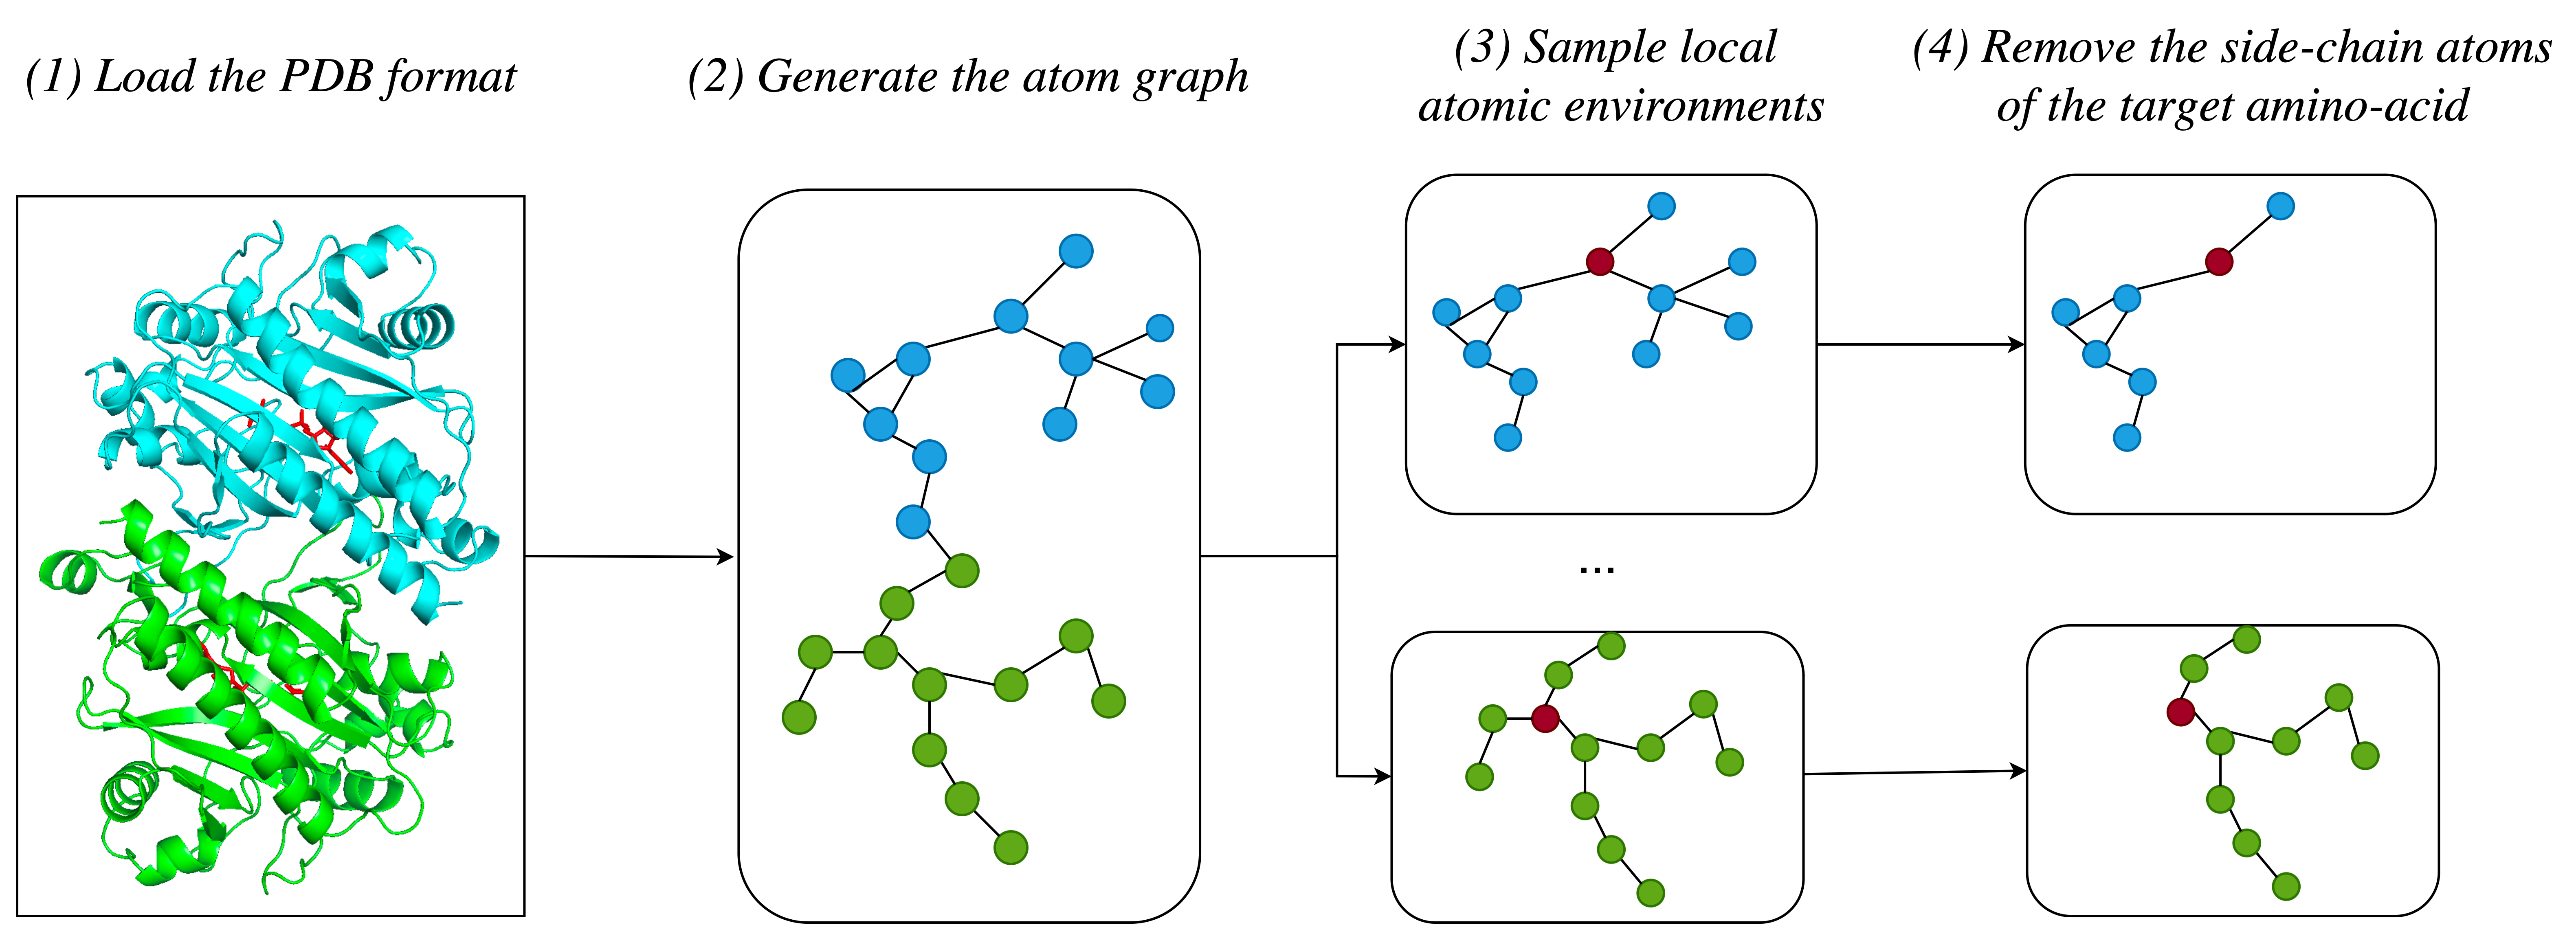
\includegraphics[width=\textwidth]{masters-report/figures/graph-pipeline.png}
    \caption{Data generation pipeline for the RES task. The local atomic environments are sampled according to indices provided by the ATOM3D dataset \cite{atom-3d}. The red nodes represent the $\text{C}_{\alpha}$ carbons of their respective amino acid residues; these are the nodes we are interested in classifying correctly.}
    \label{protein_pipeline}
\end{figure}

\paragraph{Side-chain masking.} As mentioned in Section \ref{amino-acids}, all amino acid residues share the same underlying \textit{backbone} structure. Due to this reason, when masking the target amino acid, the authors of the RES dataset only remove its \textit{side-chain} atoms. The side-chain is always bound to the $\text{C}_{\alpha}$ atom of the residue (as explained in Section \ref{amino-acids}), so we train the ML model to classify this atom as one of the 20 naturally occurring amino acids.


\paragraph{Dataset splitting and class imbalances.}
Many molecules have common ancestors, and CATH topology classes \cite{Dawson2017CATH} were introduced in order to group these protein domains into superfamilies when there is sufficient evidence they have diverged from a common ancestor. The creators of the ATOM3D RES dataset split the train, validation and test datasets such that proteins belonging to topology classes that appear in the training set will not appear in the test set. This is done as a way to properly assess the generalisation performance of the models, since otherwise the models can memorise the general attributes of a certain CATH class. 

Moreover, not all amino acids appear with the same frequency in real-life molecules. To deal with possible class imbalances, the authors downsample the local environments of the training set to the frequency of the least common amino acid (cysteine). Table \ref{dataset_stats} provides a summary of the statistics of the full RES ATOM3D dataset.


\begin{table}[]
    \centering
    \begin{tabular}{@{}lccc@{}}
    \toprule
    Dataset    & No. molecules & Avg no. samples/molecule & Avg no. atoms/sample \\ \midrule
    Train      & 21072           & 181                       & 622                   \\
    Validation & 962             & 199                       & 612                   \\
    Test       & 3303            & 196                       & 613                   \\ \bottomrule
    \end{tabular}
    \caption{Statistics of the ATOM3D RES dataset.}
    \label{dataset_stats}
\end{table}

\subsection{Training overview}
\label{training-overview}
The training pipeline is summarised in Figure \ref{res-task}. We treat this task as a node classification task, and train the model to predict the most likely side-chain for a target $\text{C}_{\alpha}$ atom given its local environment.

\begin{figure}[!h]
    \centering
    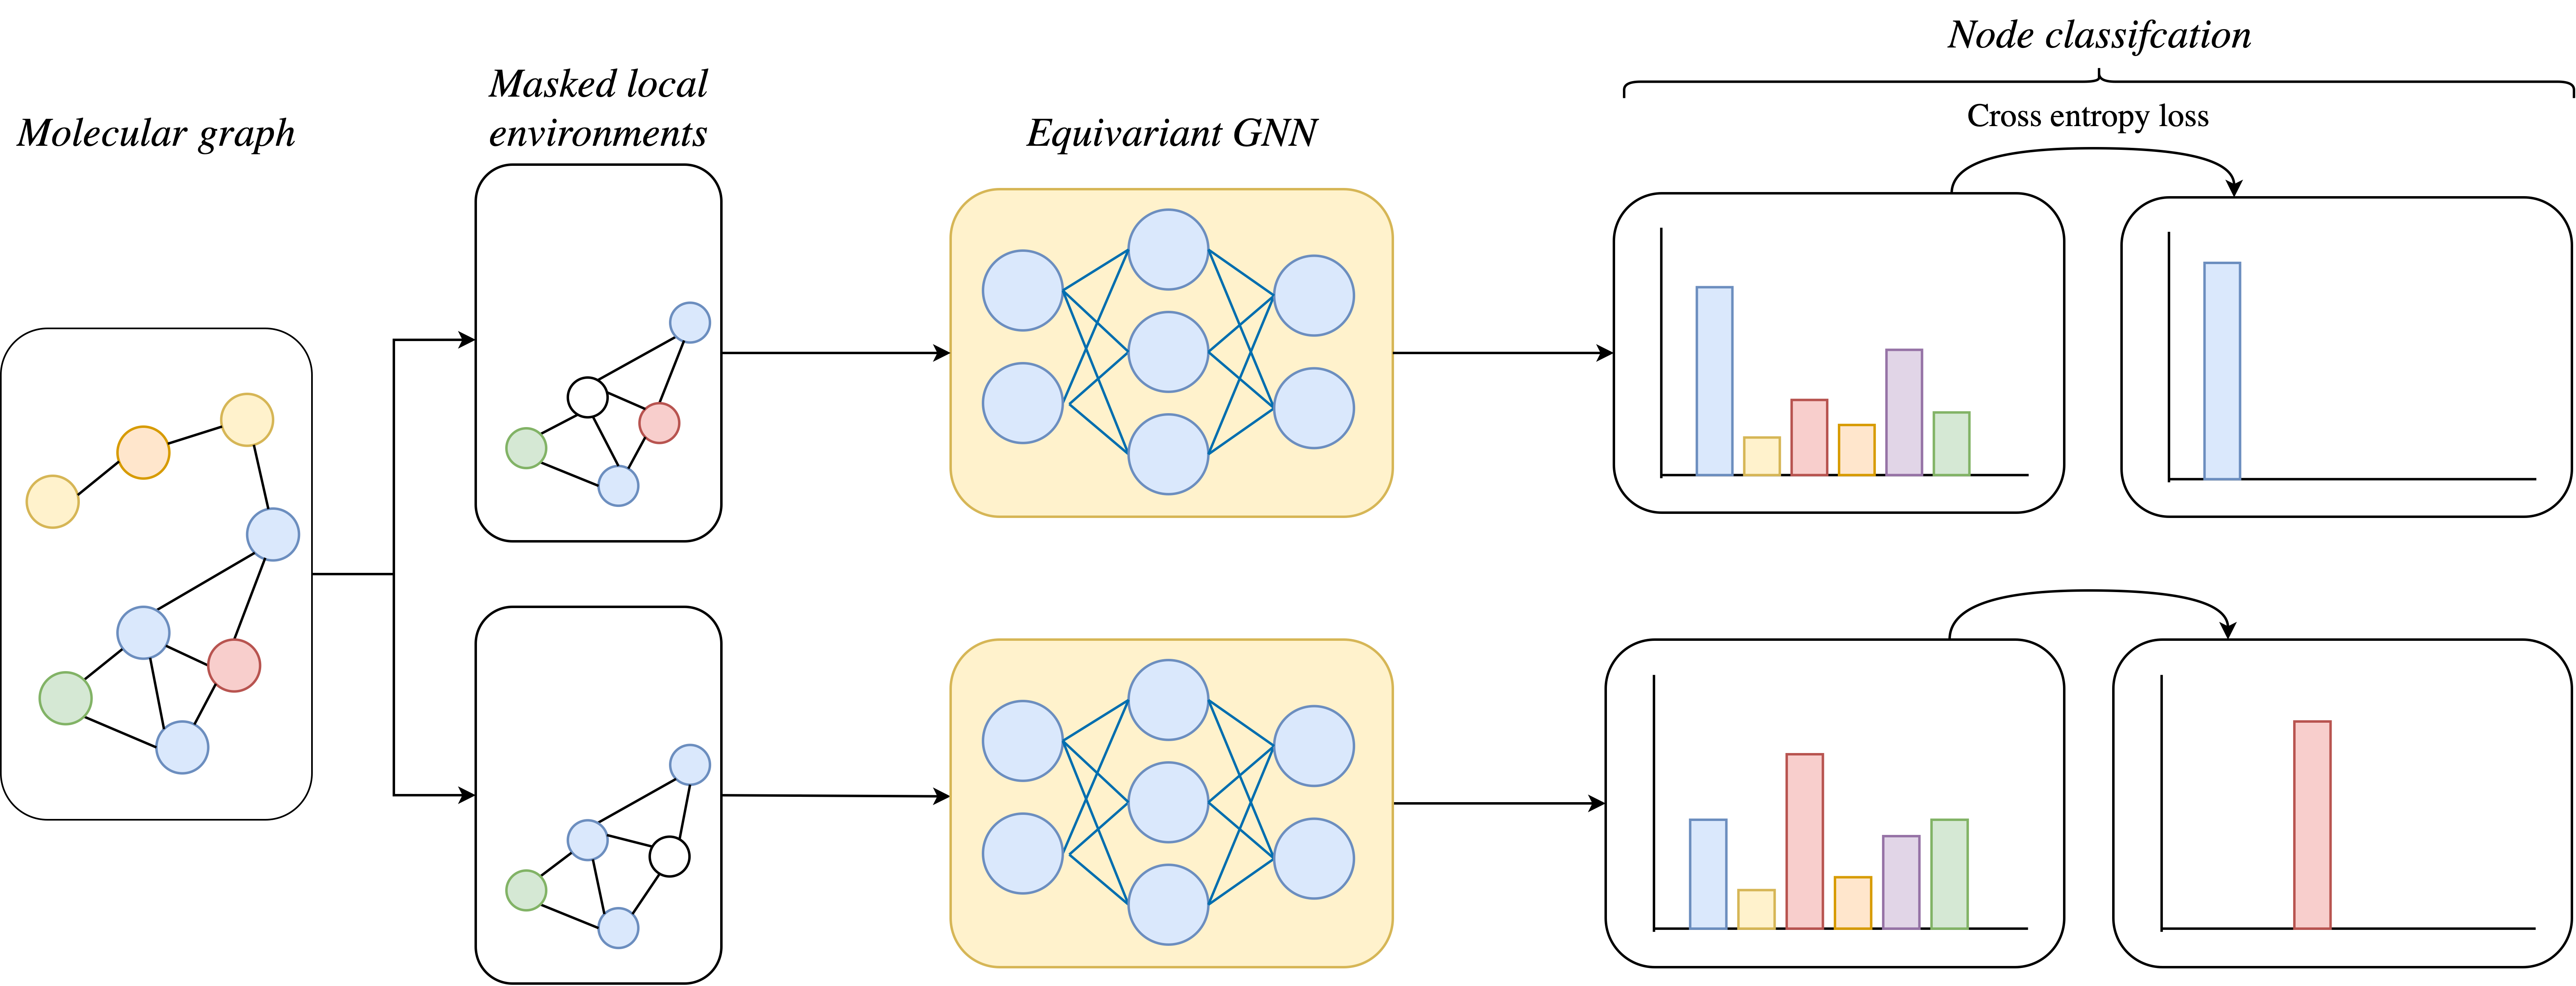
\includegraphics[width=\textwidth]{masters-report/figures/training-pipeline.png}
    \caption{Diagram of phase 1, illustrating the pipeline used in training the models on the RES task.}
    \label{res-task}
\end{figure}
\paragraph{Graph readout.} More formally, for a given graph $\mathcal{G} = (\mathcal{V}, \mathcal{E})$ with nodes $i,j \in \mathcal{V}$ and edges $(i \rightarrow j) \in \mathcal{E}$ for which we have initial scalar and vector node features $\mathbf{H}\in\mathbb{R}^{|\mathcal{V}|\times n}\times\mathbb{R}^{|\mathcal{V}|\times 3 \times \nu}$, as well as scalar and vector edge features $\mathbf{E}\in\mathbb{R}^{|\mathcal{E}|\times m}\times\mathbb{R}^{|\mathcal{E}|\times 3 \times \eta}$, we first consider a \textit{masked} version of this graph, $\mathcal{G}_t=(\mathcal{V}_t, \mathcal{E}_t)$, from which we have removed all the atoms of the side-chain attached to the node $t$ (representing an $\text{C}_{\alpha}$ atom). 

We then formally define the GNN model $\mathbf{G}_{\theta_1}:\mathbb{R}^{|\mathcal{V}_t|\times n}\times\mathbb{R}^{|\mathcal{V}_t|\times 3 \times \nu}\times\mathbb{R}^{|\mathcal{E}_t|\times m}\times\mathbb{R}^{|\mathcal{E}_t|\times 3 \times \eta}\rightarrow \mathbb{R}^{|\mathcal{V}_t|\times o}$ that takes as input the node and edge features and returns final node features  $\mathbf{H}_{\text{out}}$:
\begin{equation}
    \mathbf{H}_{\text{out}} = \mathbf{G}_{\theta_1}(\mathbf{H}_t, \mathbf{E}_t)
\end{equation}
where $\mathbf{H}_t$ and $\mathbf{E}_t$ represent the node and edge features for all nodes and edges that exist in the masked graph $\mathcal{G}_t$.

Since we are interested in predicting the type of amino acid corresponding to the masked side-chain of node $t$, we define a pooling function $\text{pool}:\mathbb{N}\times\mathbb{R}^{|\mathcal{V}_t|\times o}\rightarrow \mathbb{R}^o$ that retrieves the final features of node $t$:
\begin{equation}
    \text{pool}(t, \mathbf{H}_{\text{out}}) = [\mathbf{H}_{\text{out}}]_t
\end{equation}

We pass $\mathbf{h}_{t} = \text{pool}(t, \mathbf{H}_{\text{out}})$ through a multi-layer perceptron $\text{MLP}_{\theta_2}:\mathbb{R}^o\rightarrow \mathbb{R}^{20}$ to obtain the final scores associated to each of the 20 naturally occuring amino acids:
\begin{equation}
    l = \text{MLP}_{\theta_2}(\mathbf{h}_t)
\label{logit-scores}
\end{equation}
Hence, the masking process, the overall GNN model, and the downstream MLP form the node classification function $f_{\gamma}^t:\mathbb{R}^{|\mathcal{V}|\times n}\times\mathbb{R}^{|\mathcal{V}|\times 3 \times \nu}\times\mathbb{R}^{|\mathcal{E}|\times m}\times\mathbb{R}^{|\mathcal{E}|\times 3 \times \eta}\rightarrow \mathbb{R}^{20}$ with learnable parameters $\gamma = \{\theta_1, \theta_2\}$:
\begin{equation}
    f_{\gamma}^t(\mathbf{H}, \mathbf{E}) = \text{MLP}_{\theta_2}(\text{pool}(t, \mathbf{G}_{\theta_1}(\mathbf{H}_t, \mathbf{E}_t)))
\label{full-formalism}
\end{equation}

The \textbf{loss function} of our model quantifies the dissimilarity between the predicted probability distribution associated with scores $l$ obtained in Equation \ref{logit-scores} and the true probability distribution associated with the target class, also known in the literature as the cross-entropy loss:
\begin{equation}
    \mathcal{L}(l, y) = -\log\frac{\exp({l_y})}{\sum_{c=1}^{20} \exp({l_c})}
\label{logits}
\end{equation}
where $y \in \{1,2,\dots,20\}$ is the true class of target node $t$.
\subsection{The geometric vector perceptron}
\label{the-gvp-math}
The first of the two architectures employed for pre-training in this project is the Geometric Vector Perceptron (GVP). The GVP is an equivariant learning module introduced by \citet{gvp1}. It lays the foundation for the GVP-GNN model, an equivariant GNN that has proven to be a successful architecture for many structure-based molecular tasks \cite{gvp1, gvp2}. In this work, we are using the second version of the GVP-GNN architecture, as described in \citet{gvp2}. 

\paragraph{The GVP module.}
The GVP module can learn both scalar-valued and vector-valued functions over geometric vectors and scalars; it can be thought of as generalising the concept of a Multi-Layer Perceptron to vectors, hence its ability to learn geometric properties of molecules. 

Borrowing some notation from \citet{gvp1}, for each node in a graph we can define the tuple $\mathbf{h} = (\mathbf{s}, \mathbf{V})$ of scalar features $\mathbf{s}\in\mathbb{R}^{n}$ and vector features $\mathbf{V}\in \mathbb{R}^{\nu\times 3}$. Then, the GVP computes updated features $\mathbf{h}'=(\mathbf{s}', \mathbf{V}') \in \mathbb{R}^m\times\mathbb{R}^{\mu \times 3}$ as can be seen in Algorithm \ref{gvp-algo}.
\begin{figure}[!h]
    \begin{minipage}[b]{0.3\textwidth}
    \centering
    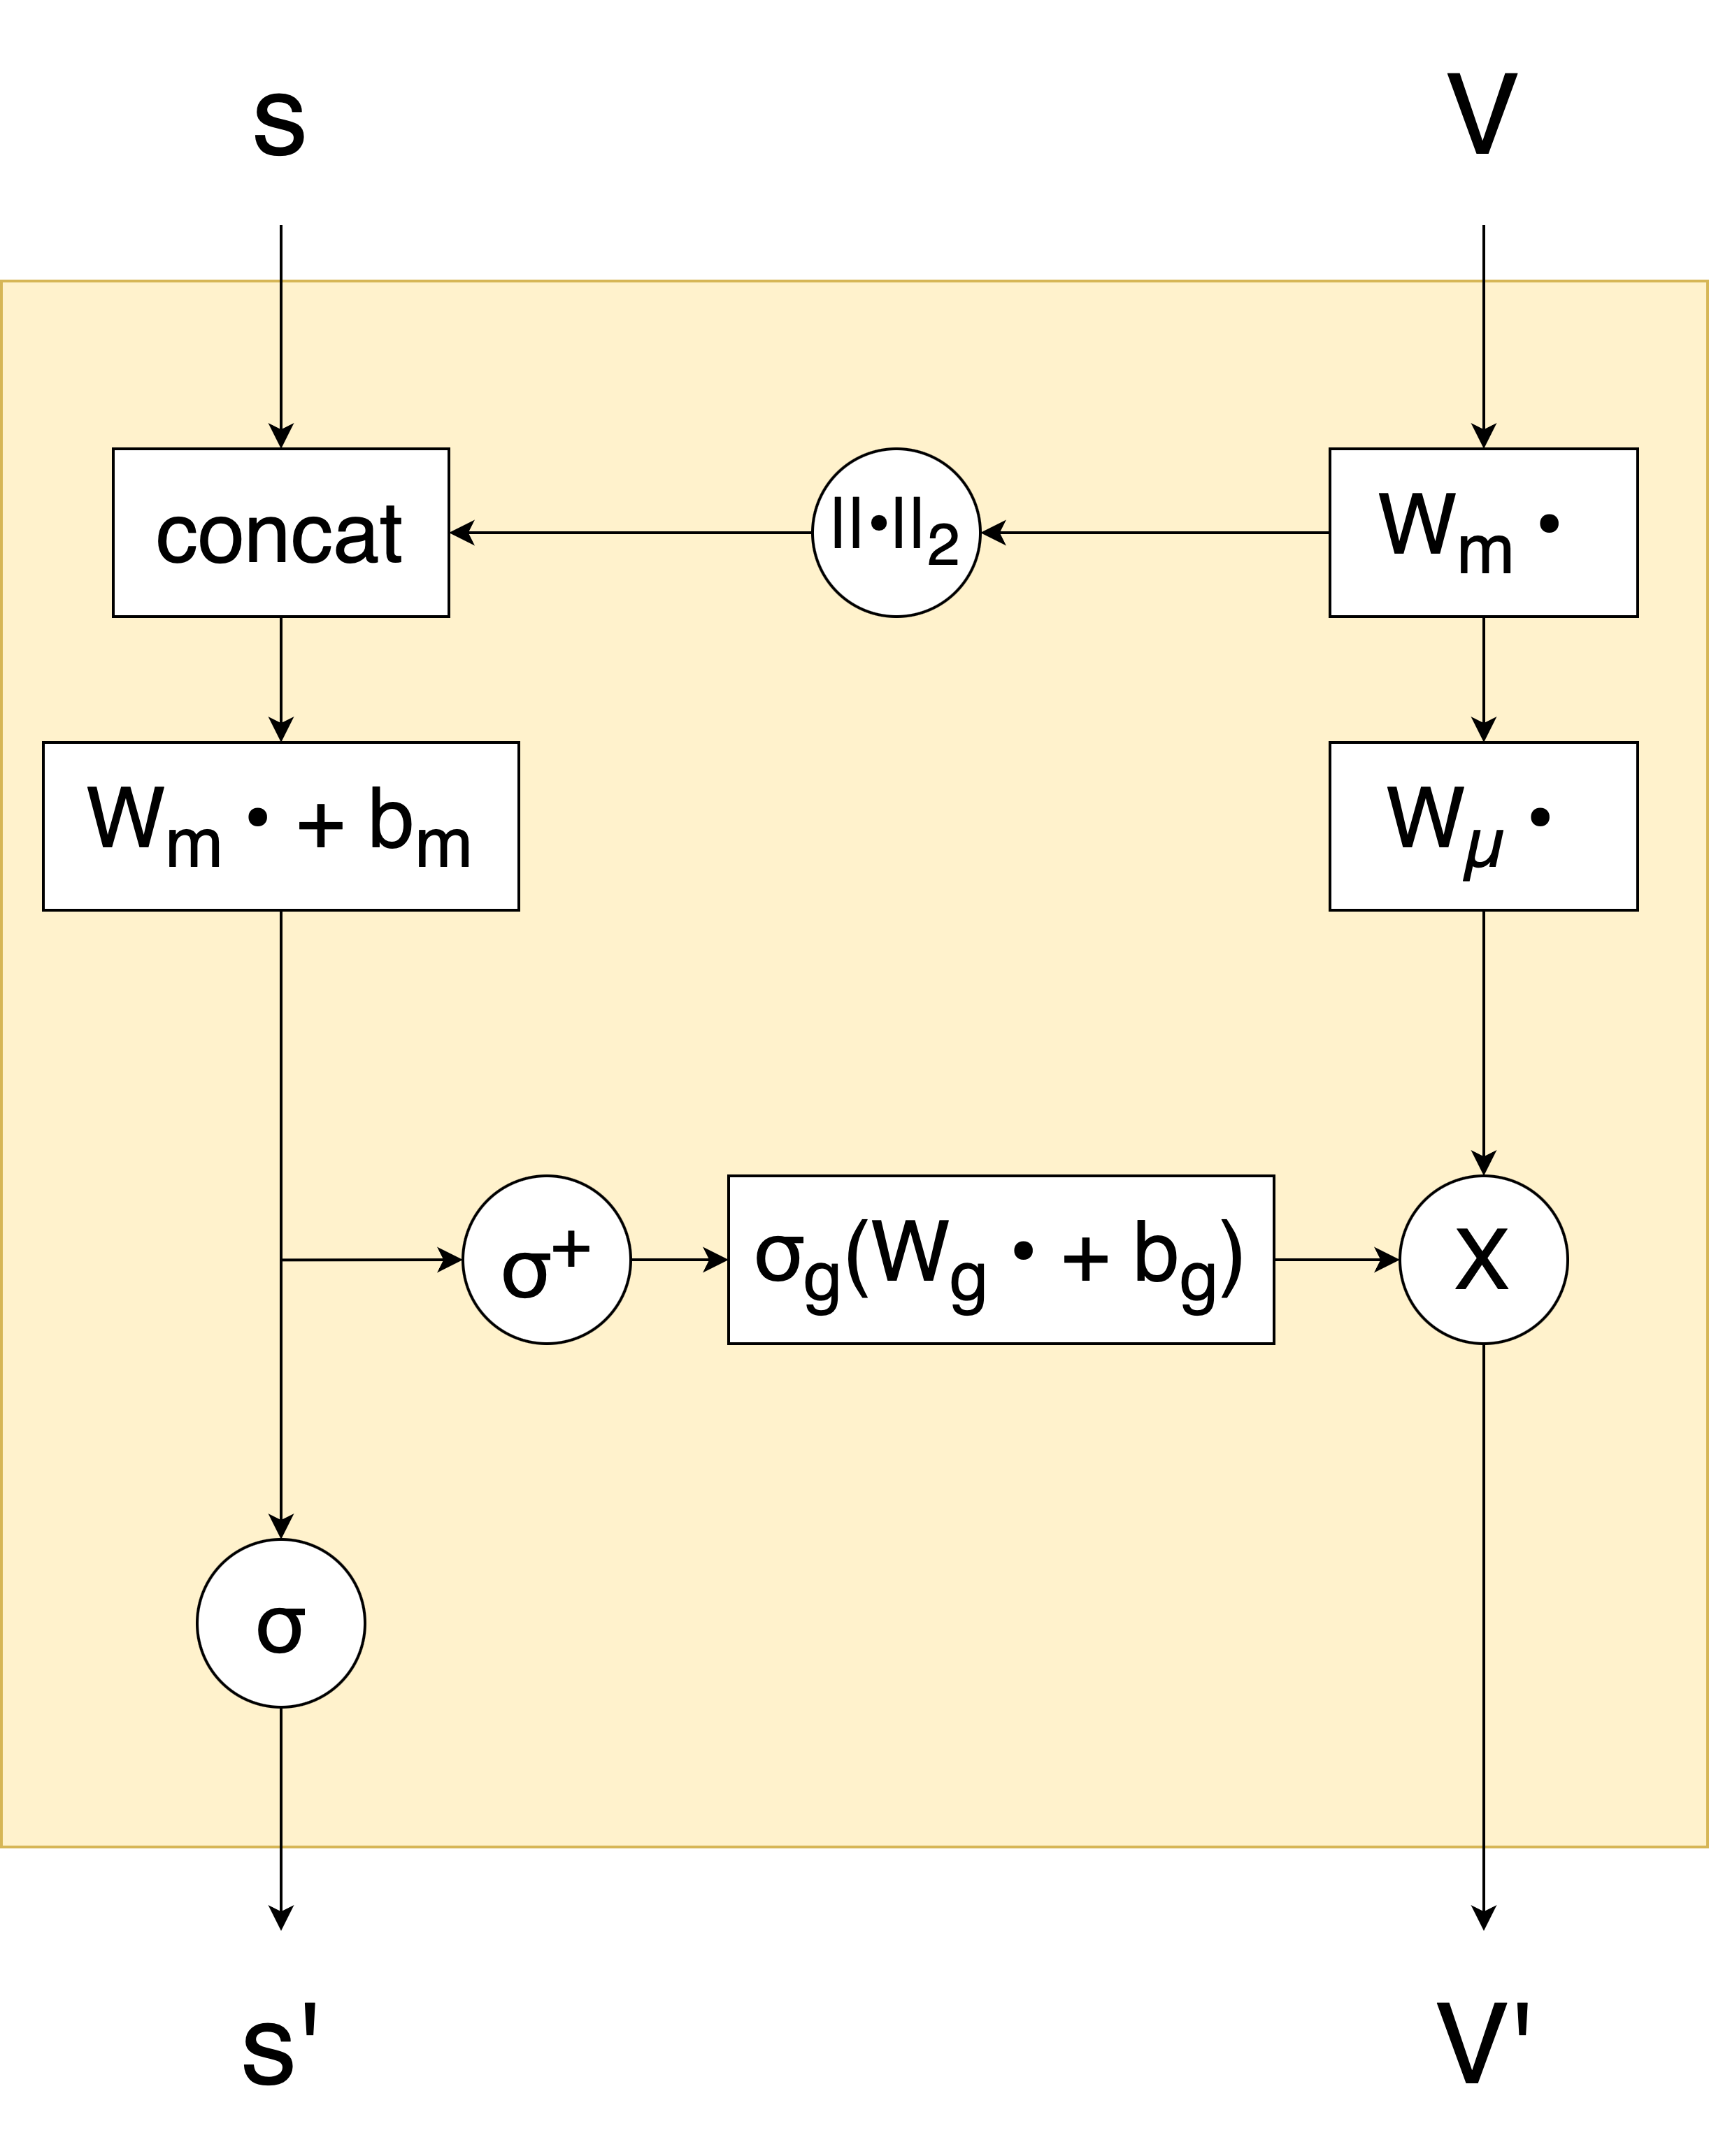
\includegraphics[width=\textwidth]{masters-report/figures/gvp.png}
    \label{fig:image}
  \end{minipage}
  \hfill
  \begin{minipage}[b]{0.65\textwidth}
    % \begin{algorithm}
% \caption{Geometric Vector Perceptron}
\hline
\begin{algorithmic}
\renewcommand{\algorithmicrequire}{\textbf{Input:}}
\renewcommand{\algorithmicensure}{\textbf{Output:}}
\Require{Scalar and vector feats. $(\mathbf{s}, \mathbf{V}) \in \mathbb{R}^n\times \mathbb{R}^{\nu \times 3}$}
\Ensure{Scalar and vector feats. $(\mathbf{s}', \mathbf{V}')\in \mathbb{R}^n\times\mathbb{R}^{\mu\times 3}$}
\State $h \gets \max(\nu, \mu)$

\State $V_h \gets \mathbf{W}_h\mathbf{V} \in \mathbb{R}^{h\times3}$

\State $V_{\mu} \gets \mathbf{W}_{\mu}\mathbf{V}_h \in \mathbb{R}^{\mu\times 3}$

\State $\mathbf{s}_h\gets ||V_h||_2$ (row-wise) $\in \mathbb{R}^h$

\State $\mathbf{v}_{\mu} \gets ||V_{\mu}||_2$ (row-wise) $\in \mathbb{R}^{\mu}$

\State $\mathbf{s}_{h + n} \gets \text{concat}(\mathbf{s}_h, \mathbf{s})\in\mathbb{R}^{h + n}$

\State $\mathbf{s}_m \gets \mathbf{W}_m\mathbf{s}_{h+n}+\mathbf{b}\in \mathbb{R}^m$

\State $\mathbf{s}' \gets \sigma(\mathbf{s}_m)\in \mathbb{R}^m $

\State $\mathbf{V}' \gets \sigma_g(\mathbf{W}_g[\sigma^{+}(\mathbf{s}_m)] + \mathbf{b}_g) \circledcirc \mathbf{V}_{\mu}$ (row-wise) $\in \mathbb{R}^{\mu \times 3}$
\\
\Return $(\mathbf{s}', \mathbf{V}')$
\end{algorithmic}
\hline
% \end{algorithm}

  \end{minipage}
\caption{\textit{(Left)} An illustration of the data flow of the module; \textit{(Right)} Algorithm showing the computation involved in a GVP module.  Both the pseudocode and the illustration are adapted from \cite{gvp2}.}
\label{gvp-algo}
\end{figure}

\paragraph{The message-passing framework.} The GVP module can be incorporated in the message-passing framework to create a \textit{GVP convolutional layer}. If $\mathbf{h}_{\mathcal{V}}^{(j)}$ are the node features of node $j$ and $\mathbf{h}_{\mathcal{E}}^{(j\rightarrow i)}$ are the edge features of edge $(j \rightarrow i)$, then the module creates the message $\mathbf{m}^{(j\rightarrow i)}$ passed from node $j$ to node $i$ as follows:
\begin{equation}
\mathbf{m}^{(j\rightarrow i)} = g_1\Big(\text{concat}(\mathbf{h}_{\mathcal{V}}^{(j)}, ~~\mathbf{h}_{\mathcal{E}}^{(j \rightarrow i)})\Big) 
\end{equation}
Assuming $k$ is the number of incoming messages, we aggregate them according to:
\begin{equation}
\mathbf{m}_{\mathcal{V}}^{(i)}= \text{LayerNorm}\Big(\mathbf{h}_{\mathcal{V}}^{(i)} + \frac{1}{k}\text{Dropout}\big(\sum_{(j \rightarrow i)\in\mathcal{E}}\mathbf{m}^{(j\rightarrow i)}\big)\Big)
\label{aggregation}
\end{equation}
We follow this with a \textit{feed-forward point-wise} layer to update the node embeddings:
\begin{equation}
    \mathbf{h}_{\mathcal{V}}^{(i)}= \text{LayerNorm}\Big(\mathbf{m}_{\mathcal{V}}^{(i)} + \text{Dropout}\big(g_2(\mathbf{m}_{\mathcal{V}}^{(i)})\big)\Big)
\label{update}
\end{equation}
Functions $g_1$ and $g_2$ are compositions of three and two GVP modules, respectively.

\paragraph{Layer normalisation and dropout.} Dropout \cite{dropout} is a regularisation technique that randomly ``drops out'' a portion of the neurons during training, while layer normalisation \cite{layernorm} is a technique that normalises the activations of neurons within a layer to address the problem of internal covariate shift. Both techniques are widely used in practice to avoid overfitting. 

When dealing with scalar features, the equations \ref{aggregation} and \ref{update} use the standard implementations of these two layers. However, when dealing with vector features, \citet{gvp1} modify the Dropout layer to ``drop'' entire 3D vectors. Additionally, they define layer normalisation for vector features to scale the row vectors of $\mathbf{V} =[\mathbf{v}_1, \dots, \mathbf{v}_{\nu}]$, where $\nu$ is the number of vector features per node, such that the root-mean-square norm is equal to 1: 
\begin{equation}
    \mathbf{V} \leftarrow \mathbf{V}/\sqrt{\frac{1}{\nu}||\mathbf{V}||_2^2} ~~\in \mathbb{R}^{\nu\times 3}  
\end{equation}


The final architecture is composed of GVP modules, layer normalisation modules and GVP convolutional layers, as illustrated in Figure \ref{gvp-architecture}.
\begin{figure}
    \centering
    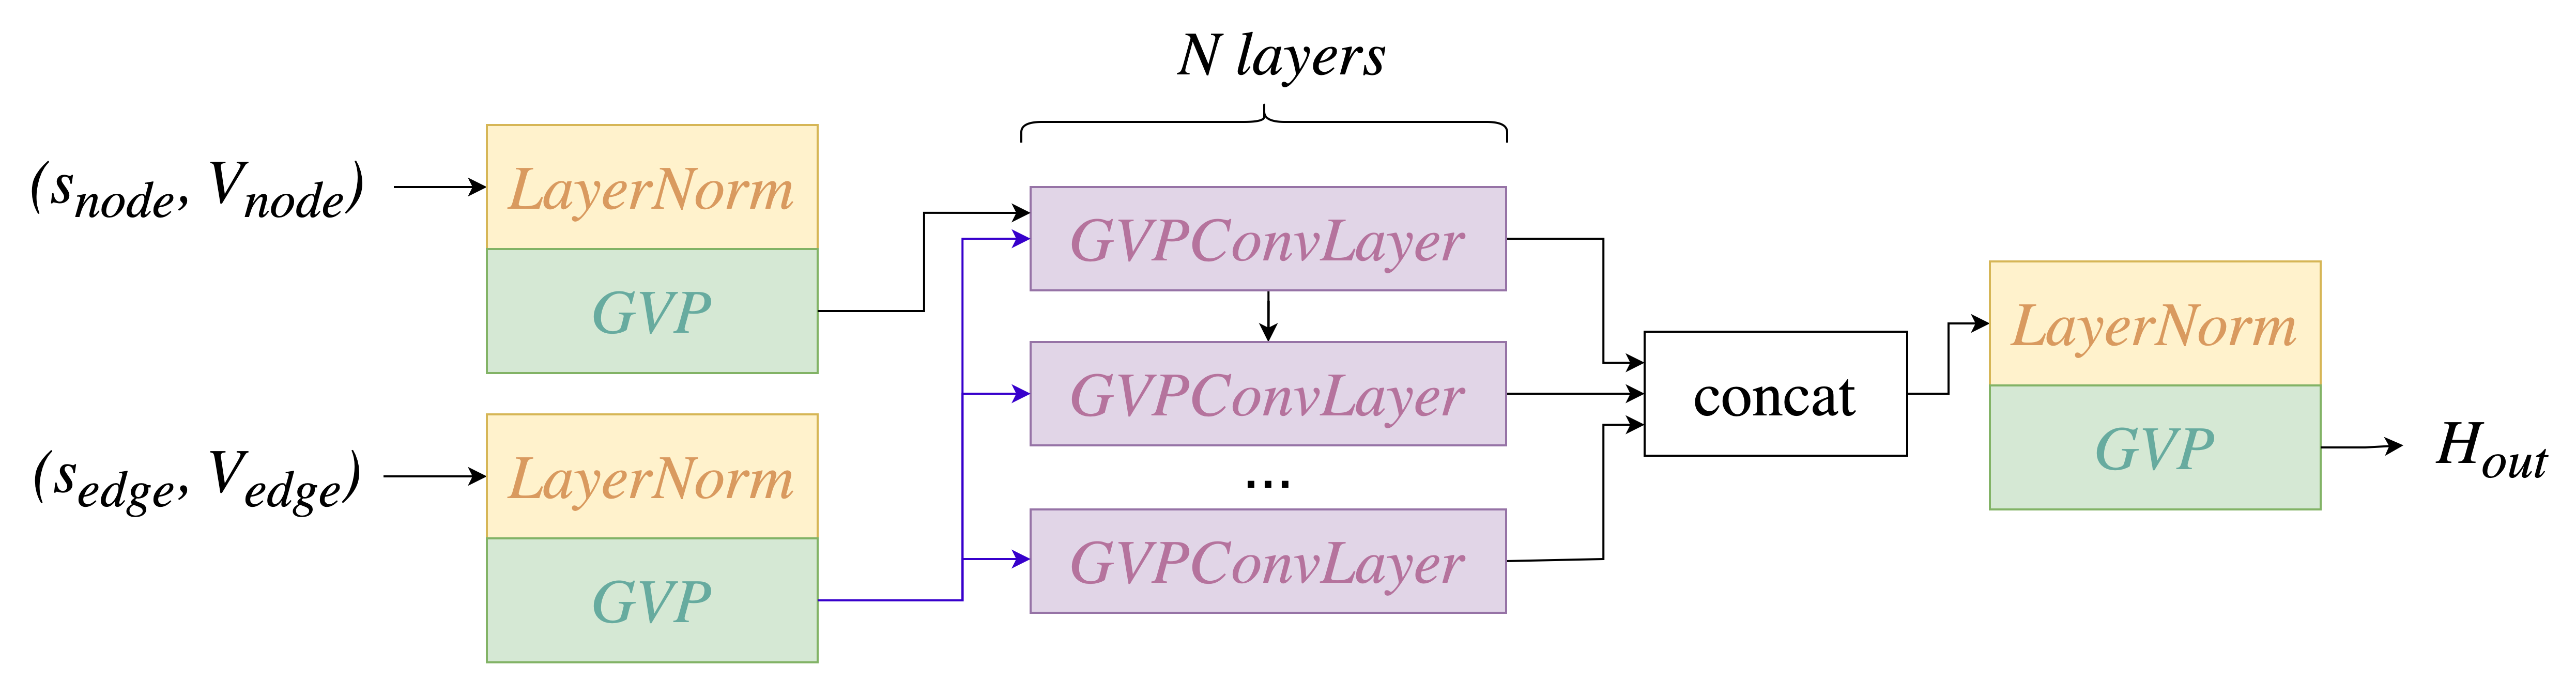
\includegraphics[width=\textwidth]{masters-report/figures/gvp-architecture.png}
    \caption{Overall architecture of the GVP-GNN model.}
    \label{gvp-architecture}
\end{figure}

\paragraph{Initial features.} 
The initial features used on the GVP-GNN architecture are separated into node features $(\mathbf{s}_{\text{node}}, \mathbf{V}_{\text{node}})$ and edge features $(\mathbf{s}_{\text{edge}}, \mathbf{V}_{\text{edge}})$. We obtain the scalar node features by passing its node type $z_{\text{node}}$ through a trainable embedding layer to obtain $\mathbf{s}_{\text{node}} = \text{embed}(z_{\text{node}})$, where $\text{embed}:\mathcal{A}\rightarrow \mathbb{R}^n$. All of the initial node vector features $\mathbf{V}_{\text{node}}$ are set to $\vec{\mathbf{0}}$.

To obtain the scalar edge features $\mathbf{s}_{\text{edge}}$, for each edge from node $i$ to node $j$ we encode the interatomic distance $d_{ji}$ in terms of Gaussian radial basis functions (RBFs). The reason for encoding the distance using RBFs is that these functions are non-zero only within a specified radius. This property enables them to capture local interactions between atoms while minimising the influence of distant nodes. Using these encodings instead of the plain Euclidean distance allows the model to learn how to treat different length scales in separate manners.

More formally, for hyperparameter $\epsilon\in\mathbb{R}_{+}$ controlling the smoothness of the basis function, we define the encoding of $d_{ji}$ to be:
\begin{equation}
    \text{GBF}_{\epsilon}(d_{ji}) = e^{-(\epsilon d_{ji})^2}
\end{equation}
I use 16 different $\epsilon$ values, evenly spaced between 0 to 20, rendering the final scalar edge features $\mathbf{s}_{ij} \in \mathbb{R}^{16}$. For the vector edge embeddings I compute the normalised edge direction: $\vec{\mathbf{v}}_{ij} = \frac{\mathbf{p}_i - \mathbf{p}_j}{||\mathbf{p}_i - \mathbf{p}_j||_2}$. 

\subsection{The equivariant graph attention network}
\label{eqgat-math}
The second EGNN architecture used in this project is the equivariant graph attention network introduced by \citet{eqgat}. A brief introduction into self-attention mechanisms is presented before diving into the specifics of this EGNN model.

Attention in neural networks refers to a mechanism that enables the network to focus on specific parts of the input data or relevant information while processing a task. It is inspired by human attention and aims to improve the network's ability to handle long sequences or complex patterns. The most popular attention mechanism to date was introduced by \citet{vaswani2017attention} and lies at the core of the Transformer architecture. 

The attention mechanism typically involves two components: a \textbf{query} and a set of \textbf{key-value pairs}. The query represents the information the network is currently processing, while the key-value pairs represent the contextual information or memory. The attention mechanism computes the similarity between the query and the keys to obtain \textit{attention weights}, which determine the importance of each value. Figure \ref{attention} illustrates the conceptual pipeline of a self-attention module.

\begin{figure}[!h]
    \centering
    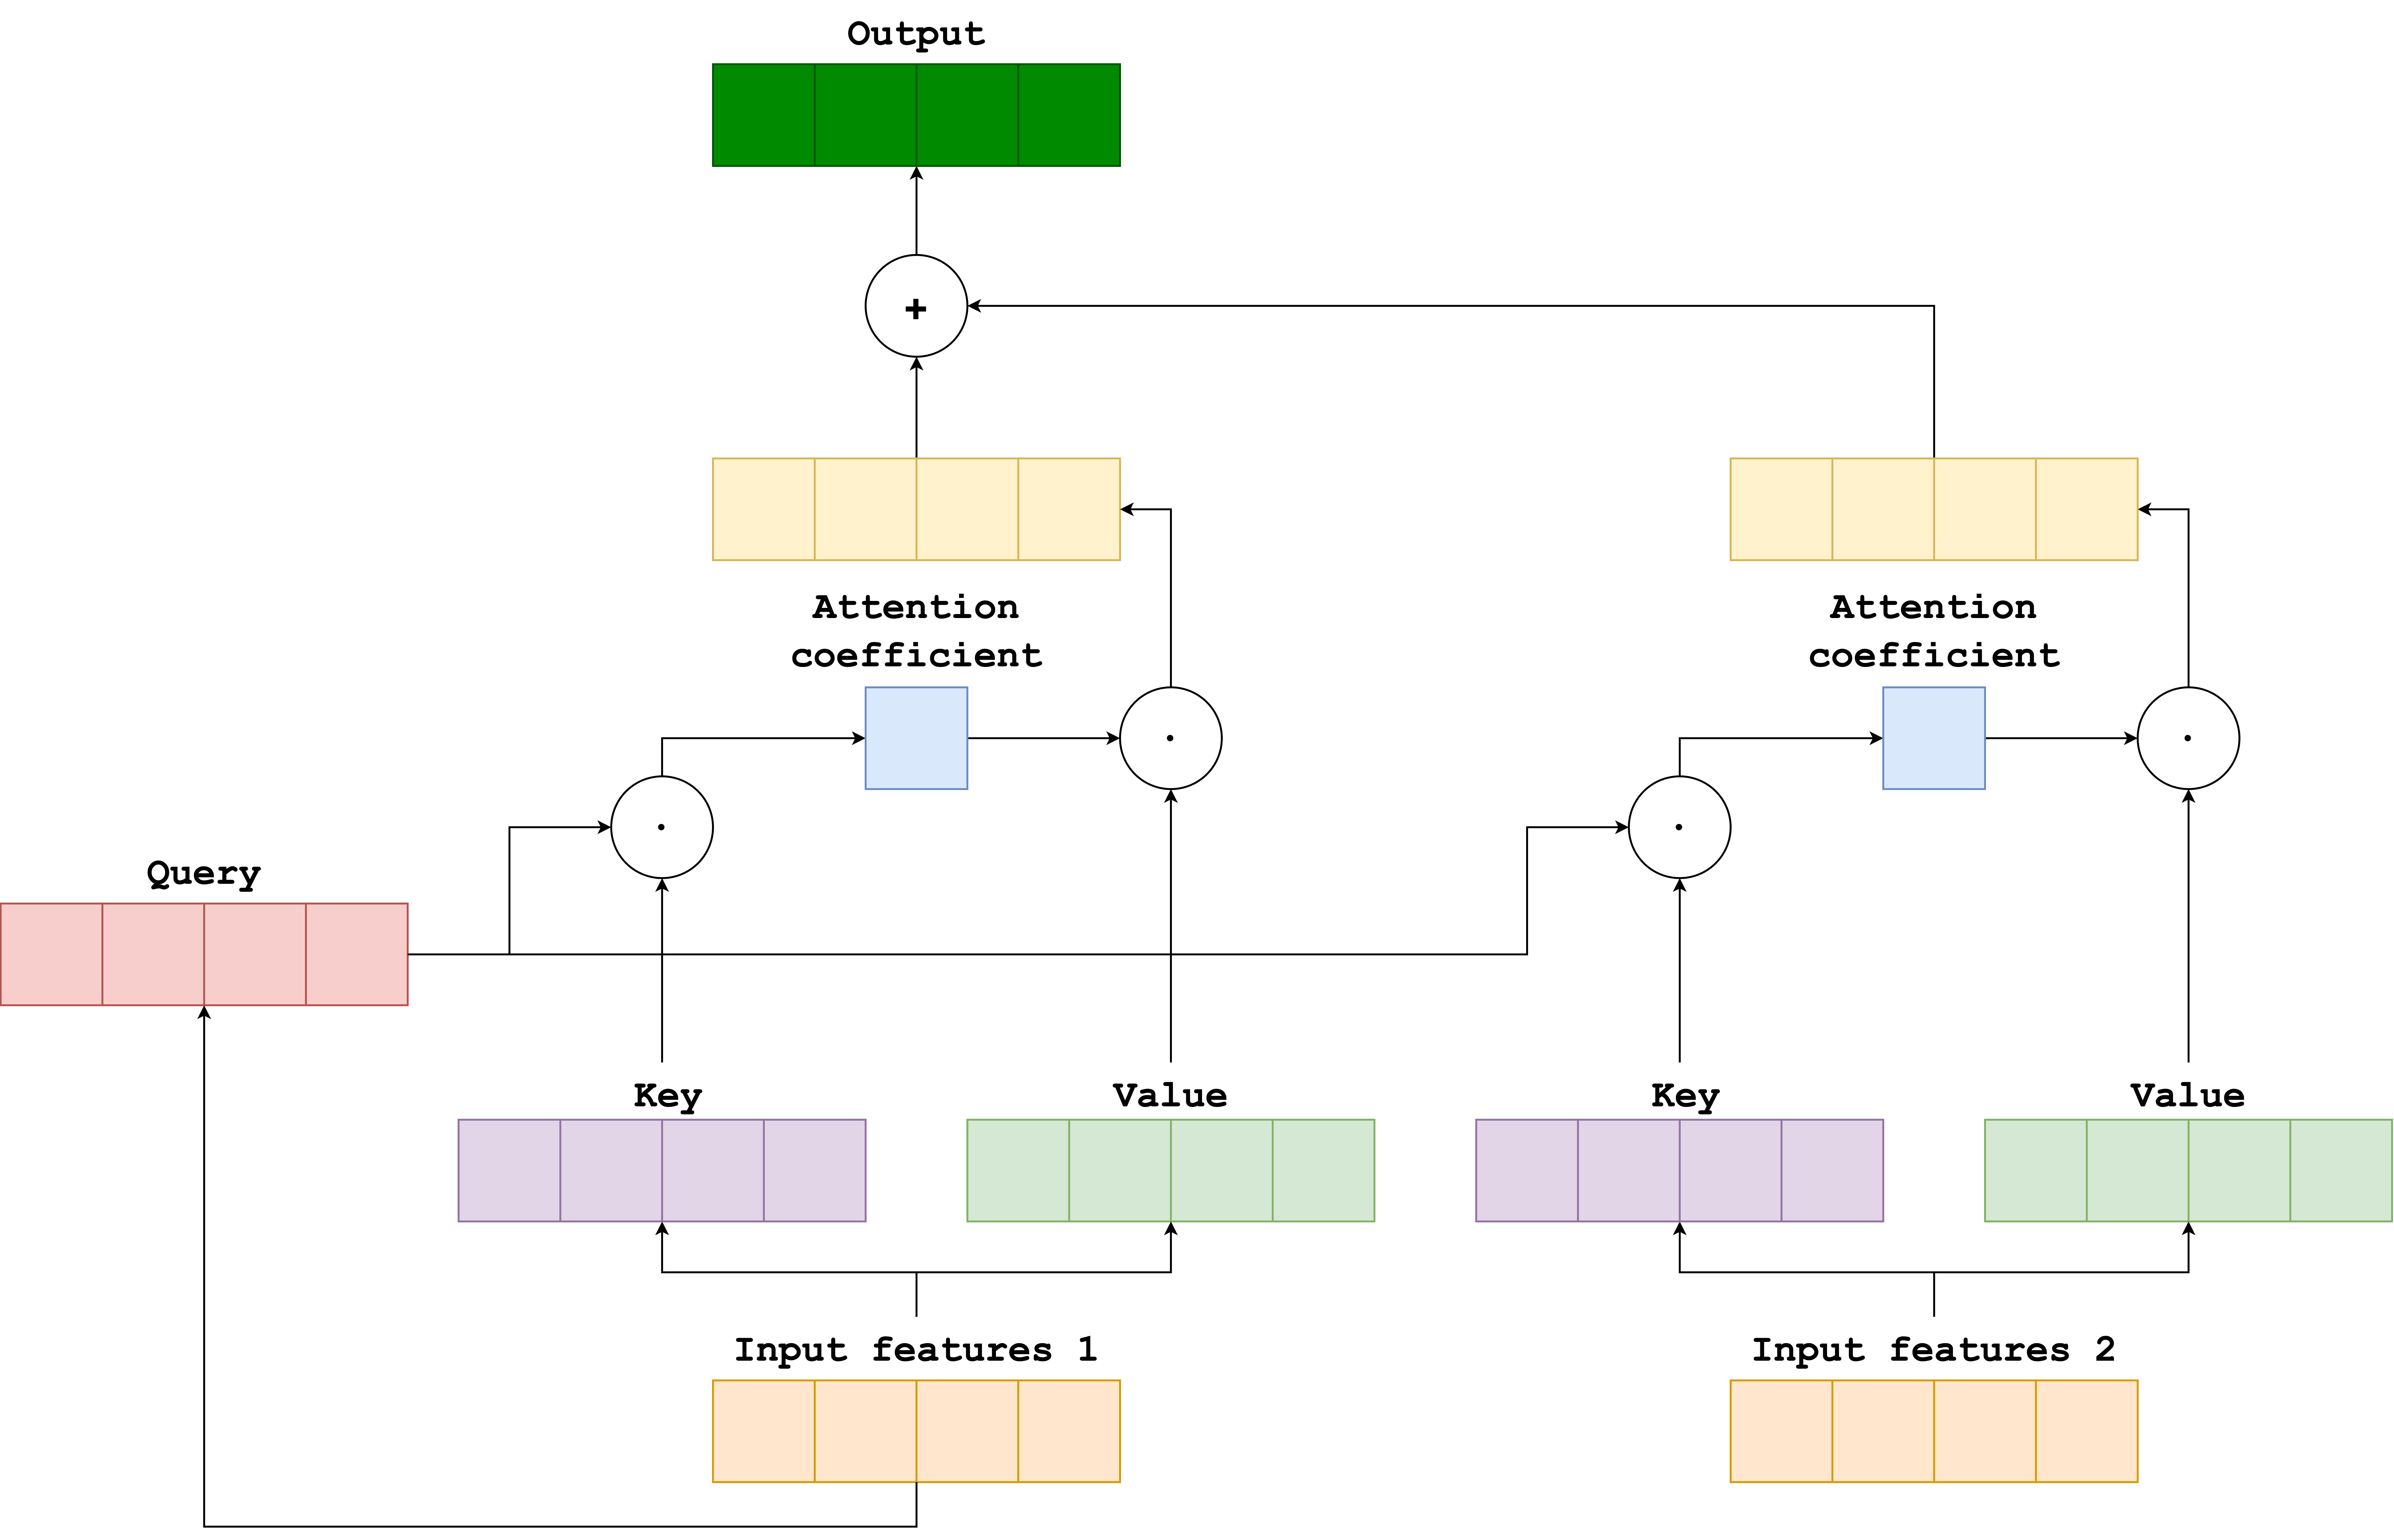
\includegraphics[width=0.8\textwidth]{masters-report/figures/attention-mechanism.png}
    \caption{Overall idea of the self-attention mechanism used in \citet{vaswani2017attention}. Note that the operation that combines the key and the query is highly dependent on the architecture used; for the sake of simplicity, I illustrate the scalar dot product.}
    \label{attention}
\end{figure}

\citet{gat} expanded the attention principle to the realm of GNNs by introducing \text{Graph Attention Networks} (GATs). The attention mechanism proposed by the authors allows the model to focus on different neighbours of a node while aggregating information from its neighbourhood. It assigns attention weights to the neighboring nodes based on their relevance to the target node. The attention weights are learned during the training process and reflect the importance of each neighbour for the target node.

In this work, we are using a version of the GAT network that applies the \textit{self-attention} principle to both scalar and geometric features, allowing the model to learn structural information. \citet{eqgat} propose the \textbf{Equivariant Graph Attention Network} (EQGAT), a model that is equivariant to 3D rotations and translations.

\paragraph{The attention mechanism.} Using a similar notation to the one in Section \ref{the-gvp-math}, for a graph $\mathcal{G} = (\mathcal{V}, \mathcal{E})$, given two nodes $i, j \in \mathcal{V}$ with scalar features $\mathbf{h}_i, \mathbf{h}_j \in \mathbb{R}^{n}$ and edge vector features $\mathbf{e}_{ji}\in \mathbb{R}^n$, we first compute the \textit{query} and \textit{key} vectors by passing the features through two linear layers:
\begin{align}
    \mathbf{q}_i &= \mathbf{W}_q\mathbf{h}_i + \mathbf{b}_q \in \mathbb{R}^n\\
    \mathbf{k}_j &= \mathbf{W}_k\mathbf{h}_j + \mathbf{b}_k \in \mathbb{R}^n
\end{align}
We then take the element-wise product of the key, query and edge features and apply a linear transformation to it to retrieve a vector of attention coefficients $\mathbf{a}_{ji} \in \mathbb{R}^{n + 2\nu}$:
\begin{align}
    \mathbf{\Tilde{a}} &= \mathbf{q}_i \odot \mathbf{k}_j \odot \mathbf{e}_{ji} \\
    \mathbf{a}_{ji} &= \mathbf{W}_a\mathbf{\Tilde{a}}_{ji} = [\Tilde{\mathbf{\alpha}}_{ji}, \mathbf{\beta}_{ji}, \mathbf{\gamma}_{ji}]
\label{attention-coeffs}
\end{align}
The vector $\Tilde{\mathbf{\alpha}}_{ji} \in \mathbb{R}^{n}$ is then used to compute the final attention coefficients for the \textit{scalar features} as follows:
\begin{equation}
    \mathbf{\alpha}_{ji} = \frac{\sigma(\Tilde{\mathbf{\alpha}}_{ji})}{\sum\limits_{j':(j'\rightarrow i)\in\mathcal{E}}\sigma(\Tilde{\mathbf{\alpha}}_{ji})} \in (0, 1)^{n}
\end{equation}
We then compute the \textit{value} tensors for the attention mechanism using weight matrices $\mathbf{W}_{sv}\in\mathbb{R}^{n\times (n+2\nu)}$ and $\mathbf{W}_{vv}\in\mathbb{R}^{n\times n}$:
\begin{align}
    \label{value-tensors} \mathbf{v}_{s, j} &= [\mathbf{v}_{s_0}, \mathbf{y}_{v_0, j}, \mathbf{y}_{v_1, j}] = \mathbf{W}_{sv}\mathbf{h}_j + \mathbf{b}_{sv}  
    \\ \vec{\mathbf{v}}_{v, j} &= \vec{\mathbf{v}}_j\mathbf{W}_{vv}
\end{align}

Finally, we extend the attention mechanism to the vector features. Given that we have initial vector features $\vec{\mathbf{v}}_i, \vec{\mathbf{v}}_j$ for nodes $i$ and $j$, we create vector attention coefficient $\vec{\mathbf{a}}_{v, ji}$ as follows:
\begin{equation}
    \vec{\mathbf{a}}_{v, ji} = \vec{\mathbf{v}}_j \times \vec{\mathbf{v}}_i + \vec{\mathbf{v}}_{v, j}
\end{equation}

\paragraph{Message construction.}
Once we have constructed all necessary features for the attention mechanism, we can compute the incoming messages for the message-passing framework. First, the scalar message from node $j$ to node $i$ is computed as:
\begin{equation}
    \mathbf{m}_{s, ji} = \mathbf{\alpha}_{ji}\odot\mathbf{v}_{s_0, j}
\end{equation}
Next, we compute two types of vector messages from node $j$ to node $i$ using the coefficients computed in Equation \ref{attention-coeffs} and the value tensors computed in Equation \ref{value-tensors}:
\begin{align}
    \mathbf{m}_{v_0, ji} &= \mathbf{\beta}_{ji}\odot \mathbf{y}_{v_0, j}\\
    \mathbf{m}_{v_1, ji} &= \mathbf{\gamma}_{ji}\odot \mathbf{y}_{v_1, j}    
\end{align}
We use these vector messages to construct \textit{equivariant interactions} between nodes $j$ and $i$ by using their relative position $\vec{p}_{ji} = \vec{p}_i - \vec{p}_j$ in 3D space. More formally, we obtain the normalised position $\vec{p}_{e,ij} = \frac{\vec{p}_{ij}}{||\vec{p}_{ij}||_2}$ and combine this with vector message $\mathbf{m}_{v_0,ji}\in\mathbb{R}^n$ through the cross product:
\begin{align}
    \vec{\mathbf{y}}_{0, ji} &= \vec{p}_{e,ij}\otimes\mathbf{m}_{v_0,ji} = \vec{p}_{e,ij}\mathbf{m}_{v_0, ji}^{\top} \in \mathbb{R}^{3\times\nu}
\label{position-cross-product} \\
    \vec{\mathbf{y}}_{1, ji} &= (\mathbf{1}\otimes\mathbf{m}_{v_1, ji})\odot \vec{\mathbf{a}}_{v, ji}\text{, where }\mathbf{1}\in\mathbb{R}^3
\end{align}
\paragraph{Message aggregation.}
The final aggregated message that we form for node $i$ sums the messages received from each of its neighbours on the scalar and vector channels, respectively:
\begin{align}
    \mathbf{m}_{s, i} &= \sum_{j\in\mathcal{N}(i)}\mathbf{m}_{s, ji}\\
    \mathbf{m}_{v, i} &= \sum_{j\in\mathcal{N}(i)}(\vec{\mathbf{y}}_{0, ji} + \vec{\mathbf{y}}_{1, ji}) \\
    \mathbf{m}_i &= (\mathbf{m}_{s, i}, \mathbf{m}_{v, i})
\end{align}

\paragraph{Update.} The last step within a message-passing step is the update. For the update, the authors first sum together the updated state $\mathbf{m}_i$ and the previous state $\mathbf{x}_i = (\mathbf{h}_i, \vec{\mathbf{v}}_i)$:
\begin{equation}
    \mathbf{\Tilde{x}}_i = \mathbf{x}_i + \mathbf{m}_i
\end{equation}
Notice how in this way we combine information about the node's previous state $\mathbf{x}_i\in\mathbb{R}^n\times\mathbb{R}^{3\times\nu}$ with the newly created message $\mathbf{m}_i$. The last step in this layer is to perform a pointwise update using \textit{gated equivariant non-linearities}. The update step is similar to the one in the GVP-GNN architecture and is described in Figure \ref{eqgat}(b). A diagram of the overall EQGAT architecture can be found in Figure \ref{eqgat}. 

% More formally, given the state $\mathbf{\Tilde{x}}_i = (\mathbf{s}_i, \vec{\mathbf{v}}_i)$, we apply two linear transformations $\mathbf{W}_{u_1}$ and $\mathbf{W}_{u_2}$ to the vector features $\vec{\mathbf{v}}_i$:
% \begin{align}
%     \vec{\mathbf{u}}_1 &= \mathbf{W}_{u_1} \cdot \vec{\mathbf{v}}_i \\
%     \vec{\mathbf{u}}_2 &= \mathbf{W}_{u_2} \cdot \vec{\mathbf{v}}_i 
% \end{align}
% We allow information flow from the vector dimension to the scalar dimension by concatenating the norm of $\vec{\mathbf{u}}_1$, namely $\mathbf{n} = ||\vec{\mathbf{u}}_1||_2 \in \mathbb{R}^{\nu}$ to $\mathbf{s}_i$ and passing it through a multilayer perceptron with a SiLU nonlinearity. We obtain three embeddings, $\mathbf{u}_{s_1}, \mathbf{u}_{s_2} \in \mathbb{R}^{n}$ and $\mathbf{u}_v \in \mathbf{R}^\nu$, that we will be using in the final update operation:
% \begin{equation}
%     [\mathbf{u}_{s_1}, \mathbf{u}_{s_2}, \mathbf{u}_v] = \text{MLP}(\text{concat}(\mathbf{s}_i, \mathbf{n}))
% \end{equation}
% We can now obtain the updated scalar and vector features:
% \begin{align}
%     \mathbf{h}_i' &= \mathbf{u}_{s_1} + \mathbf{n}^2 \odot \mathbf{u}_{s_2} \\
%     \mathbf{\vec{v}}_i' &= \mathbf{u}_v \odot \vec{\mathbf{u}}_2
% \end{align}

\begin{figure}
    \centering
    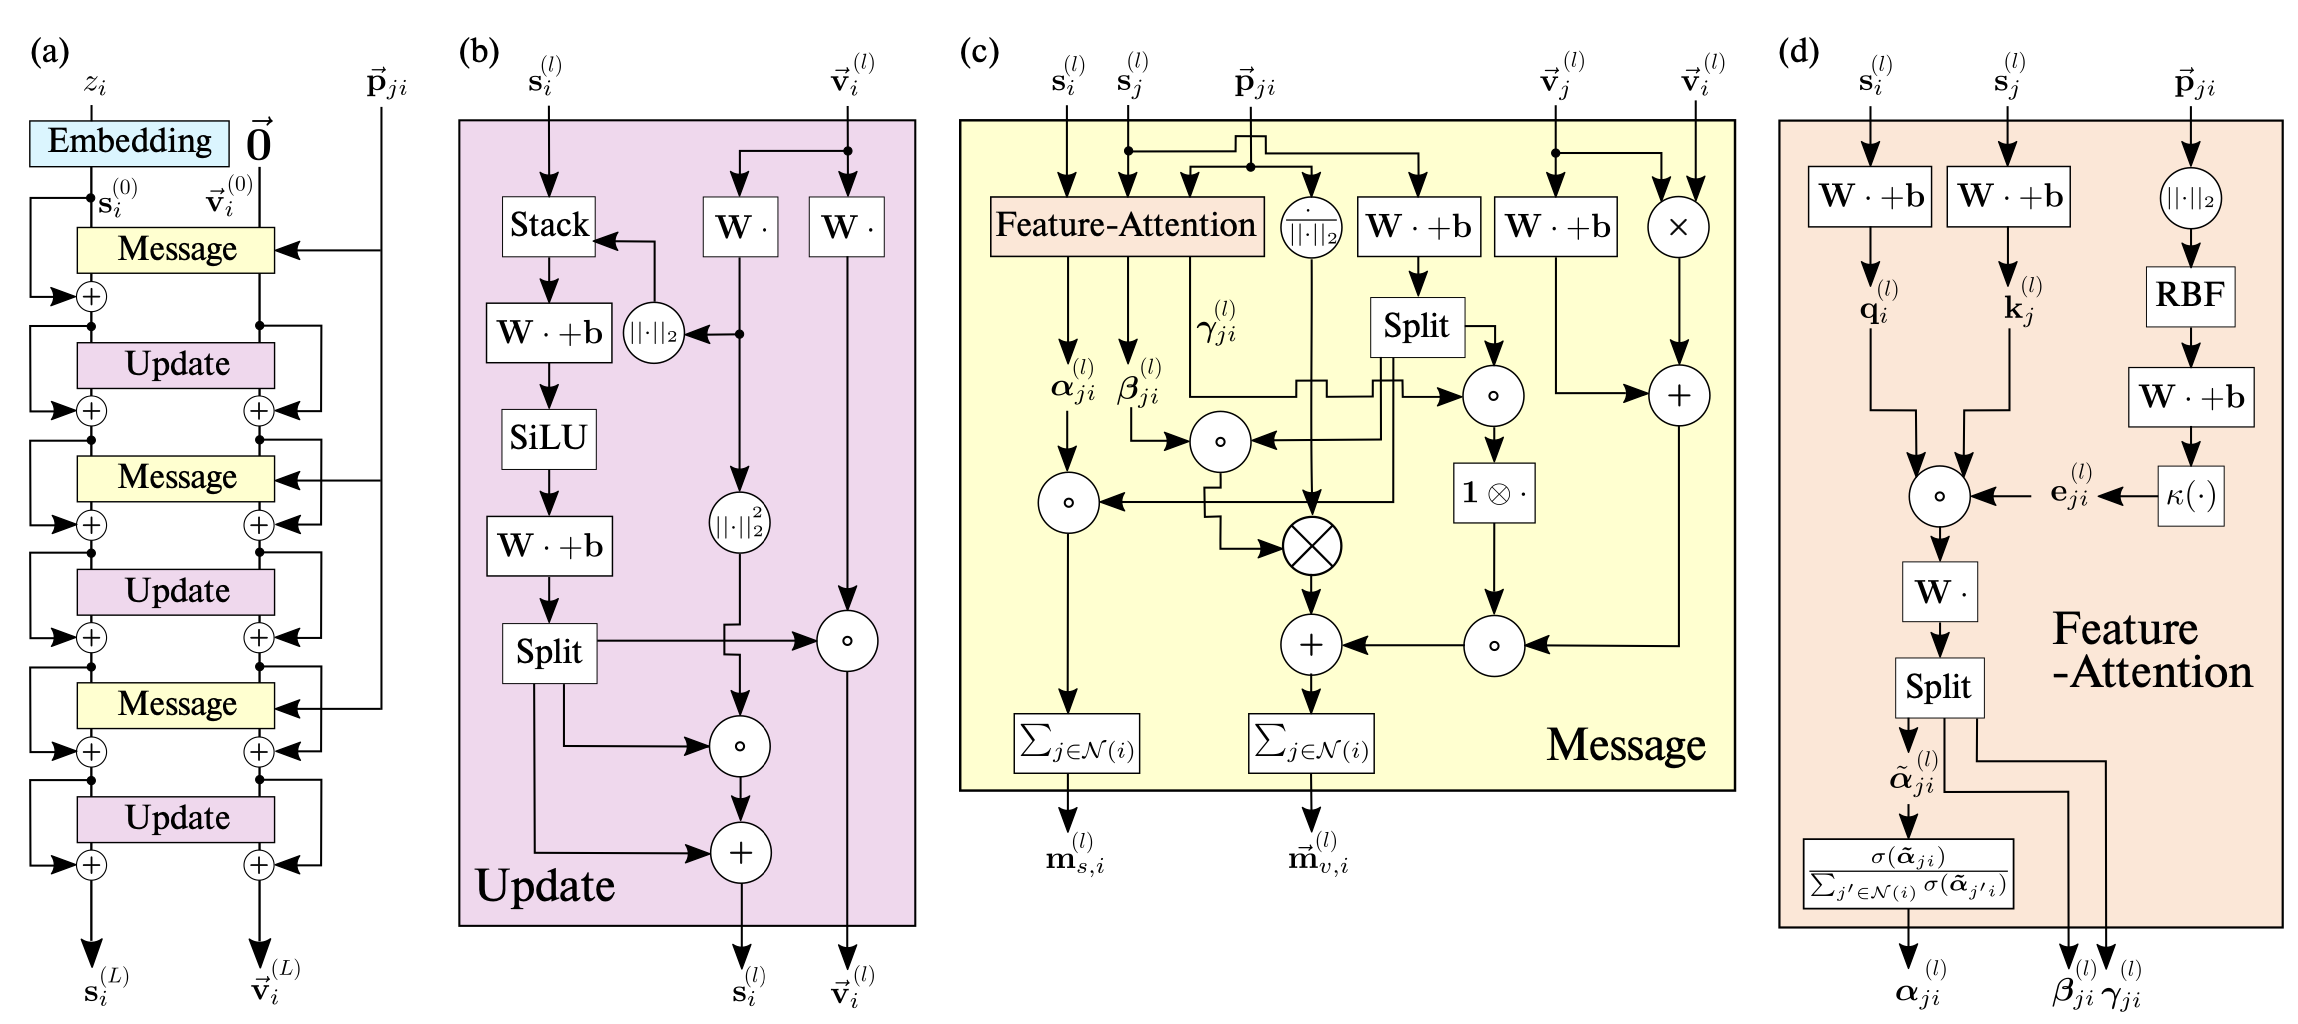
\includegraphics[width=\textwidth]{masters-report/figures/eqgat_diagram.png}
    \caption{(a) The overall message-passing architecture of the EQGAT. (b) The \textit{update} step, allowing information flow from the vector features to the scalar features. (c) The \textit{message construction} step, which creates scalar and vector messages. (d) The \textit{feature-attention} module. Image taken from \cite{eqgat}. }
    \label{eqgat}
\end{figure}

\paragraph{Initial features.}
The initial scalar features used in the model are embeddings created from the atom type of each node, while the initial vector features are set to $\vec{\mathbf{0}}$. Note that after one message-passing layer equivariant vector features are created through the cross-product in Equation \ref{position-cross-product}, which combines the positions of each node with the value tensors created from scalar features. 

Additionally, the edge embedding $\mathbf{e}_{ij}$ encodes the distance between node $i$ and node $j$. We embed the interatomic distance $d_{ij} = ||p_{ij}||_2 \in \mathbb{R}$ using the Bessel radial basis function (RBF), formally defined as:
\begin{equation}
    \text{RBF}_k(d_{ji}) = \sqrt{\frac{2}{c}\frac{\sin(\frac{k\pi}{c}d_{ji})}{d_{ji}}}
\end{equation}
for distance cutoff $c$ and $k = 1, \dots, K$. We concatenate $\text{RBF}_k(d_{ji})$ for all $k = 1,\dots,K$ to obtain an initial edge features $\mathbf{e}^{\text{RBF}}_{ij}$. We pass these through a trainable linear layer and obtain:
\begin{equation}
    \Tilde{\mathbf{e}}_{ji} = \mathbf{W}_e\mathbf{e}^{\text{RBF}}_{ij} + \mathbf{b}_e
\end{equation}
To obtain the final edge embedding, we combine $\Tilde{\mathbf{e}}_{ji}$ with a cosine-cutoff function. The final edge embedding becomes:
\begin{equation}
    \mathbf{e}_{ji} = \frac{1}{2}\Big(\cos (\frac{\pi d_{ji}}{c}) + 1\Big)\cdot \mathbbm{1}[d_{ji}\leq c]\cdot \Tilde{\mathbf{e}}_{ji}
\end{equation}

\subsection{Training hyperparameters}
\label{training-details}
I train two equivariant GNN models on the RES task using the ATOM3D RES dataset \cite{atom-3d}. Both models are trained using one NVIDIA A100 GPU provided by the University's HPC Cluster.  Table \ref{hyperparameters} summarises the hyperparameter configuration of both of my models. Since \citet{eqgat2} do not report the configuration used for training the EQGAT model on the RES task, I instead use the one proposed in the GVP paper for both models. Due to computational constraints, I was unable to perform hyperparameter validation, but I achieve a new state-of-the-art performance on the GVP model, as discussed in Section \ref{sec:res-task}.

\begin{table}[!h]
\centering
\caption{Model architectures and training configuration.}
\vskip 0.15in
\label{hyperparameters}
\begin{tabular}{@{}llll@{}}
\toprule
Hyperparameter                  & \multicolumn{1}{l|}{Value}     & Hyperparameter     & Value     \\ \midrule
Message-passing layers          & \multicolumn{1}{l|}{5}         & Learning rate      & $10^{-4}$ \\
Node features (scalar, vector)  & \multicolumn{1}{l|}{(100, 16)} & Patience scheduler & 10        \\
RBFs                            & \multicolumn{1}{l|}{32}        & Decay rate         & 0.75      \\
RBF cutoff                      & \multicolumn{1}{l|}{4.5 \AA}   & Dropout            & 0.1       \\
EQGAT RBF function              & \multicolumn{1}{l|}{Bessel}    & Batch size         & 64        \\
GVP RBF function                & \multicolumn{1}{l|}{Gaussian}  & Epochs             & 40        \\ \midrule
EQAT total learnable parameters & 469 K                          &                    &           \\
GVP total learnable parameters  & 386 K                          &                    &           \\ \bottomrule
\end{tabular}
\end{table}

\section{Mutation generation}
\label{sec:mutation-generation}
This section describes the strategy used to generate mutations using the two trained GNN models described in Sections \ref{the-gvp-math} and \ref{eqgat-math}. These models are trained to predict the most likely amino acid given a local atomic environment. Based on these capabilities, I repurpose them to the task of mutation generation by masking out each amino acid in a structure \textit{in turn} and passing the masked structure through the model. I then use the scores $l \in \mathbb{R}^{20}$ defined in Equation \ref{logit-scores} to rank the most likely amino acids for each position. Figure \ref{mutation-generation} illustrates this approach visually. 

\begin{figure}[!h]
    \centering
    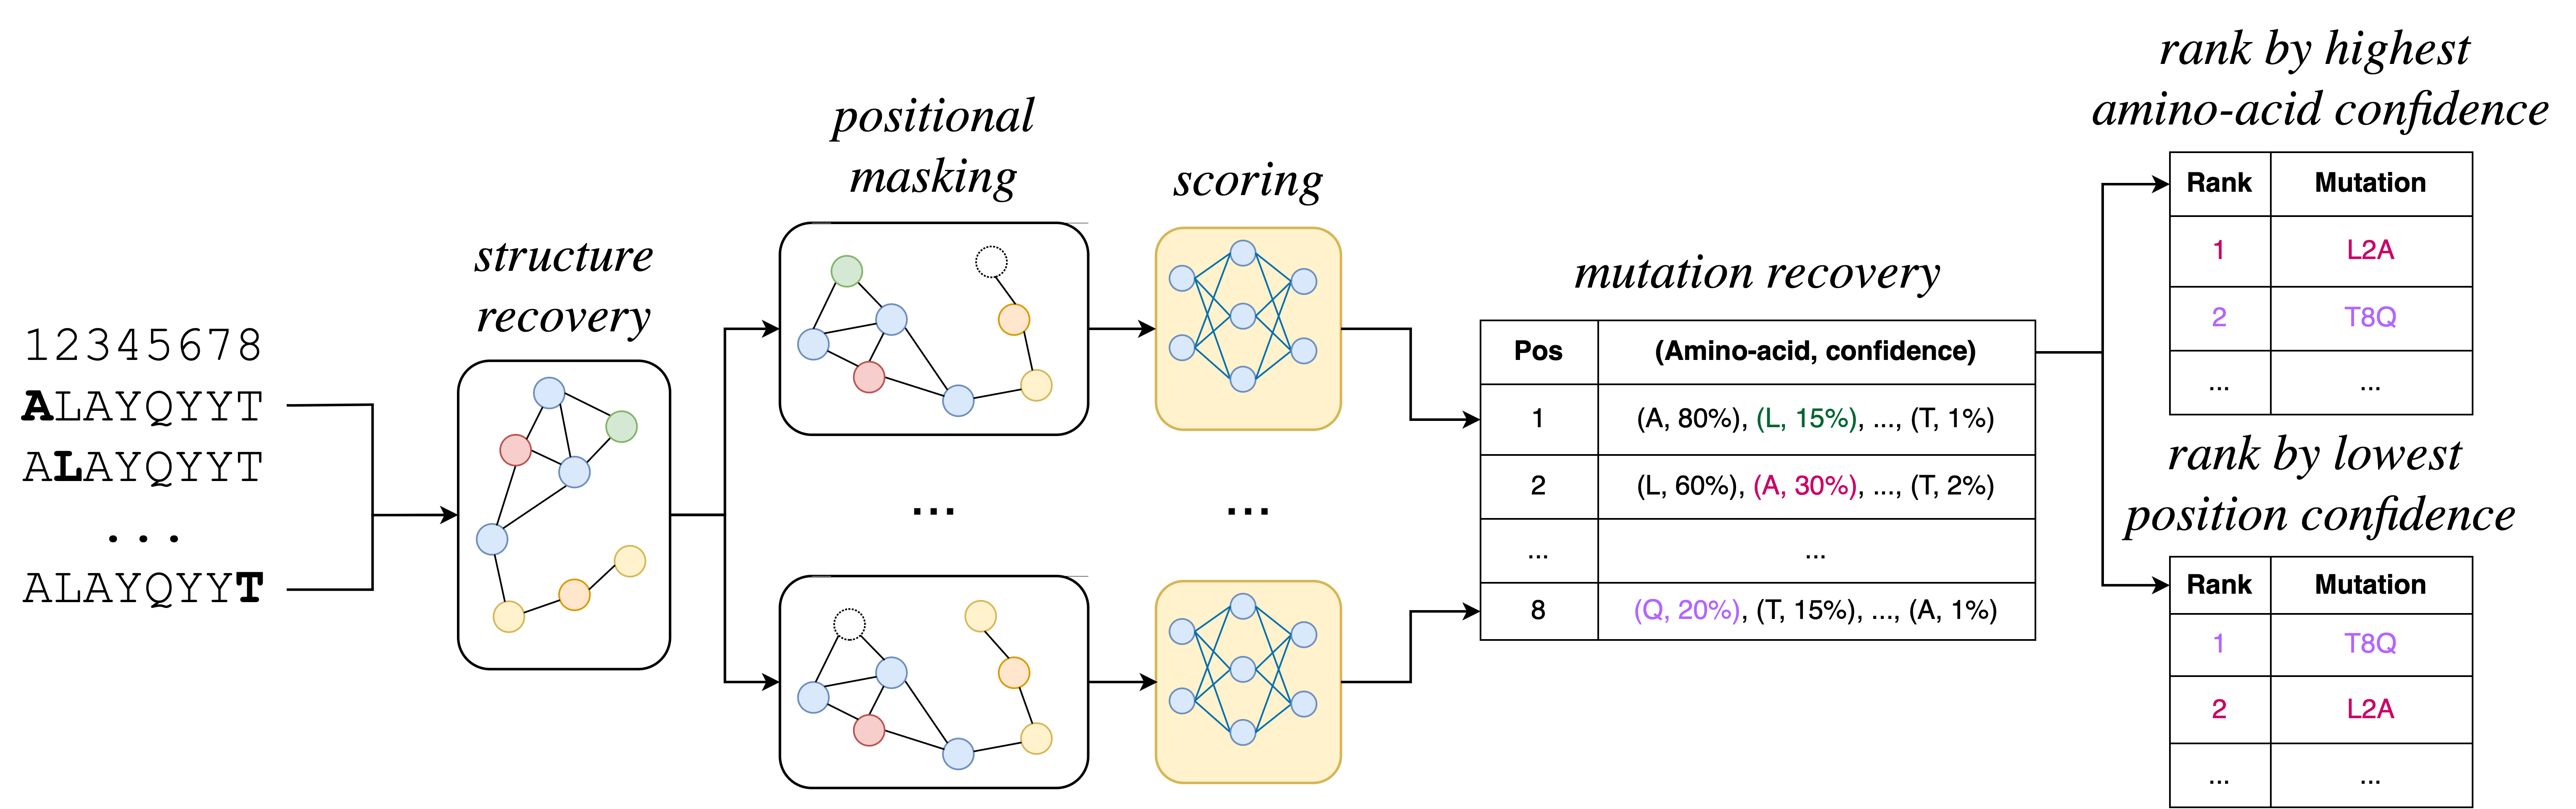
\includegraphics[width=\textwidth]{masters-report/figures/mutation_generation_final.png}
    \caption{Pipeline of phase 2.}
    \label{mutation-generation}
\end{figure}


\subsection{Structure recovery}
\label{sec:structure-recovery}

The ProteinGym substitutions dataset \cite{tranception} contains 87 wildtype sequences. For each of these sequences, a number of experimentally tested mutations are scored according to their \textit{fitness}. While the dataset also includes the fitness of sequences that have been mutated at multiple positions, the scope of this project is limited to \textit{single-point} mutations. 

\paragraph{Monomers and oligomers.} 
As explained in Section \ref{sec:biological-background}, some proteins are part of assemblies. 
When inducing a mutation into a protein that is part of a protein assembly, it must be replicated across all identical chains in the complex. Due to this constraint, I reduce the scope of this project to only deal with sequences whose structures are either \textit{monomers} or \textit{homo-oligomers}. 

The ProteinGym dataset does not provide a mapping between sequences and structures, so the first part of the pipeline illustrated in Figure \ref{mutation-generation} involves the recovery of structures from the Protein Data Bank \cite{rcsb_pdb}. I query the PDB through their programmatic API\footnote{\url{https://search.rcsb.org/index.html\#search-api}} for the biological assembly associated with a sequence. When multiple assemblies are available for the same sequence, I choose the first one returned by the query. 

These assemblies are determined experimentally using X–ray crystallography.\footnote{X-ray crystallography is a method that involves exposing a crystallised sample of a molecule to X-rays in order to determine the positions of individual atoms.} Some experimental assemblies have two challenges. Firstly, the molecule may be bound to a ligand,\footnote{A ligand is usually a smaller molecule that is attached to the main protein and helps it stabilise.} so X-ray crystallography will reveal both the positions of the atoms in the main protein and the atoms in the ligand. To solve this, I apply a post-processing step that cleans the assembly of any undesired ligands or water molecules; the cleaning code is inspired by an approach taken in the AlphaFold \cite{alphafold} codebase.

Secondly, some proteins contain inherently mobile chains that cannot be crystallised. When this is the case, the biological assembly will have an incomplete structure, so I discard the experimental structure and instead use the AlphaFold structural prediction.

\paragraph{AlphaFold structures.} AlphaFold can only predict the structure of monomers. This means that it cannot be easily used to build up hetero-oligomers, and for homo-oligomeric assemblies it will only predict the monomer from which the complex is formed, as exemplified in Figure \ref{alpha-fold-monomer}. The major drawback of using a monomer instead of the entire biological assembly to generate mutations is that amino acids lying on the outskirts of a molecule may be wrongly flagged as viable for mutations, when in reality they should bind to other copies of themselves. A more thorough analysis of the impact of using AlphaFold structures instead of biological assemblies is discussed in Chapter \ref{results}, where an ablation study compares the performance difference when using predicted monomers instead of the full biological assembly.

\begin{figure}[!h]
\centering
    \subfigure[The 6EZM molecule, commonly known as Baker's Yeast. It is formed of 24 copies of the same monomer.]{
        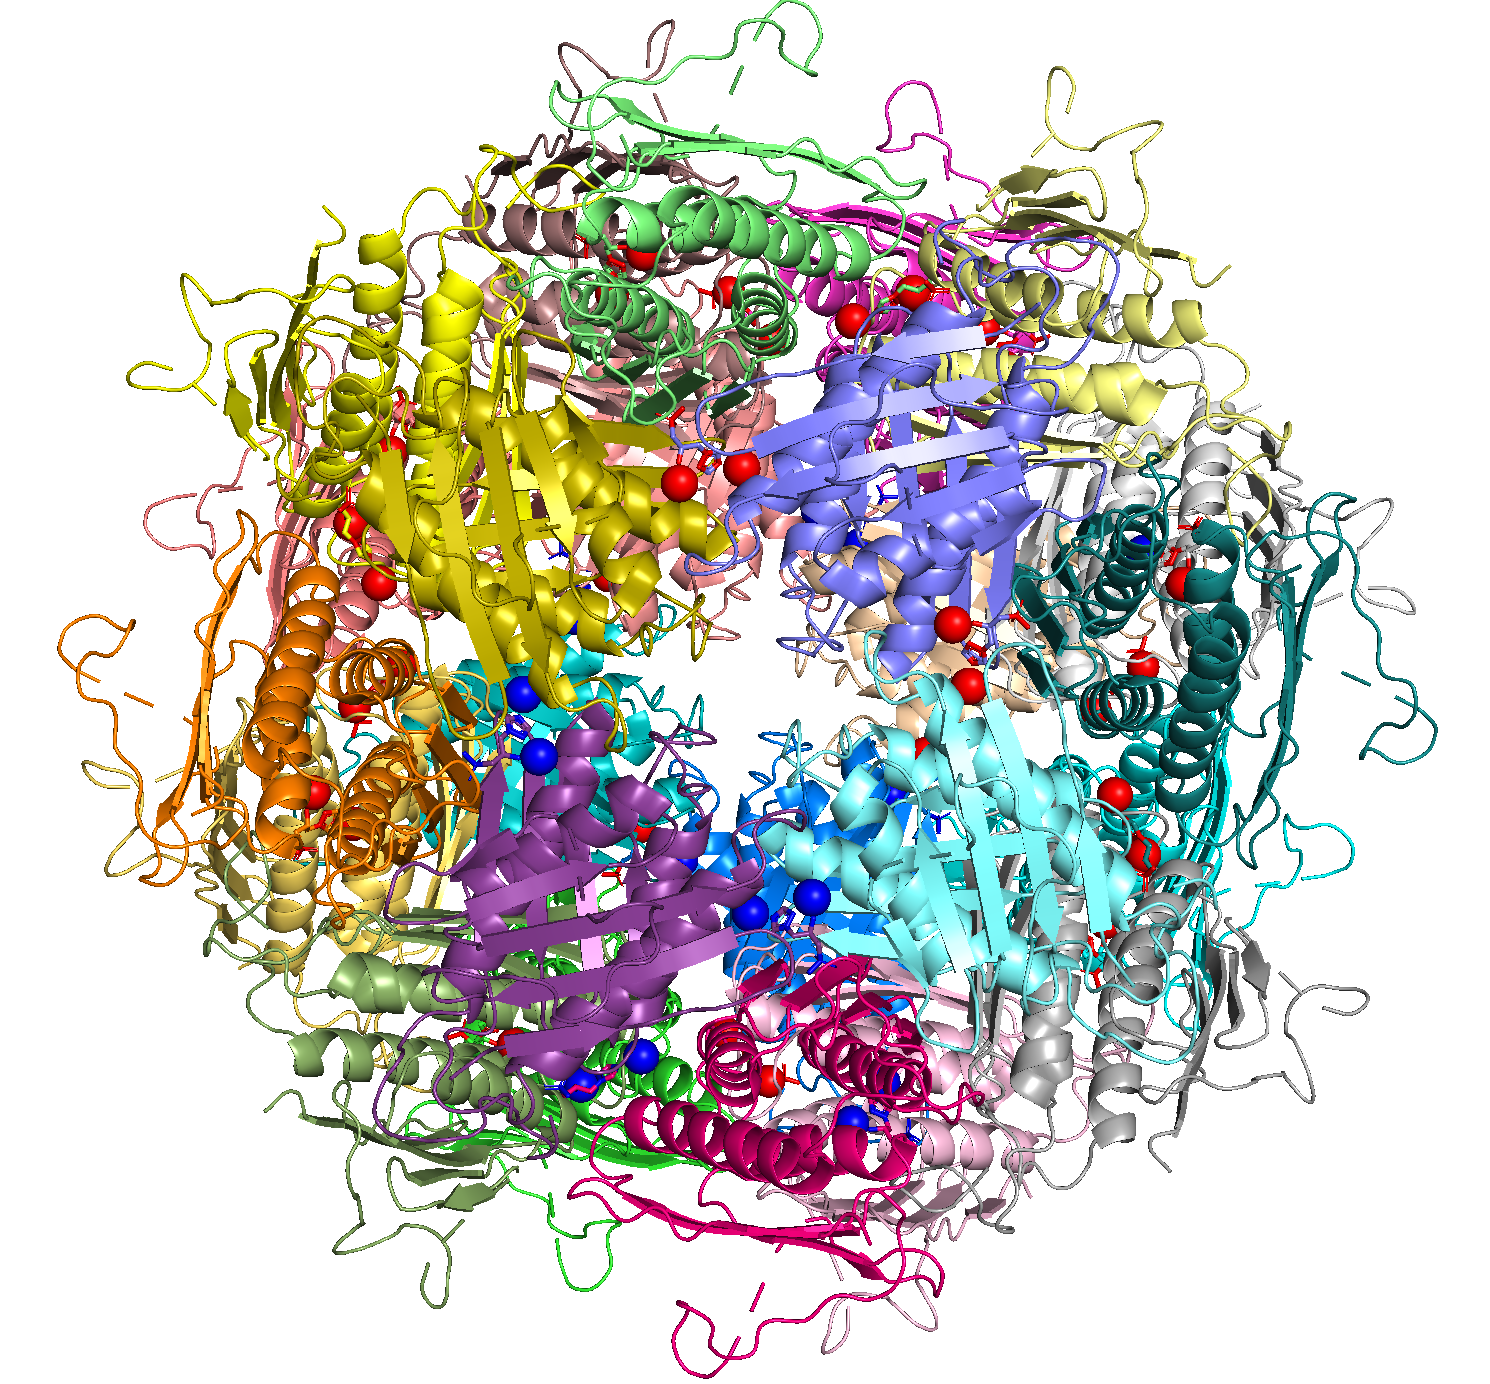
\includegraphics[scale=0.20]{masters-report/figures/6ezm-yeast.png}
        \label{monomer}
    }
    \hspace{0.2in}
    \subfigure[The monomer predicted by AlphaFold for the 6EZM molecule.]{
        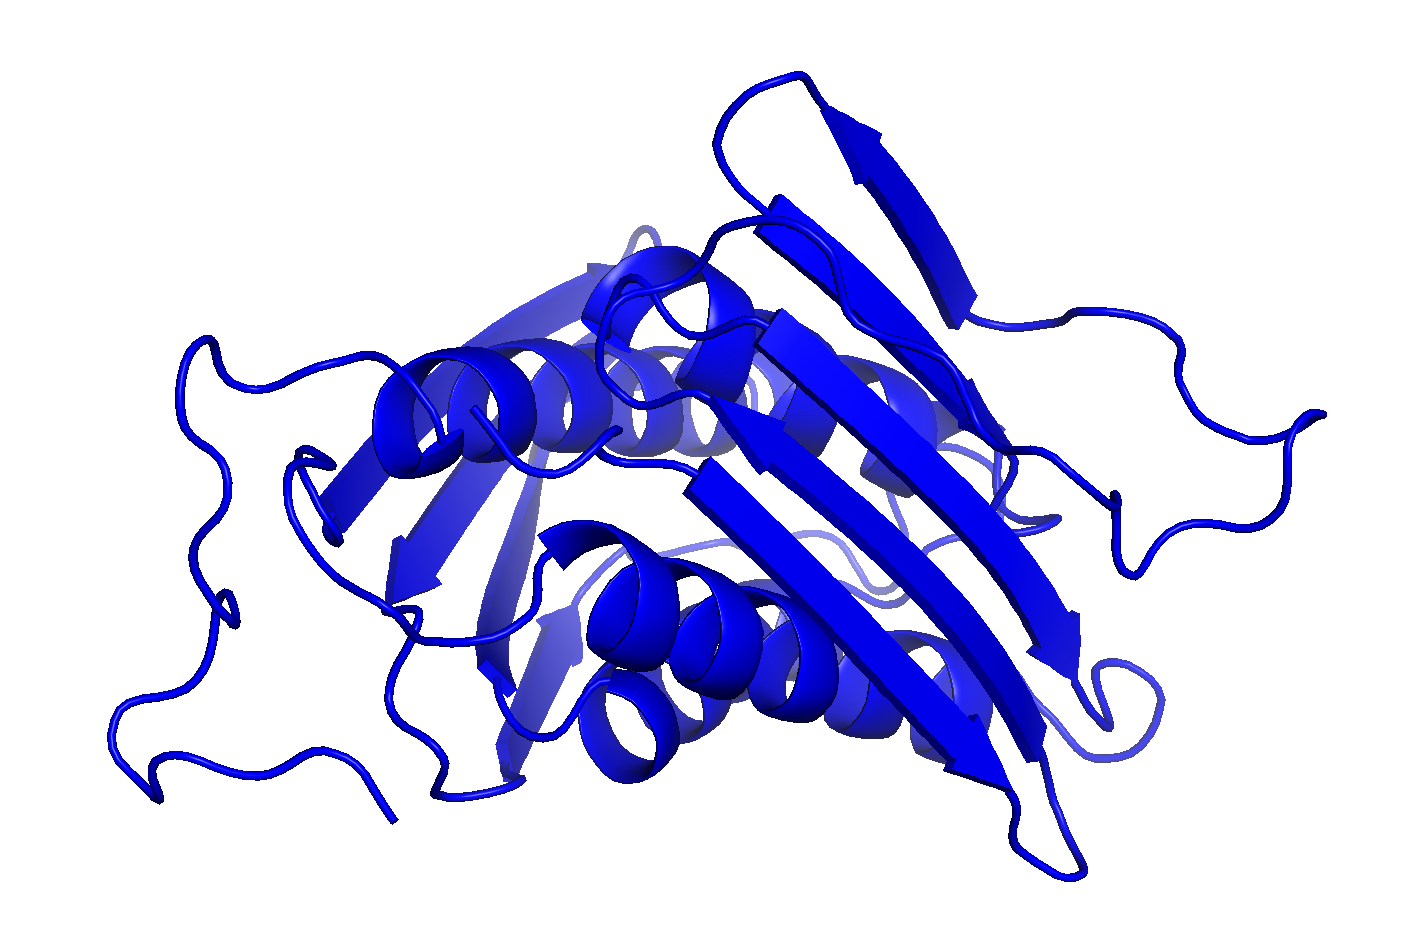
\includegraphics[scale=0.20]{masters-report/figures/alpha-fold-pred.png}
    }
    \caption{Example of (a) a mono 24-mer and  (b) the AlphaFold prediction for the sequence of the mono 24-mer.}
    \label{alpha-fold-monomer}
\end{figure}

The overall structure processing pipeline is presented in Figure \ref{filtering-steps}, which highlights all the points during the post-processing of structures where a design decision is made. 
\begin{figure}[!h]
    \centering
    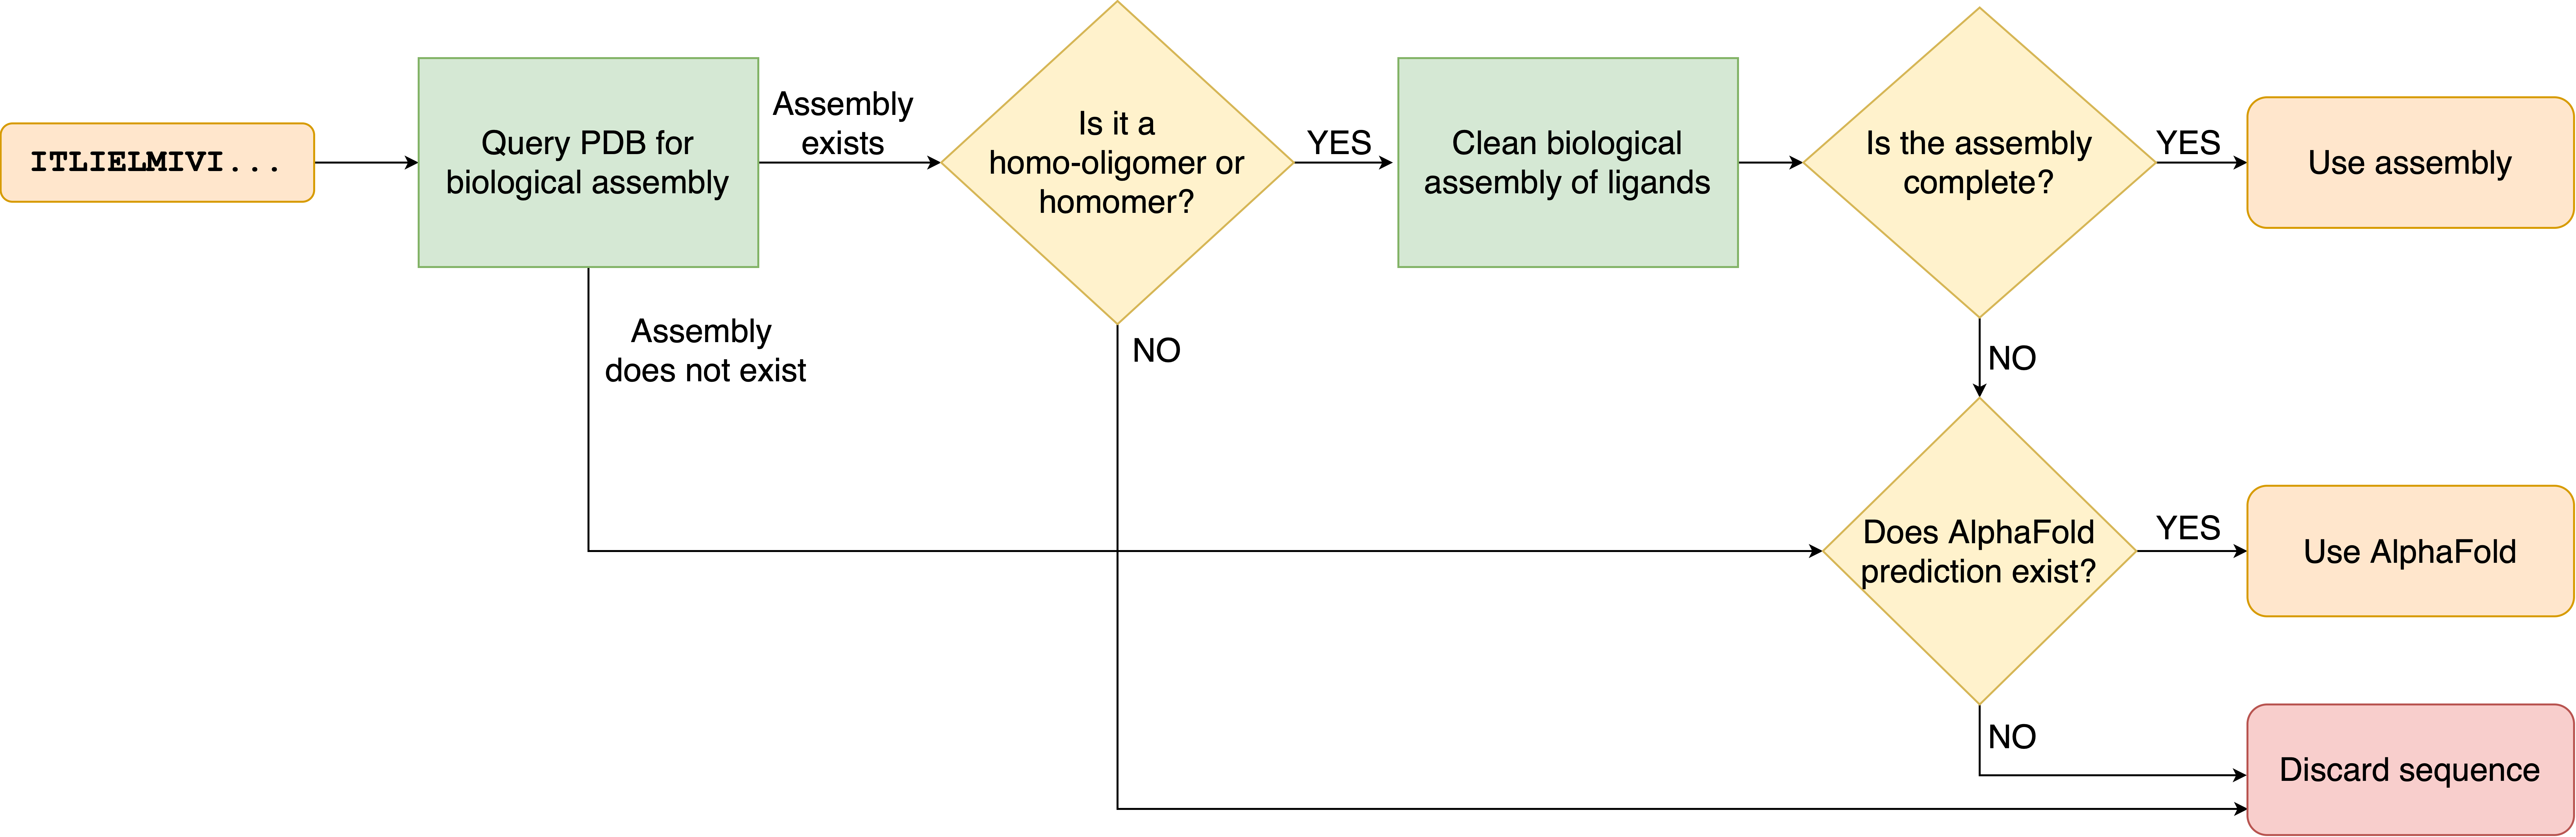
\includegraphics[width=\textwidth]{masters-report/figures/data-process.png}
    \caption{The structure processing pipeline.}
    \label{filtering-steps}
\end{figure}

\subsection{Positional masking}
\label{positional-masking}
The main idea behind the mutation generation strategy is that for every sequence for which I have obtained a clean structure according to the filtering pipeline presented in Figure \ref{filtering-steps} I follow the steps below to determine all possible single-point amino acid mutations in the sequence:
\begin{enumerate}
    \item Firstly, I mask the amino acid residue present at a target position in the structure; 
    \item Secondly, I pass the masked structure through the GNN model; 
    \item Thirdly, I recover the score corresponding to the probability of each of the 20 naturally-occurring amino acids to be in the masked position. 
\end{enumerate}
I repeat this process for all positions in the sequence. 
Intuitively, a higher probability (i.e., model confidence) for a \textit{residue} indicates that the model believes it would be a good match for that position; conversely, an overall lower confidence at a target \textit{position} indicates the position is amenable to mutations.

\subsection{Mutation ranking}
Once I have the scores associated with each of amino acid mutation for every position in a sequence, I propose two strategies for ranking these mutations: global and positional. Formally, given a wildtype sequence $x_1x_2\dots x_n$ of length $n$ with $x_i \in \mathcal{A} = \{1,2,\dots,20\}$ representing the index of amino acid $i$, associated to a atomic graph $\mathcal{G} = (\mathcal{V}, \mathcal{E})$, the process described in \ref{positional-masking} builds a scoring function of the positions  $S:\{1,2,\dots,n\}\times\mathcal{A}\rightarrow \mathbb{R}$ that I define by extending the formalism in Equation \ref{full-formalism}:
\begin{equation}
    S(i, a) = [f_{\gamma}^{g(i)}(\mathbf{H}, \mathbf{E})]_a
\label{scoring-function}
\end{equation}
Where $g:\{1,2,\dots,n\}\rightarrow\{1,2,\dots,|\mathcal{V}|\}$ is a mapping function from positions to the index of the node representing the central $\text{C}_{\alpha}$ of the residue present at said position. 

Equation \ref{scoring-function} essentially represents the score of amino acid $a$ for target position $i$, associated with node $g(i)$ in the atomic graph. Note that the true amino acid at the same position is denoted by $x_i$. 
We are now ready to formally define the two ranking strategies. 

\paragraph{Global ranking.} The first approach to ranking the scores of our mutations is to sort them in descending order of their scores, regardless of the position they occupy. If we denote the single-point mutation to amino acid $a$ at position $i$ by $\mathbf{m}_{i}^a$, then $\forall i,j\text{ and }\forall a,b\in \mathcal{A} \text{ s.t. } a \neq x_i \text{ and } b \neq x_j$, we say that:
\begin{equation}
    \mathbf{m}_{i}^a\text{ is better than }\mathbf{m}_{j}^b \iff S(i, a) > S(j, b)
\label{global-ranking}
\end{equation}

\paragraph{Positional ranking.} The second approach follows when I prioritise the positions I want to mutate instead of the amino acids I mutate to. Instead of quantifying mutations by their global score compared to all other mutations, I rank mutations by the confidence of the model in predicting the wildtype residue at each position. Intuitively, if the model confidence in the wildtype residue $x_i$ at position $i$ is low, this is an indication that the position itself may be prone accept mutations. Formally, this can be quantified as:
\begin{equation}
\begin{aligned}
&\mathbf{m}_{i}^a\text{ is better than }\mathbf{m}_{j}^b \\ 
\iff &\Big(S(i, x_i) < S(j, x_j)\Big) \lor \Big(S(i, x_i) = S(j, x_j) \land S(i, a) > S(j, b)\Big)
\end{aligned}
\label{positional-ranking}
\end{equation}
Equation \ref{positional-ranking} ranks mutations first by their positions; that is, the less confident the model is in a wildtype residue at a certain position, the higher any mutation on that position will rank. In the case of ties (when comparing mutations to different amino acids at the same position), I compare the actual mutation score. I then keep only \textit{the top 3} proposed mutations for each position. 

\section{Protein fitness prediction}
\label{protein-fitness-prediction}
As a second extension to the original scope of the project, I propose a straightforward fitness prediction model that can learn from an already existing dataset of single-point mutations to predict the fitness of a sequences. Following an approach similar to the one used for mutation generation in Section \ref{sec:mutation-generation}, I obtain the scores of all single-point amino acid mutations for every position in every wildtype sequence part of the ProteinGym substitutions dataset \cite{tranception}. I use these scores to augment a baseline regression model to perform protein fitness prediction.

% \begin{figure}
%     \centering
%     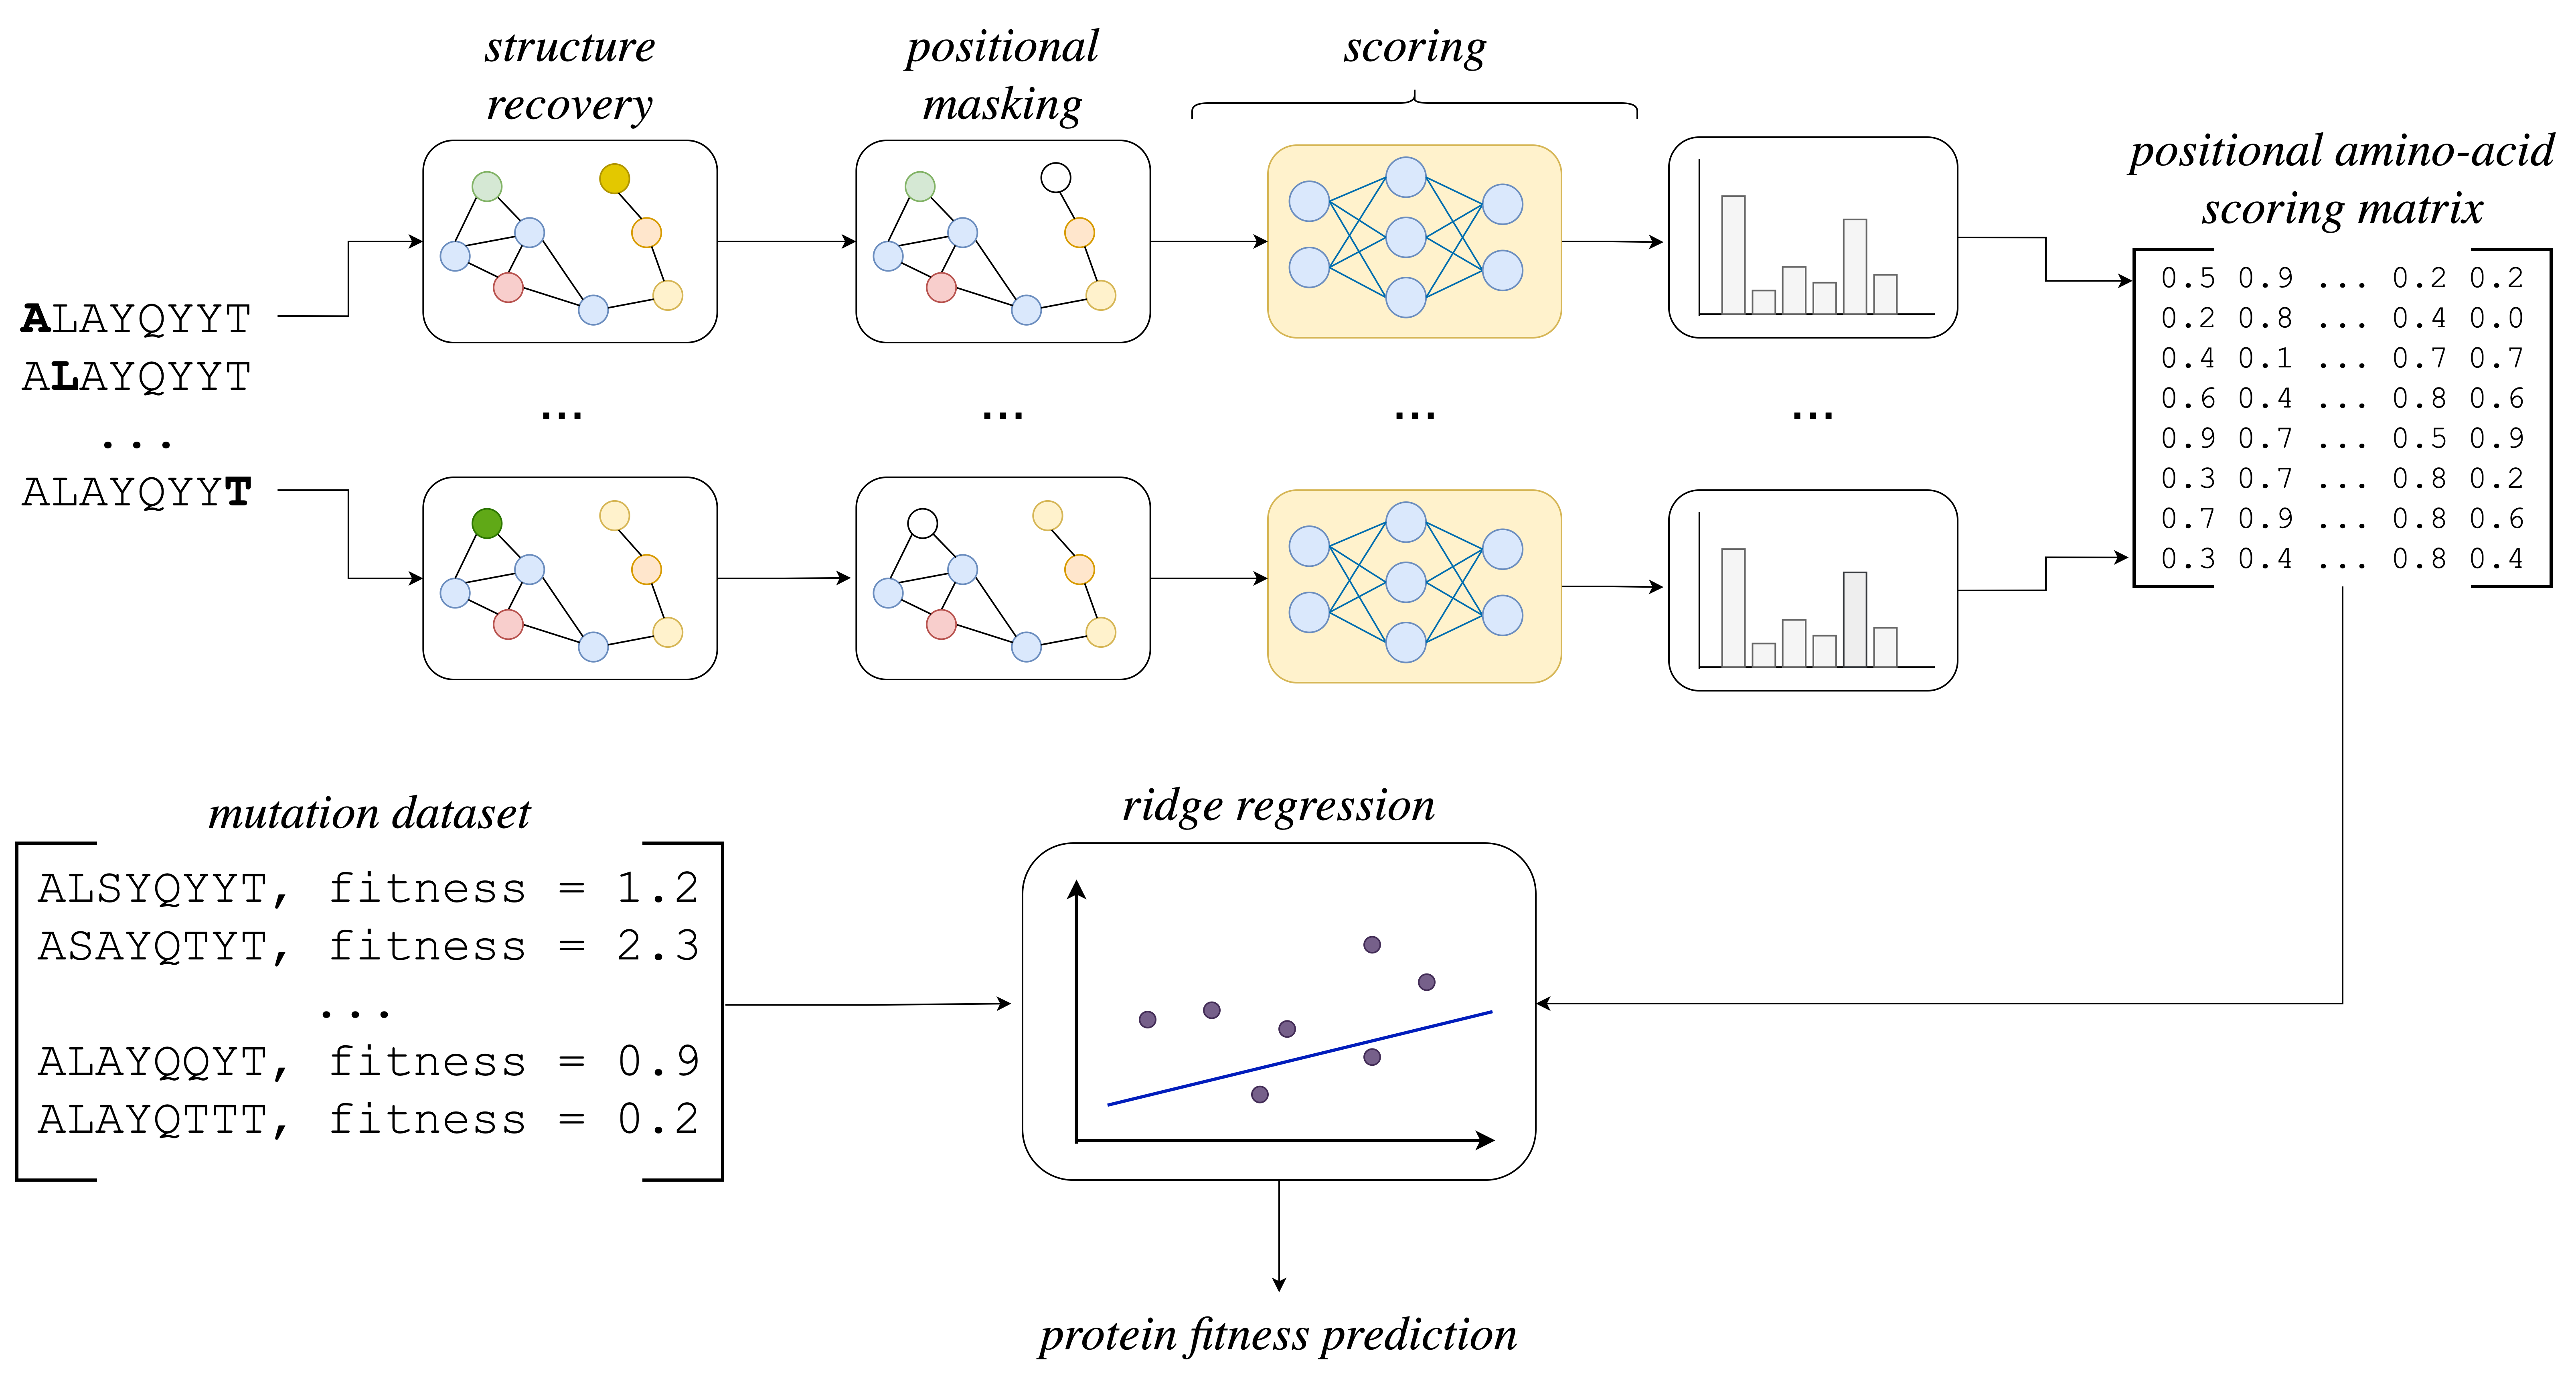
\includegraphics[width=\textwidth]{masters-report/figures/protein_fitness_prediction.png}
%     \caption{Pipeline of phase 3.}
%     \label{fitness-prediction}
% \end{figure}

\subsection{Baseline model} 
I start off with a simple ridge regression model that uses a similar approach to the one proposed by \citet{chloe-hsu}. Formally, for a mutated sequence $s_i = a_1a_2\dots a_n$, we consider its features for the regression to be:
\begin{equation}
    \mathbf{x}_i = [~\text{embed}(a_1) ~||~ \text{embed}(a_2) ~||~ \dots ~||~\text{embed}(a_n)~] ~\in~\mathbb{R}^{n \times d} 
\label{baseline-regression}
\end{equation}
wherd $d\in\mathbb{N}$ is the dimension of the encoding function $\text{embed}:\mathcal{A}\rightarrow \mathbb{R}^d$. The value to predict, $y_i$, represents the fitness of the sequence.

I evaluate two types of encodings in this project:
\begin{enumerate}
    \item The \textbf{one-hot} encoding;
    \item The \textbf{AAIndex} embeddings. The AAIndex database \cite{aa-index} is a database of numeric indicators that represent a wide range of physicochemical and biochemical characteristics of amino acids. I create embeddings from these indices by parsing all known characteristics and performing principle component analysis on them to generate 19-dimensional feature vectors. 
\end{enumerate}

\subsection{Augmented models} 
I augment these simple regression models by adding the score of the single-point mutation present in the sequence $s_i$ to the feature vector $\mathbf{x}_i$. Formally, if sequence $s_i = a_1a_2\dots a_n$ has single-point mutation $\mathbf{m}_i^a$, then the feature vector becomes:
\begin{equation}
    \mathbf{x}_i' = [~\text{embed}(a_1) ~||~ \text{embed}(a_2) ~||~ \dots ~||~ \text{embed}(a_n) ~||~ {\color{blue} S(i, a)}~] ~\in~\mathbb{R}^{n\times d + 1}
\label{augmented-regression}
\end{equation}
Where $S(i, a)$ is the same scoring function as in Equation \ref{scoring-function}. Note that I regularise $S(i,a)$  differently from the rest of the regression features, since the value scale of the score is different from the value scale of the embeddings. This way of creating feature vectors takes into consideration only single-point mutations, hence I add a single new scalar to the feature vector $\mathbf{x}_i$. 
% When dealing with the wildtype sequence, I concatenate either $1$ or $0$ to the original feature vector $\mathbf{x}_i$, depending on the dataset.

% The regression models defined in Equations \ref{baseline-regression} and \ref{augmented-regression} are trained on each wildtype sequence from the ProteinGym dataset separately. These models provide a quick and easy way of predicting the fitness of new mutations given a number of already existing datapoints, hence performing well in a low-data regime. 
\section{Implementation details}

\subsection{Libraries}
The entire implementation of this project was written in the Python programming language.\footnote{\url{https://www.python.org}} I utilised the PyTorch \cite{paszke2019pytorch} and PyTorch Geometric \cite{pyg} frameworks for deep learning components and graph neural network modules. Training was done using PyTorch Lightning,\footnote{\url{https://lightning.ai/docs/pytorch/stable/}} a lightweight wrapper for PyTorch that abstracts away boilerplate code for ML training. I used WandB\footnote{\url{https://wandb.ai/site/papers}} to monitor training runs and log validation metrics. To train the ridge regression models I made use of the \texttt{scikit-learn} Python library.\footnote{\url{https://scikit-learn.org/stable/}}


For processing biological data, I used the following Python libraries: \texttt{biotite}, \texttt{biopandas}, \texttt{biopython}, and \texttt{atom3d}. The former two were used to read and process \texttt{.pdb} files (the format in which protein structures are kept in the Protein Data Bank \cite{rcsb_pdb}), while the latter two were used for miscellaneous biological constants. All protein visualisations presented in this report are generated with PyMol \cite{pymol}.
\subsection{Starting point}
The starting point of this project made use of code from the following three open-source repositories:
\begin{itemize}
    \item \texttt{drorlab/gvp-pytorch}\footnote{\url{https://github.com/drorlab/gvp-pytorch}}: this repository contains the official implementation of the GVP \cite{gvp1, gvp2} module. My supervisor provided an optimised version of this architecture that I could use for faster training on the RES task. I adapted my supervisor's code to fit into my Pytorch Lightning training framework. 
    \item \texttt{Bayer-Group/eqgat}\footnote{\url{https://github.com/Bayer-Group/eqgat}}: this repository contains the official implementation of the EQGAT \cite{eqgat, eqgat2} architecture. I adapted this code to fit into my Pytorch Lightning training framework. 
    \item \texttt{deepmind/alphafold}\footnote{\url{https://github.com/deepmind/alphafold/blob/a3941673e90b8d1d75c60b16a4b3707ebf7ba527/alphafold/relax/cleanup.py}}: this repository contains the official implementation of the AlphaFold \cite{alphafold} model. From here I adapted code to clean experimental protein structures. 
\end{itemize}
For the evaluation against all sequence-based models, I used results available in the \texttt{OATML-Markslab/Tranception} repository.\footnote{\url{https://github.com/OATML-Markslab/Tranception}}

\chapter{Evaluation}
\label{results}
\section{Pre-training: RES task performance}
\label{sec:res-task}
In the first phase (Section \ref{res-task}), I train two equivariant GNN models on the RES task, using the ATOM3D dataset. The ATOM3D RES \cite{atom-3d} dataset is large, with over 3 million graph samples. As a consequence, the models have taken around a week each to train using one NVIDIA A100 GPU. Due to this constraint, I report the test accuracy resulting from a single training run on each of the two models. 

Table \ref{model-accuracy} summaries the test accuracies of the trained models.
\begin{table}
\caption{Classification accuracies on the ATOM3D RES dataset.}
\label{model-accuracy}
\vskip 0.15in
\begin{center}
\begin{small}
\begin{sc}
\begin{tabular}{@{}lcc@{}}
\toprule
Model & \begin{tabular}[c]{@{}c@{}}Reported test accuracy\end{tabular} & \begin{tabular}[c]{@{}c@{}}My test accuracy\end{tabular} \\ \midrule
EQGAT & 0.540                                                             & 0.524                                                        \\
GVP   & 0.527                                                             & \textbf{0.580}                                               \\ \bottomrule
\end{tabular}
\end{sc}
\end{small}
\end{center}
\vskip -0.1in
\end{table}
I was unable to replicate the test accuracy reported by \citet{eqgat2} on the RES task. One possible reason is a mismatch in the hyperparameter configuration, which the original authors do not report for the RES task. However, due to the computational constraints mentioned above, it was unfeasible to perform further hyperparameter tuning to determine the best setup. 

Surprisingly, I report a much higher accuracy for the GVP architecture than originally stated in \cite{gvp2}. One possible explanation is that \citet{gvp2} train their GVP model on 1 million sampled graphs from the ATOM3D RES dataset, therefore using only a third of the full training dataset. In light of this, I report that the GVP model trained on the full ATOM3D RES dataset achieves a new state-of-the-art performance on the RES task, with an accuracy of \textbf{58\%}. 

\subsection{How good should a model be?}
\label{training-discussion}
Since I use these models as mutation generation engines, one tricky question is when to stop training: that is, when the model predicts an amino acid wrongly, is it because the model made a mistake, \textit{or is it because Nature made a mistake?} In this project, I stop training after 40 epochs due to computational constraints, although the validation curves of both models do not show clear signs of overfitting, as can be seen in Figure \ref{train-plots}.

\begin{figure}[!htb]
    \centering
    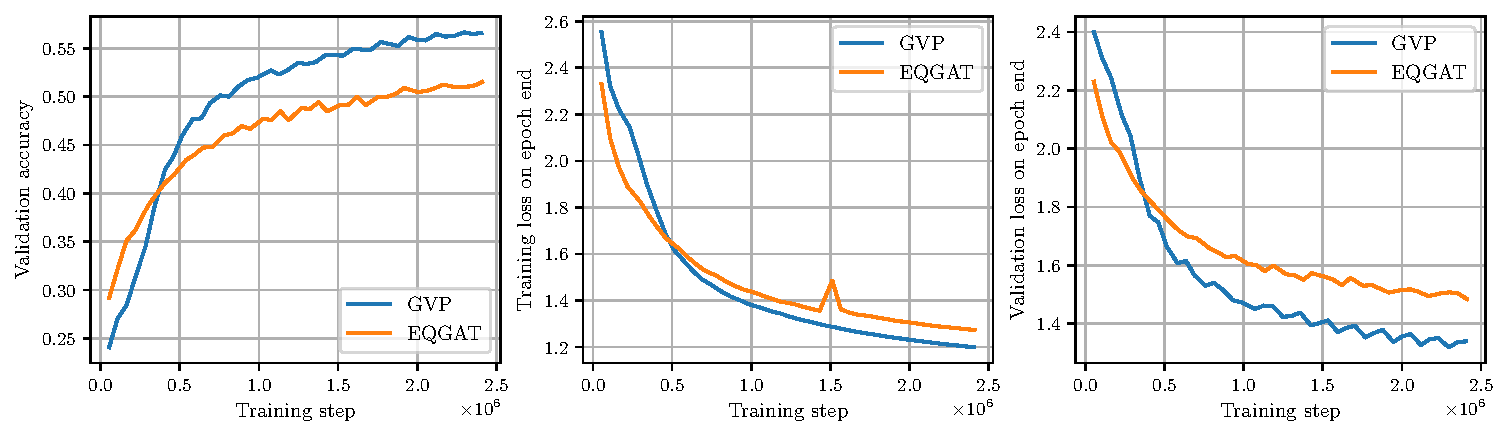
\includegraphics[width=\textwidth]{masters-report/figures/validation_acc.pdf}
    \caption{Accuracy and loss values across 40 epochs.}
    \label{train-plots}
\end{figure}

As it is discussed in Section \ref{mutation-discard}, I perform an ablation study in which I compare the performance of the two ranking techniques when I ignore mutations at positions that the models got wrong. Since the models perform \textit{better} when I discard these mutations, this is an indication that the models themselves are still \textit{undertrained}, thereby having a higher capacity for mutation generation than the one achieved in this project. 

\section{Evaluation metrics}
The main aim of my approach to mutation generation is to find mutations that are better than the wildtype sequence. To quantify how good my models are for predicting promising mutations, I am particularly interested in 3 metrics: Spearman's rank correlation for better than wildtype mutations, the top 10 precision, and the top 10 recall. I briefly present the motivation behind all three metrics below. 

\subsection{Spearman's rank correlation} 
The Spearman rank correlation, also known as Spearman's $\rho$, is a statistical measure that assesses the strength and direction of the monotonic relationship between two variables. It is formally defined as the Pearson correlation coefficient between rank variables. For a sample of size $n$, the $n$ raw scores $X_i$ and $Y_i$ are converted to ranks $R(X_i)$ and $R(Y_i)$. Then, the coefficient $r_s$ is computed as:
\begin{equation}
    r_s = \frac{\text{cov}(R(X), R(Y))}{\sigma_{R(X)}\sigma_{R(Y)}}
\end{equation}
where $\sigma_{R(X)}$ and $\sigma_{R(Y)}$ are the standard deviations of the rank variables. 

I am interested in quantifying the performance of my approach in predicting single-point mutations that are better than the wildtype sequence. Hence, one of the metrics I am interested in is the Spearman rank correlation for better than wildtype mutations only. That is, I discard predicted mutations for which the true fitness (found in the ProteinGym dataset) is lower than the fitness of the wildtype sequence.

In contrast to this approach, \citet{tranception}, who propose Tranception, only report the \textit{average} Spearman rank correlation between their model's prediction and the true fitness. To produce a fair comparison, I report both the average Spearman and the better than wildtype Spearman for the EQGAT and GVP, as well as for representatives of the sequence-based approaches: Tranception \cite{tranception}, ESM-1v \cite{meier2021language}, and the MSA Transformer \cite{Rao2020}.

\subsection{Precision and recall} 

Precision and recall are two metrics used in evaluating the performance of classification models, particularly in the field of information retrieval and machine learning. They are commonly used together to provide a comprehensive assessment of a model's effectiveness.

% Precision measures the proportion of correctly predicted positive instances out of all instances predicted as positive. It focuses on the reliability of positive predictions, hence a high precision means that the model has a low rate of false positives. The formula for precision is:
% \begin{equation}
% \text{Precision} = \frac{\text{True Positives}}{\text{(True Positives + False Positives)}}
% \end{equation}
% Recall can be considered complimentary to precision, as it measures the proportion of correctly predicted positive instances out of all actual positive instances. It focuses on the overall ability of the model to identify positive instances. The formula for recall is:
% \begin{equation}
% \text{Recall} = \frac{\text{True Positives}}{\text{(True Positives + False Negatives)}}
% \end{equation}
% As mentioned before, we are interested in the models' ability to predict promising mutations. We therefore treat mutations as positives if they are better than the wildtype and negatives otherwise. 

\paragraph{Top-k precision and recall.}
Top-k precision measures the proportion of correctly predicted positive instances among the top-k predictions made by the model.
The formula for top-k precision is:
\begin{equation}
\text{Top-k Precision} = \frac{\text{(Number of true positives within top-k)}}{k}
\end{equation}
Top-k recall measures the proportion of correctly predicted positive instances among all the relevant instances, considering only the top-k predictions made by the model. The formula is:
\begin{equation}
    \text{Top-k Recall} = \frac{\text{(Number of true positives within top-k)}}{\text{(Total number of better than wildtype mutations)}}
\end{equation}

Note that the recall is calculated relative to the number of mutations predicted by each model, rather that relative to the total number of mutations in each DMS assay from ProteinGym. 

In this project I report the top-10 precision and the top-10 recall, because my aim is to build an easy to use tool for researchers to accelerate their discovery process, and having a list of the top 10 mutations that are considered promising is a straightforward way of aiding the exploratory process. 

\section{Mutation generation}
\label{sec:mutation-generation-results}
For mutation ranking, I use the DMS assays of 49 sequences out of the total of 87 that exist in the ProteinGym substitutions dataset. These 49 sequences are either monomers or homo-oligomers for which I could find either a complete experimental structure or an AlphaFold predicted structure, as discussed in Section \ref{sec:structure-recovery}.

Before presenting the results to mutation ranking, it is important to note that my approach generates mutations, rather than predicting the fitness of already existing ones. This means some of the proposed mutations will not exist in the ProteinGym dataset; when this is the case, I discard them, as there is no other way of evaluating their fitness other than in the wet lab, and this would be beyond the scope of this project.

Additionally, when ranking the mutations generated by the EQGAT and the GVP models, I choose to \textit{discard} mutations proposed at positions where the models failed to predict the true wildtype residue. Formally, given a sequence $x_1x_2\dots x_n$, I discard all mutations $\mathbf{m}_i^a$ proposed for position $i$ if there exists an amino acid $b$ such that $S(i, b) > S(i, x_i)$. A broader discussion on the motivation behind this design choice can be found in Section \ref{mutation-discard}. 

Table \ref{mutation-generation} summaries the performance of my approach to mutation ranking. As we can see, although the MSA Transformer \cite{tranception} achieves the highest overall Spearman rank correlation, it performs poorly when only considering mutations that are better than the wildtype. 
A per-dataset breakdown of the performance of EQGAT, GVP, and Tranception can be found in Appendix \ref{appendix:per-dataset-breakdown}.

\begin{table*}[!htb]
\caption{\raggedright{Ranking performance of the models across 49 DMS assays. Numbers in \textbf{bold} represent the highest score per column, while numbers with an \underline{underline} represent the second highest score per column. We note that two equivariant GNNs have the highest rank correlation for better than wildtype mutations.}}
\label{generation-results}
% \vskip 0.15in
\begin{center}
\begin{small}
\begin{sc}
\begin{tabular}{@{}ccccccc@{}}
\toprule
\multirow{2}{*}{Model} & \multirow{2}{*}{\begin{tabular}[c]{@{}c@{}}Ranking \\ strategy\end{tabular}} & \multirow{2}{*}{\begin{tabular}[c]{@{}c@{}}Top 10\\ precision\end{tabular}} & \multirow{2}{*}{\begin{tabular}[c]{@{}c@{}}Top 10\\ recall\end{tabular}} & \multicolumn{3}{c}{Spearman's rank correlation}                                                                                       \\ \cmidrule(l){5-7} 
                       &                                                                              &                                                                             &                                                                          & All        & \begin{tabular}[c]{@{}c@{}}Worse than \\ WT\end{tabular} & \begin{tabular}[c]{@{}c@{}}Better than \\ WT\end{tabular} \\ \midrule
EQGAT                  & Positional                                                                   & 0.486                                                                       & \underline{0.187}                                                              & 0.223          & 0.128                                                    & 0.118                                                     \\
EQGAT                  & Global                                                                       & 0.491                                                                       & 0.072                                                                    & 0.262          & 0.154                                                    & \underline{0.157}                                               \\
GVP                    & Positional                                                                   & 0.462                                                                       & \textbf{0.419}                                                           & 0.106          & -0.009                                                   & \textbf{0.276}                                            \\
GVP                    & Global                                                                       & 0.426                                                                       & 0.100                                                                    & 0.202          & 0.128                                                    & -0.011                                                    \\ \midrule
Tranception            &                                                                              & \underline{0.619}                                                                 & 0.012                                                                    & \underline{0.429}    & \underline{0.299}                                              & 0.143                                                     \\
ESM-v1                 &                                                                              & 0.618                                                                       & 0.018                                                                    & 0.407          & 0.288                                                    & 0.135                                                     \\
MSA Trans.        &                                                                              & \textbf{0.638}                                                              & 0.018                                                                    & \textbf{0.434} & \textbf{0.327}                                           & 0.135                                                     \\ \bottomrule
\end{tabular}
\end{sc}
\end{small}
\end{center}
\vskip -0.1in
\end{table*}



\paragraph{The ranking approach.}
I note that the GVP model achieves the best ``better than WT'' Spearman rank correlation to the ProteinGym fitness values. This performance seems to be highly dependent on the type of ranking used, as the correlation drops from $\mathbf{0.27}$ to virtually $\mathbf{0}$ when switching from positional to global ranking. Additionally, positional ranking keeps only the \textit{top 3} mutations per position, hence this approach would actually generate \textbf{fewer} mutations instead of proposing worse ones. 
% This is also indicated by the high top-10 recall of the same approach, namely $\mathbf{0.41}$, which suggests that, on average, the top 10 mutations proposed by the GVP account for almost half of all the better than wildtype mutations the model generates (and are found in the ProteinGym dataset).

\paragraph{Data efficiency.}
EGNN models require a significantly smaller number of protein structures during training in order to reach a similar ranking correlation coefficient to the sequence-based models for mutations that are better than the wildtype. While these models are typically trained on massive amounts of data (e.g. 350 million sequences in the case of Tranception) my models are trained on fewer than 22k molecules from which local environments are sampled. This, coupled with the fact that these structural models have not reached their capacity (as mentioned Section \ref{training-discussion}), indicates that these EGNN models to be \textit{further fine-tuned} by small research groups for task specific purposes. 

\paragraph{Correlation to sequence-based models.}
As part of my analysis, I also compute the correlation between the better than wildtype predictions made by the EGNN models and Tranception. Per-model and per-dataset statistics can be found in \ref{tranception-correlation}; I note that the highest rank correlation I find is \textbf{0.212}, in the case of the EQGAT model. Since these approaches seem to be weakly correlated, I believe there are improvements to be gained from ensembling both structure- and sequence-based approaches.

Note that in the case of the EQGAT model, changing the ranking strategy does not result in a significant performance drop, indicating that the model identifies both the good positions and the good amino acids to perform mutations, but performs worse overall.

\subsection{Ablation studies}
The development of performant structure-based models for mutation generation involved design decisions that impacted how proteins are processed by my models and whether certain mutations are kept or discarded from the overall ranking. 
For the purposes of aiding future the engineering efforts of designing good structure-based methods, I report a few ablation studies that justify the decisions made for the main evaluation. A summary of the findings suggest the following: 
\begin{itemize}
    \item Discarding positions where the models cannot correctly identify the true wildtype amino acid increases the quality the mutation ranking (Tables \ref{ablation-correct-only-global} and \ref{ablation-correct-only-positional});
    \item Using the AlphaFold structure is \textit{not} detrimental to the generation of better than wildtype mutations (see Appendix \ref{appendix-exp-vs-alphafold}: Tables \ref{ablation-alphafold-global} and \ref{ablation-alphafold-positional});
    \item The EQGAT model works best with the full molecular structure, while the GVP model works best with the local environment (see Appendix \ref{appendix-full-vs-local}: Tables \ref{ablation-local-environment-global} and \ref{ablation-local-environment-positional}).
\end{itemize}

\subsubsection{Discarding wrongly predicted positions}
\label{mutation-discard}
As mentioned at the beginning of Section \ref{sec:mutation-generation-results}, I add an additional filter to my ranking techniques in order to increase the quality of the mutations proposed by the models. More specifically, I discard all mutations at a position that was classified incorrectly by the EGNN. An incorrect classification of a residue may indicate that the models do not have a good understanding of the biophysical properties of the residue's local environment. This is particularly damaging to the generation of meaningful mutations if a models assigns similarly low confidences to all 20 amino acids that are candidate for a position because it resorts to random guessing. 

I provide an ablation study to back up this design choice. Tables \ref{ablation-correct-only-global} and \ref{ablation-correct-only-positional} show how, overall, keeping all mutations generated by any structure-based model decreases its performance. 

\begin{table}[!hbt]
\caption{Model performance when performing \textbf{global} ranking using both wrongly and correctly predicted positions. Statistics averaged across for 49 DMS assays.}
\label{ablation-correct-only-global}
\vskip 0.15in
\begin{center}
\begin{small}
\begin{sc}
\begin{tabular}{@{}ccccc@{}}
\toprule
\multirow{2}{*}{Model} & \multirow{2}{*}{Positions used} & \multicolumn{3}{c}{Spearman's rank correlation}  \\ \cmidrule(l){3-5} 
                       &                                 & Average        & Worse than WT  & Better than WT \\ \midrule
EQGAT                  & all                             & 0.20           & 0.153          & 0.069          \\
EQGAT                  & correct only                    & \textbf{0.262} & \textbf{0.154} & \textbf{0.157} \\ \midrule
GVP                    & all                             & 0.093          & 0.076          & \textbf{0.014} \\
GVP                    & correct only                    & \textbf{0.202} & \textbf{0.128} & -0.011         \\ \midrule
Tranception            &                                 & 0.429          & 0.299          & 0.143          \\ \bottomrule
\end{tabular}
\end{sc}
\end{small}
\end{center}
\vskip -0.1in
\end{table}

\begin{table}[!hbt]
\caption{Model performance when performing \textbf{positional} ranking using both wrongly and correctly predicted positions. Statistics averaged across for 49 DMS assays.}
\label{ablation-correct-only-positional}
\vskip 0.15in
\begin{center}
\begin{small}
\begin{sc}
\begin{tabular}{@{}ccccc@{}}
\toprule
\multirow{2}{*}{Model} & \multirow{2}{*}{Positions used} & \multicolumn{3}{c}{Spearman's rank correlation}             \\ \cmidrule(l){3-5} 
                       &                                 & Average        & Worse than WT & Better than WT \\ \midrule
EQGAT                  & all                             & 0.124          & 0.100               & 0.061                \\
EQGAT                  & correct only                    & \textbf{0.223} & \textbf{0.128}      & \textbf{0.118}       \\ \midrule
GVP                    & all                             & 0.083          & \textbf{0.076}      & -0.018               \\
GVP                    & correct only                    & \textbf{0.106} & -0.009              & \textbf{0.276}       \\ \midrule
Tranception            &                                 & 0.429          & 0.299               & 0.143                \\ \bottomrule
\end{tabular}
\end{sc}
\end{small}
\end{center}
\vskip -0.1in
\end{table}

\paragraph{Analysing undertraining.}
We can get a better idea of the types of information that is learned by the EGNN models by looking at the confusion matrices between the true labels and the predicted labels in the ATOM3D RES test dataset, illustrated in Figure \ref{fig:confusions}. I compare these two matrices to the BLOSUM62 matrix, a scoring matrix commonly used in bioinformatics for sequence alignment; each cell represents the score for substituting one amino acid with another. Higher scores indicate a higher degree of conservation or similarity between the substituted amino acids.

I expect that models with meaningful inferred knowledge about the biophysical properties of amino acids to have a similar confusion matrix to the BLOSUM62 matrix; while some parts of the confusion matrix do resemble BLOSUM62 (e.g., Cystine (C) is not easily confused with any of its neighbouring amino acids), it seems that the models are still undertrained. I do, however, notice that the confusion matrices of the EQGAT and the GVP look similar to each other, indicating that they must be learning the same features from the training dataset.  

\begin{figure}
    \centering
    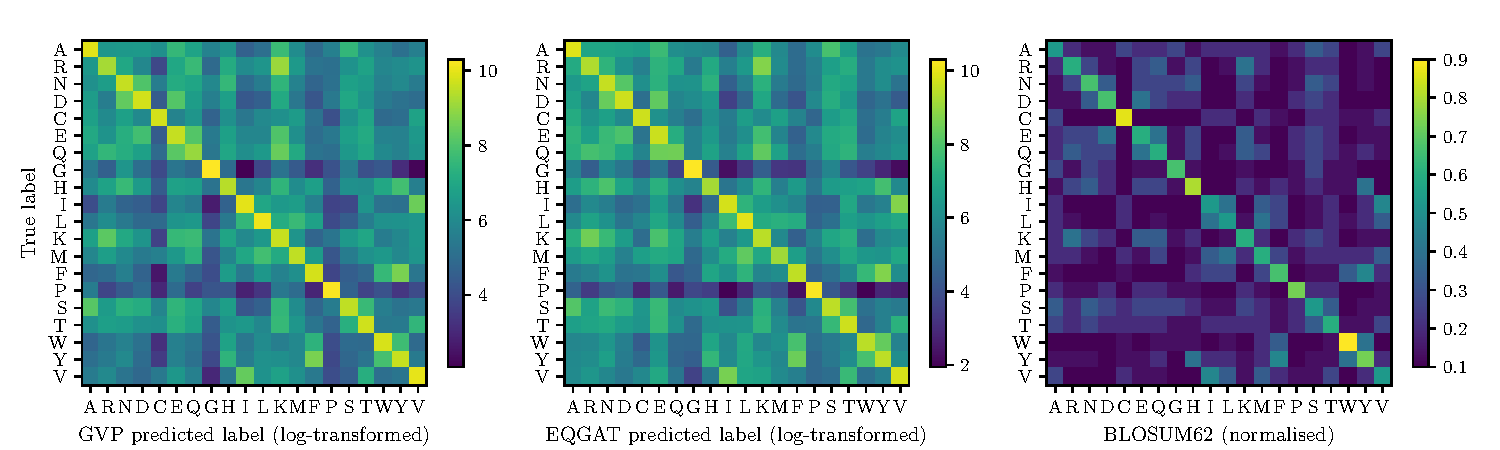
\includegraphics[width=\textwidth]{masters-report/figures/confusion_matrices.pdf}
    \caption{Comparison between the confusion matrices of EQGAT and GVP to the BLOSUM62 matrix.}
    \label{fig:confusions}
\end{figure}


% \subsubsection{Experimental structure vs. AlphaFold structures}


% As mentioned in Section \ref{sec:structure-recovery}, we expect the usage of AlphaFold structures to be detrimental to the overall performance of our models. To check whether this is indeed the case, we perform on ablation study on 14 of the 49 sequences we use in this project. These sequences have both a complete experimental structure and an AlphaFold structure, so we can compare the performance of our models using either one or the other. Since the ablation study presented in Section \ref{mutation-discard} makes it clear that mutations at wrongly predicted positions are detrimental to our models, we perform this second ablation study by also discarding mutations for positions that models get wrong.

% As presented in Tables \ref{ablation-alphafold-global} and \ref{ablation-alphafold-positional}, we find that there isn't a clear relation between using the AlphaFold structure and a decrease in the better than wildtype Spearman correlation, as it seeems to depend on both the model and the ranking strategy used. However, we notice notice that in 3 out of 4 cases, models rank \textit{worse than wildtype} mutations better when using the AlphaFold structure. 

% \begin{table}[!h]
% \caption{Model performance when performing \textbf{global} ranking using either AlphaFold or experimental features. Statistics are averages across 14 sequences.}
% \label{ablation-alphafold-global}
% \vskip 0.15in
% \begin{center}
% \begin{small}
% \begin{sc}
% \begin{tabular}{@{}ccccc@{}}
% \toprule
% \multirow{2}{*}{Model} & \multirow{2}{*}{Structure} & \multicolumn{3}{c}{Spearman's rank correlation}  \\ \cmidrule(l){3-5} 
%                        &                            & Average        & Worse than WT  & Better than WT \\ \midrule
% EQGAT                  & AlphaFold                  & \textbf{0.311} & \textbf{0.177} & 0.136          \\
% EQGAT                  & Experimental               & 0.262          & 0.154          & \textbf{0.157} \\ \midrule
% GVP                    & AlphaFold                  & \textbf{0.237} & \textbf{0.211} & \textbf{0.049} \\
% GVP                    & Experimental               & 0.202          & 0.128          & $-0.011$         \\ \bottomrule
% \end{tabular}
% \end{sc}
% \end{small}
% \end{center}
% \vskip -0.1in
% \end{table}

% \begin{table}[!h]
% \caption{Model performance when performing \textbf{positional} ranking using either AlphaFold or experimental features. Statistics are averages across 14 sequences.}
% \label{ablation-alphafold-positional}
% \vskip 0.15in
% \begin{center}
% \begin{small}
% \begin{sc}

% \begin{tabular}{@{}ccccc@{}}
% \toprule
% \multirow{2}{*}{Model} & \multirow{2}{*}{Structure} & \multicolumn{3}{c}{Spearman's rank correlation}  \\ \cmidrule(l){3-5} 
%                        &                            & Average        & Worse than WT  & Better than WT \\ \midrule
% EQGAT                  & AlphaFold                  & \textbf{0.235} & 0.097          & \textbf{0.149} \\
% EQGAT                  & Experimental               & 0.223          & \textbf{0.128} & 0.118          \\ \midrule
% GVP                    & AlphaFold                  & \textbf{0.253} & \textbf{0.332} & 0.172          \\
% GVP                    & Experimental               & 0.106          & -0.009         & \textbf{0.276} \\ \bottomrule
% \end{tabular}

% \end{sc}
% \end{small}
% \end{center}
% \vskip -0.1in
% \end{table}

% \subsubsection{Full structure vs. local environment}

% One implicit assumption that we make in Section \ref{sec:structure-recovery} is that we input the entire molecule in the GNN, par the masked amino acid position we wish to predict scores for. This may not necessarily be the best approach, because the models are trained on \textit{samples of local environments}, which contain on average 600 nodes, whereas a full molecular structure can have even 4000 nodes. 

% Tables \ref{ablation-local-environment-positional} and \ref{ablation-local-environment-global} show that the EQGAT model benefits from using the entire structure, while the GVP model benefits from using the local environment.
% \begin{table}[!h]
% \caption{Model performance when performing positional ranking using either local environments or the full molecule. Statistics are averaged across 49 sequences.}

% \label{ablation-local-environment-positional}
% % \vskip 0.15in
% \begin{center}
% \begin{footnotesize}
% \begin{sc}
% \begin{tabular}{@{}ccccccc@{}}
% \toprule
% \multirow{2}{*}{Model} & \multirow{2}{*}{Structure} & \multicolumn{3}{c}{Spearman's rank correlation}  & \multirow{2}{*}{\begin{tabular}[c]{@{}c@{}}Top 10 \\ precision\end{tabular}} & \multirow{2}{*}{\begin{tabular}[c]{@{}c@{}}Top 10 \\ recall\end{tabular}} \\ \cmidrule(lr){3-5}
%                        &                            & Average        & Worse than WT  & Better than WT &                                                                              &                                                                           \\ \midrule
% EQGAT                  & Full                       & \textbf{0.223} & \textbf{0.128} & \textbf{0.118} & 0.486                                                                        & \textbf{0.187}                                                            \\
% EQGAT                  & Local                      & 0.203          & 0.039          & 0.041          & \textbf{0.516}                                                               & 0.176                                                                     \\ \midrule
% GVP                    & Full                       & 0.106          & -0.009         & 0.276          & \textbf{0.462}                                                               & \textbf{0.419}                                                            \\
% GVP                    & Local                      & \textbf{0.203} & \textbf{0.104} & \textbf{0.311} & 0.451                                                                        & 0.382                                                                     \\ \bottomrule
% \end{tabular}
% \end{sc}
% \end{footnotesize}
% \end{center}
% \vskip -0.1in
% \end{table}

% \begin{table}[!h]
% \caption{Model performance when performing global ranking using either local environments or the full molecule. Statistics are averaged across 49 sequences.}

% \label{ablation-local-environment-global}
% % \vskip 0.15in
% \begin{center}
% \begin{footnotesize}
% \begin{sc}
% \begin{tabular}{@{}ccccccc@{}}
% \toprule
% \multirow{2}{*}{Model} & \multirow{2}{*}{Structure} & \multicolumn{3}{c}{Spearman's rank correlation}   & \multirow{2}{*}{\begin{tabular}[c]{@{}c@{}}Top 10 \\ precision\end{tabular}} & \multirow{2}{*}{\begin{tabular}[c]{@{}c@{}}Top 10 \\ recall\end{tabular}} \\ \cmidrule(lr){3-5}
%                        &                            & Average        & Worse than WT  & Better than WT  &                                                                              &                                                                           \\ \midrule
% EQGAT                  & Full                       & \textbf{0.262} & \textbf{0.154} & \textbf{0.157}  & 0.491                                                                        & \textbf{0.072}                                                            \\
% EQGAT                  & Local                      & 0.254          & 0.149          & 0.134           & \textbf{0.491}                                                               & 0.047                                                                     \\ \midrule
% GVP                    & Full                       & 0.202          & 0.128          & \textbf{-0.011} & \textbf{0.426}                                                               & 0.100                                                                     \\
% GVP                    & Local                      & \textbf{0.216} & 0.233          & \textbf{-0.031} & 0.392                                                                        & \textbf{0.126}                                                            \\ \bottomrule
% \end{tabular}
% \end{sc}
% \end{footnotesize}
% \end{center}
% \vskip -0.1in
% \end{table}

% \FloatBarrier
\section{Protein fitness prediction}
\label{sec:protein-fitness-prediction}
I evaluate 4 types of ridge regression models: the base model uses only $\mathbf{h}_{\text{one-hot}}$ or $\mathbf{h}_{\text{aa-index}}$ embeddings; while the 3 other types augment the base model with scores from either the EQGAT model, the GVP model, or Tranception, respectively. 

I train each type of ridge regression model, using the two types of embeddings, on each of the 49 DMS assays separately. If we denote the set of single-point mutated sequences in each DMS assay by $S$, then:
\begin{enumerate}
    \item I set aside 20\% of all the sequences in $S$ for testing purposes, and the rest becomes the training set $S_\text{train}$;
    \item I perform cross-validation with the single-point mutated sequences left to determine the best regularisation parameters;
    \item Then, for each $\text{training size}\in\{24, 48, \dots, 216\}$ I sample a subset of $S_{\text{train}}$, train a ridge regression model using the chosen subset, and compute the performance metric $m$;
    \item I repeat the process in Step 3 for 20 times and take the average $m$ for each training size;
    \item I also report the metric $m$ for a ridge regression model that is trained on the full $S_{\text{train}}$. 
\end{enumerate}

Figure \ref{one-hot-regression} summarises the performance of the ridge regression models. In the case of fitness prediction for better than wildtype mutations, my results are similar to the results reported by \citet{chloe-hsu}: the augmented linear models allow us to surpass the baseline zero-shot fitness prediction models with as few as 100 datapoints in the case of the model augmented with EQGAT scores. While the linear model augmented with Tranception scores performs best overall, I point out that Tranception is fine-tuned to predict protein fitness, while the scores retrieved from the structure-based models merely represent the confidence in a certain amino acid for a target position.

\begin{figure}[!htb]
    \centering
    \subfigure[\raggedright 
    The EQGAT-augmented model is the only model that exceeds the Tranception baseline for 216 training samples.]{ 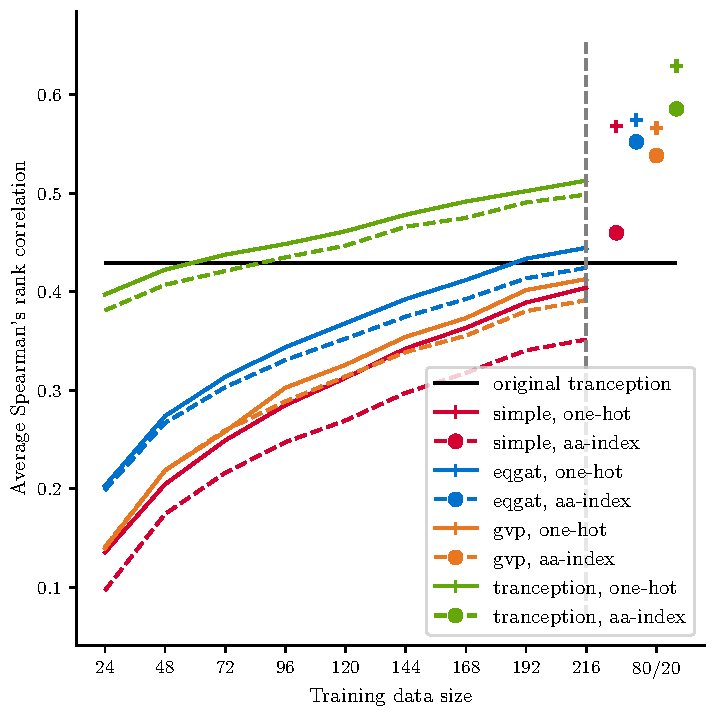
\includegraphics[width=0.45\textwidth]{masters-report/figures/spearmanr_all_square.pdf}\label{average-spearman-ridge-plot}} 
    \hspace{0.1in}
    \subfigure[We can improve the better than wildtype fitness prediction performance above the Tranception baseline (in black) across all regression models by training on as few as 144 data points.]{ 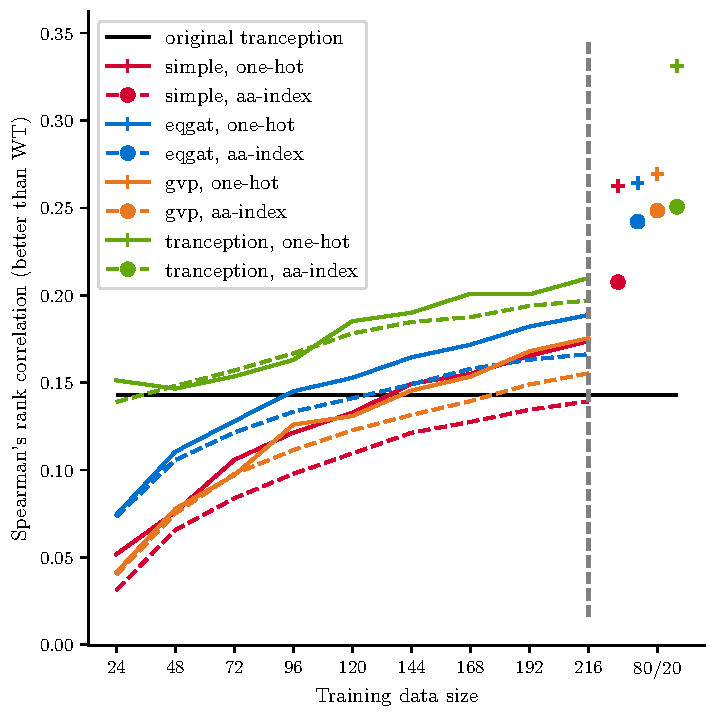
\includegraphics[width=0.45\textwidth]{masters-report/figures/better_than_WT_spearmanr_all_square.pdf}}
    \caption{Performance on mutations for four regression models using two types of embeddings. Statistics are aggregated across 49 DMS assays.}
    \label{one-hot-regression}
\end{figure}

I note from Figure \ref{average-spearman-ridge-plot} that with the exception of the EQGAT model, none of the other models exceed the unsupervised Tranception baseline within 216 training data points when I consider the Spearman rank correlation for the prediction of \textbf{all} fitness variants.

The augmented regressions with structure-based model scores can outperform the Tranception baseline on the better than wildtype Spearman correlation, but fail to do so within 216 samples for the overall Spearman correlation. This can be explained through the fact that, as we see in Table \ref{generation-results}, Tranception is far better than structure-based models at predicting the fitness of bad mutations. Hence, the baseline for overall fitness prediction is stronger. 






\chapter{Conclusions}

This project has investigated the power of pre-trained structure-based models for the generation of viable protein mutations. I trained two EGNN models, namely the GVP \cite{gvp2} and the EQGAT \cite{eqgat2} on the task of residue identity prediction, achieving state-of-the-art performance with the GVP model on predicting better than wildtype mutations. 

I compared the performance of these models to sequence-based approaches across 49 DMS assays, and concluded that they achieve competitive performance to state-of-the-art methods when ranking mutations that are better than the wildtype protein, while also being trained of \textbf{15,909x} fewer molecules. 

Additionally, I show how the positional scores generated by these methods can be successfully used in a low-data regime by augmenting ridge-regression models in order to predict protein fitness across 49 DMS assays.

\section{Future work}
While the results of this project look promising, the analysis is still limited in scope. I identify a couple of areas that future work should focus on.

\paragraph{Hetero-oligomeric assemblies.} This project does not analyse the performance of structure-based models on hetero-oligomeric assemblies, due to the engineering complexity required to perform mutations across non-identical protein chains. Future work should expand on the results of this project to devise good ranking strategies for these complex macromolecules. 

\paragraph{Multiple-point mutations.} My project focuses on single-point mutations, yet many successfully engineered proteins may require multiple amino acid mutations across separate sites. Future work on multiple-point mutations should focus on investigating epistasis in molecular chains: how likely are \textit{pairs} or \textit{triples} of amino acids to fold together in certain conformations, and how can can we take advantage of this via structure-based models?

\paragraph{Different kinds of fitness.} The ProteinGym dataset \cite{tranception} contains a wide range of mutational data across 87 different proteins. Some of these proteins are viruses (e.g., SARS-CoV-2), some are bacteria (Baker's yeast), while others are proteins found in humans. While mutations across all DMS assays receive a numerical fitness score, this fitness has different meanings, depending on the context: some types of fitness relate to thermostability (e.g., the fitness optimised by \citet{Lu2022} when engineering plastic proteins), while others relate to infectivity, in the case of viruses. I expect structure-based methods to be better at predicting thermostability, so future work should focus on identifying the precise types of fitness structure-based methods excel at. 

\paragraph{Dataset improvements.} The pre-trained models used in this project were trained on the ATOM3D RES dataset \cite{atom-3d}, which is open source, with the best model achieving an accuracy of \textbf{58\%}. The approach that uses 3D-CNNs, namely MutCompute \cite{mutcompute}, achieves an accuracy of around 70\% on a proprietary dataset. The authors describe data engineering strategies they employed to transform the dataset in such a way that would help the trained models to better generalise to unseen proteins and understand the fitness landscape of the structure. Hence, the ATOM3D RES dataset itself  may be a bottleneck in the development of more powerful structure-based models, and I encourage future work to focus on improving this dataset. 

\paragraph{Ranking strategies.} The ranking strategies used in this project are straightforward, focusing either on position confidence or on overall amino acid confidence. However, not all amino acids are equally likely to appear in proteins, with certain groups of amino acids being more easily substituted with one another, as we saw from the BLOSUM62 matrix. Ranking strategies that take these behaviours into consideration could compare the KL divergence of subsets of related amino acids to determine where the model identified interesting candidates.

Ultimately, this project has investigated the usage of EGNNs for protein engineering. Throughout this research, significant strides have been made in understanding the potential of EGNNs in enhancing protein design and optimisation, with results indicating the efficacy and potential of structure-based models in addressing key challenges in computational protein engineering.

I emphasise that this research field is still in its infancy. While EGNNs have shown promising results, there is much work to be done to fully explore their capabilities and address the existing limitations. I believe the potential of these models in protein engineering is vast, and future research efforts should aim to build upon the foundation laid by this project.

\label{lastcontentpage} % end page count here
%TC:ignore
\bibliographystyle{unsrtnat}
\bibliography{reference}
% For bibLaTeX users:
% \printbibliography

\clearpage


\appendix
\chapter{Appendix}
\section{Correlation to Tranception ranking}
\label{tranception-correlation}

\begin{table}[!h]
\centering
\caption{Average Spearman rank correlation (for better than wildtype predictions) between Tranception and structure-based models. }
\vskip 0.15in
\begin{tabular}{@{}ccc@{}}
\toprule
Model                  & Ranking    & Correlation to Tranception \\ \midrule
\multirow{2}{*}{EQGAT} & Global     & 0.212                      \\
                       & Positional & 0.146                      \\ \midrule
\multirow{2}{*}{GVP}   & Global     & 0.147                      \\
                       & Positional & 0.073                      \\ \bottomrule
\end{tabular}

\end{table}

\begin{figure}[!h]
    \centering
    \subfigure[\raggedright Spearman's rank correlation between the ranking made by the GVP model and Tranception.]{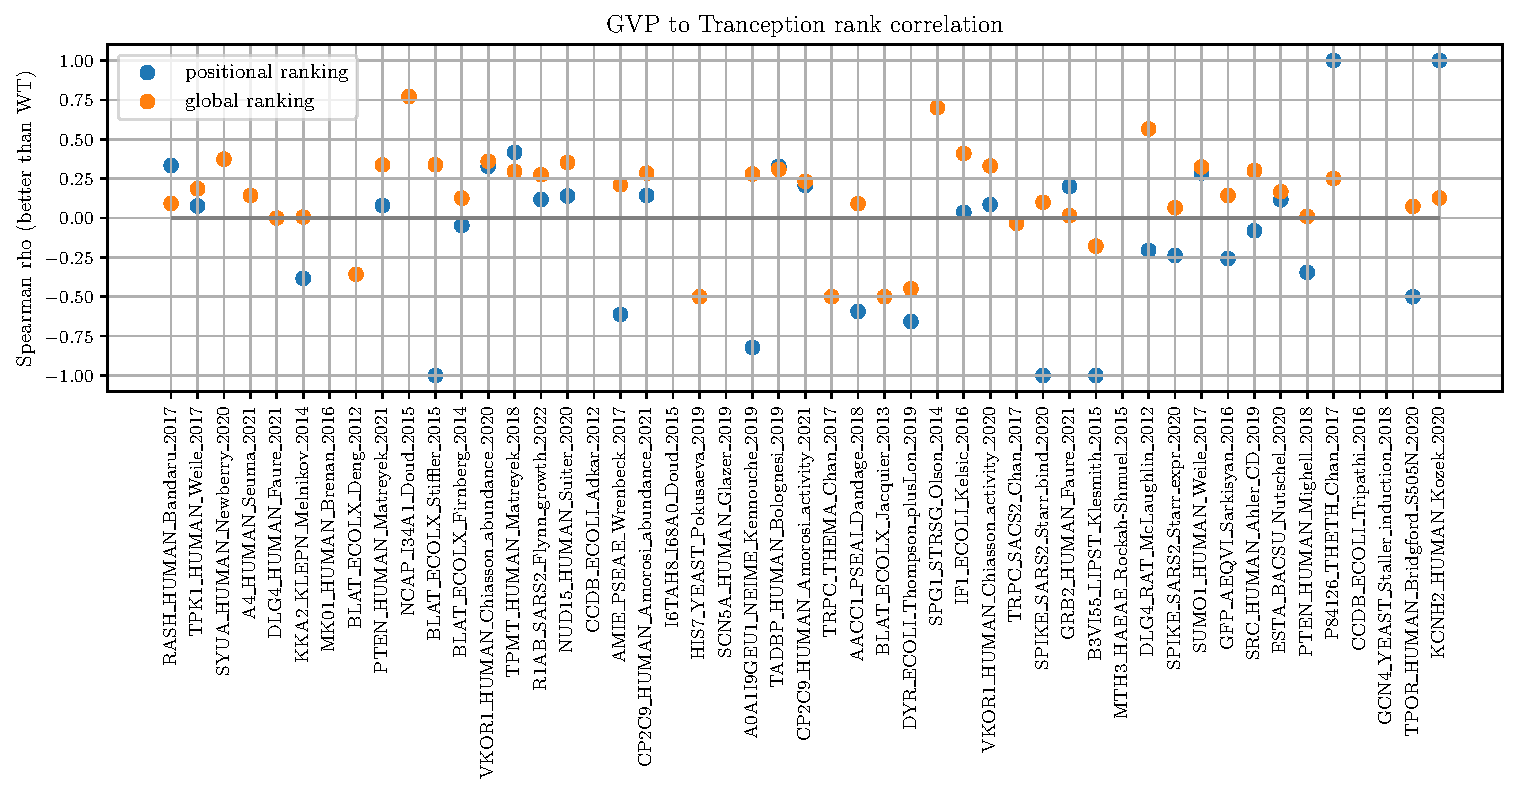
\includegraphics[width=\textwidth]{masters-report/figures/GVP_tranception_corr.pdf}}
    % \label{fig:gvp-tranception-corr}
    \vspace{1cm}
    \subfigure[\raggedright Spearman's rank correlation between the ranking made by the EQGAT model and Tranception.]{
    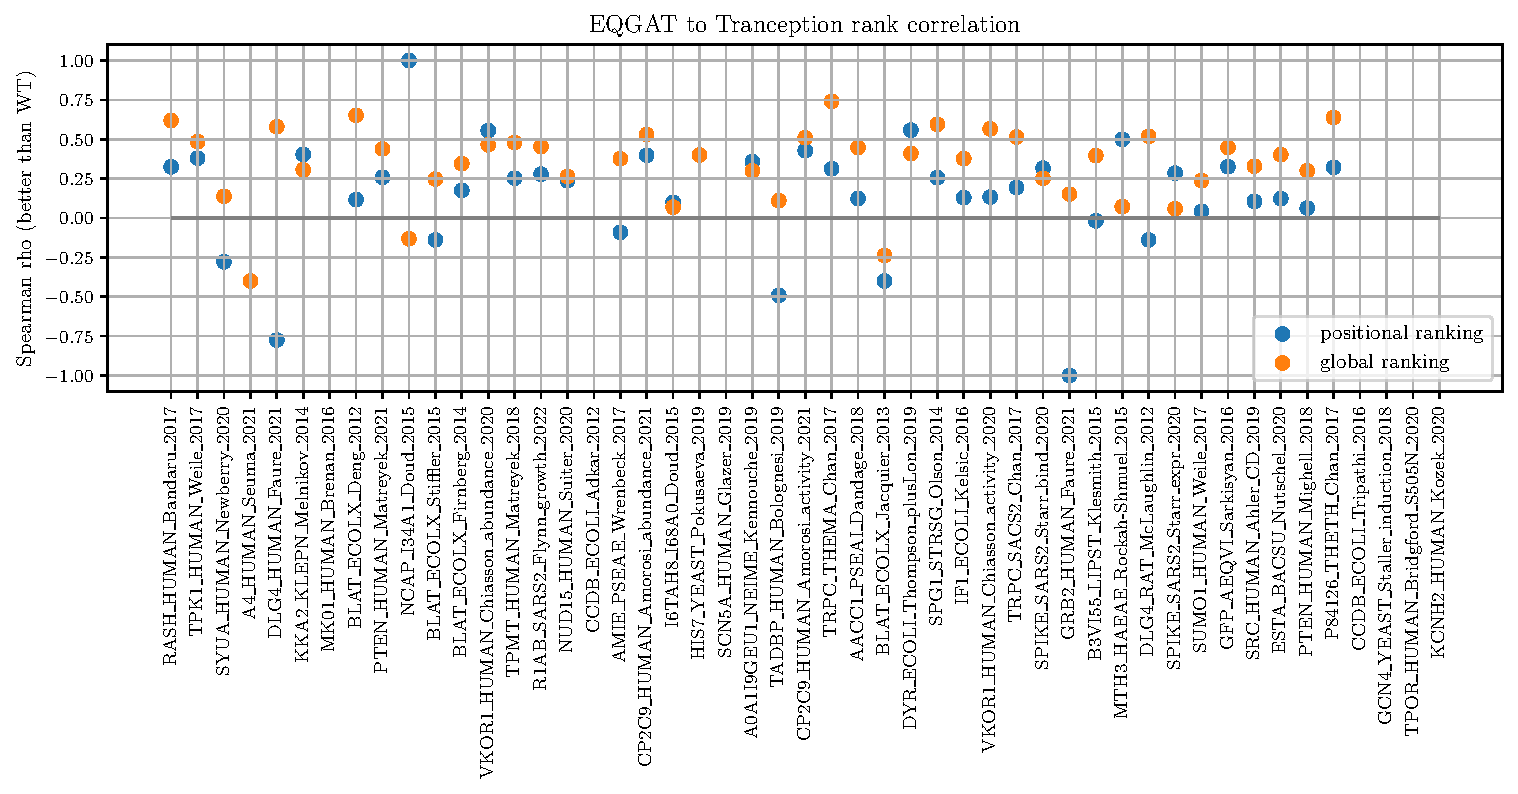
\includegraphics[width=\textwidth]{masters-report/figures/EQGAT_tranception_corr.pdf}}
    % \label{fig:eqgat-tranception-corr}
\caption{Correlation between rankings made by Tranception and rankings made by our structure-based models. Missing values indicate that \textbf{fewer than 2} mutations that are better than the wildtype were proposed.}
\end{figure}
\label{lastpage}

\FloatBarrier
\clearpage
\section{Other ablation studies}
\subsection{Experimental structure vs. AlphaFold structures}
\label{appendix-exp-vs-alphafold}
As mentioned in Section \ref{sec:structure-recovery}, we expect the usage of AlphaFold structures to be detrimental to the overall performance of our models. To check whether this is indeed the case, we perform on ablation study on 14 of the 49 sequences we use in this project. These sequences have both a complete experimental structure and an AlphaFold structure, so we can compare the performance of our models using either one or the other. Since the ablation study presented in Section \ref{mutation-discard} makes it clear that mutations at wrongly predicted positions are detrimental to our models, we perform this second ablation study by also discarding mutations for positions that models get wrong.

As presented in Tables \ref{ablation-alphafold-global} and \ref{ablation-alphafold-positional}, we find that there isn't a clear relation between using the AlphaFold structure and a decrease in the better than wildtype Spearman correlation, as it seeems to depend on both the model and the ranking strategy used. However, we notice notice that in 3 out of 4 cases, models rank \textit{worse than wildtype} mutations better when using the AlphaFold structure. 

\begin{table}[!h]
\caption{Model performance when performing \textbf{global} ranking using either AlphaFold or experimental features. Statistics are averages across 14 sequences.}
\label{ablation-alphafold-global}
\vskip 0.15in
\begin{center}
\begin{small}
\begin{sc}
\begin{tabular}{@{}ccccc@{}}
\toprule
\multirow{2}{*}{Model} & \multirow{2}{*}{Structure} & \multicolumn{3}{c}{Spearman's rank correlation}  \\ \cmidrule(l){3-5} 
                       &                            & Average        & Worse than WT  & Better than WT \\ \midrule
EQGAT                  & AlphaFold                  & \textbf{0.311} & \textbf{0.177} & 0.136          \\
EQGAT                  & Experimental               & 0.262          & 0.154          & \textbf{0.157} \\ \midrule
GVP                    & AlphaFold                  & \textbf{0.237} & \textbf{0.211} & \textbf{0.049} \\
GVP                    & Experimental               & 0.202          & 0.128          & $-0.011$         \\ \bottomrule
\end{tabular}
\end{sc}
\end{small}
\end{center}
\vskip -0.1in
\end{table}

\begin{table}[!h]
\caption{Model performance when performing \textbf{positional} ranking using either AlphaFold or experimental features. Statistics are averages across 14 sequences.}
\label{ablation-alphafold-positional}
\vskip 0.15in
\begin{center}
\begin{small}
\begin{sc}

\begin{tabular}{@{}ccccc@{}}
\toprule
\multirow{2}{*}{Model} & \multirow{2}{*}{Structure} & \multicolumn{3}{c}{Spearman's rank correlation}  \\ \cmidrule(l){3-5} 
                       &                            & Average        & Worse than WT  & Better than WT \\ \midrule
EQGAT                  & AlphaFold                  & \textbf{0.235} & 0.097          & \textbf{0.149} \\
EQGAT                  & Experimental               & 0.223          & \textbf{0.128} & 0.118          \\ \midrule
GVP                    & AlphaFold                  & \textbf{0.253} & \textbf{0.332} & 0.172          \\
GVP                    & Experimental               & 0.106          & -0.009         & \textbf{0.276} \\ \bottomrule
\end{tabular}

\end{sc}
\end{small}
\end{center}
\vskip -0.1in
\end{table}

\subsection{Full structure vs. local environment}
\label{appendix-full-vs-local}
One implicit assumption that we make in Section \ref{sec:structure-recovery} is that we input the entire molecule in the GNN, par the masked amino-acid position we wish to predict scores for. This may not necessarily be the best approach, because the models are trained on \textit{samples of local environments}, which contain on average 600 nodes, whereas a full molecular structure can have even 4000 nodes. 

Tables \ref{ablation-local-environment-positional} and \ref{ablation-local-environment-global} show that the EQGAT model benefits from using the entire structure, while the GVP model benefits from using the local environment.
\begin{table}[!h]
\caption{Model performance when performing positional ranking using either local environments or the full molecule. Statistics are averaged across 49 sequences.}

\label{ablation-local-environment-positional}
% \vskip 0.15in
\begin{center}
\begin{footnotesize}
\begin{sc}
\begin{tabular}{@{}ccccccc@{}}
\toprule
\multirow{2}{*}{Model} & \multirow{2}{*}{Structure} & \multicolumn{3}{c}{Spearman's rank correlation}  & \multirow{2}{*}{\begin{tabular}[c]{@{}c@{}}Top 10 \\ precision\end{tabular}} & \multirow{2}{*}{\begin{tabular}[c]{@{}c@{}}Top 10 \\ recall\end{tabular}} \\ \cmidrule(lr){3-5}
                       &                            & Average        & Worse than WT  & Better than WT &                                                                              &                                                                           \\ \midrule
EQGAT                  & Full                       & \textbf{0.223} & \textbf{0.128} & \textbf{0.118} & 0.486                                                                        & \textbf{0.187}                                                            \\
EQGAT                  & Local                      & 0.203          & 0.039          & 0.041          & \textbf{0.516}                                                               & 0.176                                                                     \\ \midrule
GVP                    & Full                       & 0.106          & -0.009         & 0.276          & \textbf{0.462}                                                               & \textbf{0.419}                                                            \\
GVP                    & Local                      & \textbf{0.203} & \textbf{0.104} & \textbf{0.311} & 0.451                                                                        & 0.382                                                                     \\ \bottomrule
\end{tabular}
\end{sc}
\end{footnotesize}
\end{center}
\vskip -0.1in
\end{table}

\begin{table}[!h]
\caption{Model performance when performing global ranking using either local environments or the full molecule. Statistics are averaged across 49 sequences.}

\label{ablation-local-environment-global}
% \vskip 0.15in
\begin{center}
\begin{footnotesize}
\begin{sc}
\begin{tabular}{@{}ccccccc@{}}
\toprule
\multirow{2}{*}{Model} & \multirow{2}{*}{Structure} & \multicolumn{3}{c}{Spearman's rank correlation}   & \multirow{2}{*}{\begin{tabular}[c]{@{}c@{}}Top 10 \\ precision\end{tabular}} & \multirow{2}{*}{\begin{tabular}[c]{@{}c@{}}Top 10 \\ recall\end{tabular}} \\ \cmidrule(lr){3-5}
                       &                            & Average        & Worse than WT  & Better than WT  &                                                                              &                                                                           \\ \midrule
EQGAT                  & Full                       & \textbf{0.262} & \textbf{0.154} & \textbf{0.157}  & 0.491                                                                        & \textbf{0.072}                                                            \\
EQGAT                  & Local                      & 0.254          & 0.149          & 0.134           & \textbf{0.491}                                                               & 0.047                                                                     \\ \midrule
GVP                    & Full                       & 0.202          & 0.128          & \textbf{-0.011} & \textbf{0.426}                                                               & 0.100                                                                     \\
GVP                    & Local                      & \textbf{0.216} & 0.233          & \textbf{-0.031} & 0.392                                                                        & \textbf{0.126}                                                            \\ \bottomrule
\end{tabular}
\end{sc}
\end{footnotesize}
\end{center}
\vskip -0.1in
\end{table}

\clearpage


\section{Per-dataset performance breakdown}
\label{appendix:per-dataset-breakdown}
\begin{figure}[!h]
    \centering
    \subfigure[Per-dataset performance of EQGAT.]{
        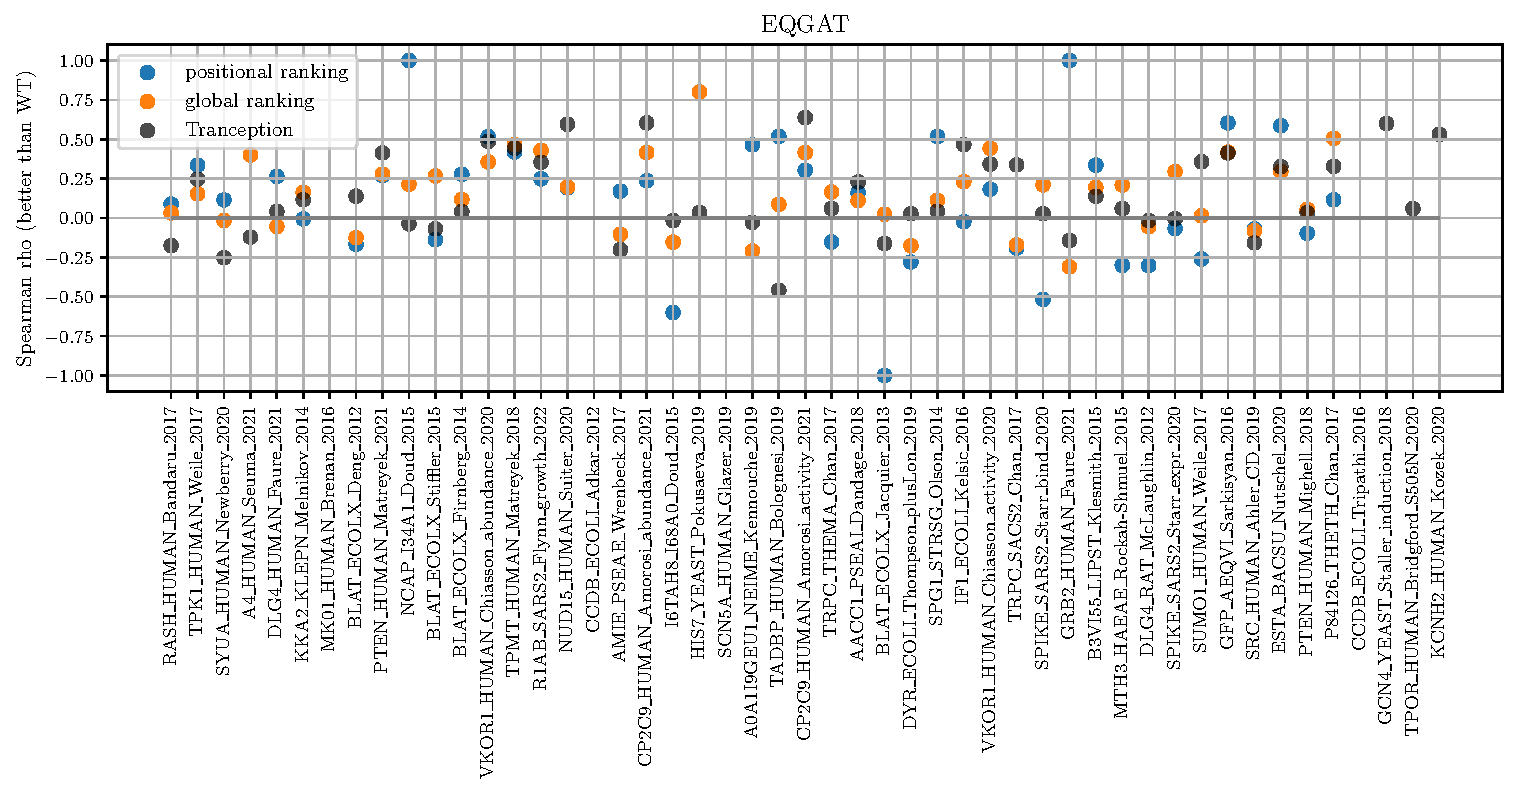
\includegraphics[width=\textwidth]{masters-report/figures/EQGAT_better_than_WT_per_dataset.pdf}
    }
    \vspace{1cm}
    \subfigure[Per-dataset performance of GVP.]{
        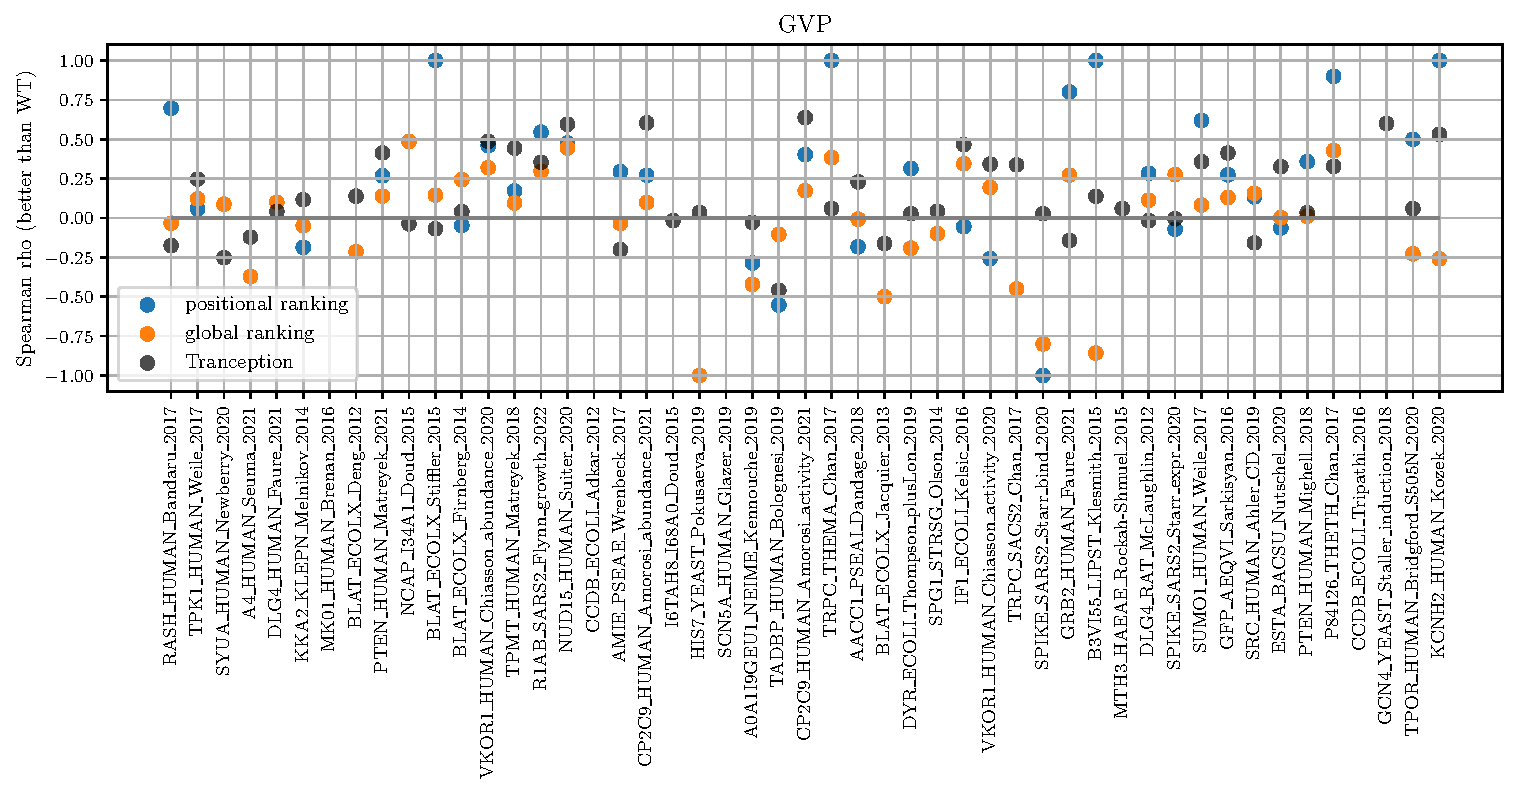
\includegraphics[width=\textwidth]{masters-report/figures/GVP_better_than_WT_per_dataset.pdf}
    }
    \caption{Breakdown of the better than wildtype Spearman rank correlation on our structure-based models, with Tranception as reference. Missing values indicate that \textbf{at most} 1 mutations proposed were better than the wildtype.}
    \label{per-dataset-breakdown}
\end{figure}
\clearpage
\section{Training and mutation generation commands}
Terminal command used to train the GVP model:

\begin{quote}
\begin{verbatim}
python3 ~/rds/hpc-work/partIII-amino-acid-prediction/res_task/main.py
--model gvp 
--data_file ~/rds/hpc-work/split-by-cath-topology/data/ 
--slurm --gpus 1 --num_nodes 1  
--batch_size 64 --n_layers 5 
--data_workers 16 --epochs 40 
\end{verbatim}
\end{quote}
Terminal command used to train the EQGAT model:
\begin{quote}
\begin{verbatim}
python3 ~/rds/hpc-work/partIII-amino-acid-prediction/res_task/main.py 
--model eqgat 
--data_file ~/rds/hpc-work/split-by-cath-topology/data/ 
--slurm --gpus 1 --num_nodes 1  
--batch_size 64 --n_layers 5 
--data_workers 16 --epochs 40 
\end{verbatim}
\end{quote}
Terminal command used to generate mutations with the GVP model (discarding mutations at wrongly predicted positions and using experimental structures when available):
\begin{quote}
\begin{verbatim}
python3 mutations_eval.py --mapper './data/mapping.csv' 
--model_path '~/part3-res-prediction-diss/lf9niuld/checkpoints/
        epoch=40-step=2230113.ckpt' 
--batch_size 2 --model 'gvp' 
--correct_only --out_dir './data'
\end{verbatim}
\end{quote}
Terminal command used to generate mutations with the EQGAT model (discarding mutations at wrongly predicted positions and using experimental structures when available):
\begin{quote}
\begin{verbatim}
python3 mutations_eval.py --mapper './data/mapping.csv' 
--model_path '~/part3-res-prediction-diss/nvqpopw8/checkpoints/
        epoch=39-step=2175720.ckpt'
--batch_size 2 --correct_only 
--model 'eqgat' --out_dir './data'
\end{verbatim}
\end{quote}
\end{document}
